% ===================================================================
%  Beamer: IAEA PT 多维度分析 (2021-2025)
% ===================================================================
\documentclass[10pt,aspectratio=169]{beamer}

\usepackage[UTF8]{ctex}
\setCJKmainfont{SimSun}[BoldFont=SimHei]
\setCJKsansfont{Microsoft YaHei}
\setCJKmonofont{KaiTi}
\usepackage{graphicx,booktabs,tikz,xcolor,amsmath}

\definecolor{mainblue}{RGB}{0,76,153}
\definecolor{accent}{RGB}{204,51,51}
\definecolor{darkgray}{RGB}{51,51,51}
\definecolor{lightgray}{RGB}{242,242,242}
\definecolor{midblue}{RGB}{0,122,204}

\usetheme{default}
\setbeamertemplate{navigation symbols}{}

\setbeamertemplate{frametitle}{%
  \vspace{0.2cm}
  {\large\color{mainblue}\bfseries\insertframetitle}\par
  \vspace{0.05cm}
  \textcolor{mainblue}{\rule{\textwidth}{1pt}}
  \vspace{-0.2cm}
}
\setbeamercolor{title}{fg=mainblue}
\setbeamercolor{frametitle}{fg=mainblue}
\setbeamercolor{normal text}{fg=darkgray}
\setbeamercolor{itemize item}{fg=midblue}
\setbeamercolor{enumerate item}{fg=mainblue}
\setbeamercolor{block title}{fg=white,bg=mainblue}
\setbeamercolor{block body}{fg=darkgray,bg=lightgray}

\usebackgroundtemplate{%
  \begin{tikzpicture}[remember picture,overlay]
    \node[anchor=south west,inner sep=0pt] at (current page.south west)
      {
\includegraphics[height=0.5cm]{template_img_png_0.png}};
    \node[anchor=north east,inner sep=0pt,xshift=-0.2cm,yshift=-0.1cm] at (current page.north east)
      {
\includegraphics[height=1.1cm]{template_img_png_5.png}};
    \node[anchor=north east,inner sep=0pt,xshift=-1.5cm] at (current page.north east)
      {
\includegraphics[height=1.4cm]{template_img_png_1.png}};
  \end{tikzpicture}
}

% Compact itemize
\newenvironment{tightitemize}{\begin{itemize}\setlength{\itemsep}{2pt}\setlength{\parskip}{0pt}\setlength{\parsep}{0pt}}{\end{itemize}}
\newenvironment{tightenumerate}{\begin{enumerate}\setlength{\itemsep}{2pt}\setlength{\parskip}{0pt}\setlength{\parsep}{0pt}}{\end{enumerate}}

\title{IAEA能力验证中辐射监测实验室的长期性能评估}
\subtitle{——以本实验室为例（2021—2025年）}
\author{李云龙}
\institute{生态环境部辐射环境监测技术中心 \\ 生态环境部辐射环境监测重点实验室}
\date{2026年6月}

\begin{document}

% ===== SLIDE 1: Title =====
{
\setbeamertemplate{background}{
  \begin{tikzpicture}[remember picture,overlay]
    \fill[mainblue] (current page.south west) rectangle (current page.north east);
  \end{tikzpicture}
}
\begin{frame}
  \color{white}
  \centering\vspace{1.2cm}
  {\Huge\bfseries IAEA能力验证中辐射监测实验室的长期性能评估}\\[0.6cm]
  {\Large ——以本实验室为例（2021—2025年）}\\[1.2cm]
  {\large 李云龙}\\[0.2cm]
  {\small 生态环境部辐射环境监测技术中心 \\ 生态环境部辐射环境监测重点实验室}\\[0.4cm]
  {\small 2026年6月}
\end{frame}
}

% ===== SLIDE 2: IAEA PT 项目介绍 =====
\begin{frame}{IAEA 能力验证项目概况}
  \small      
	\centering
      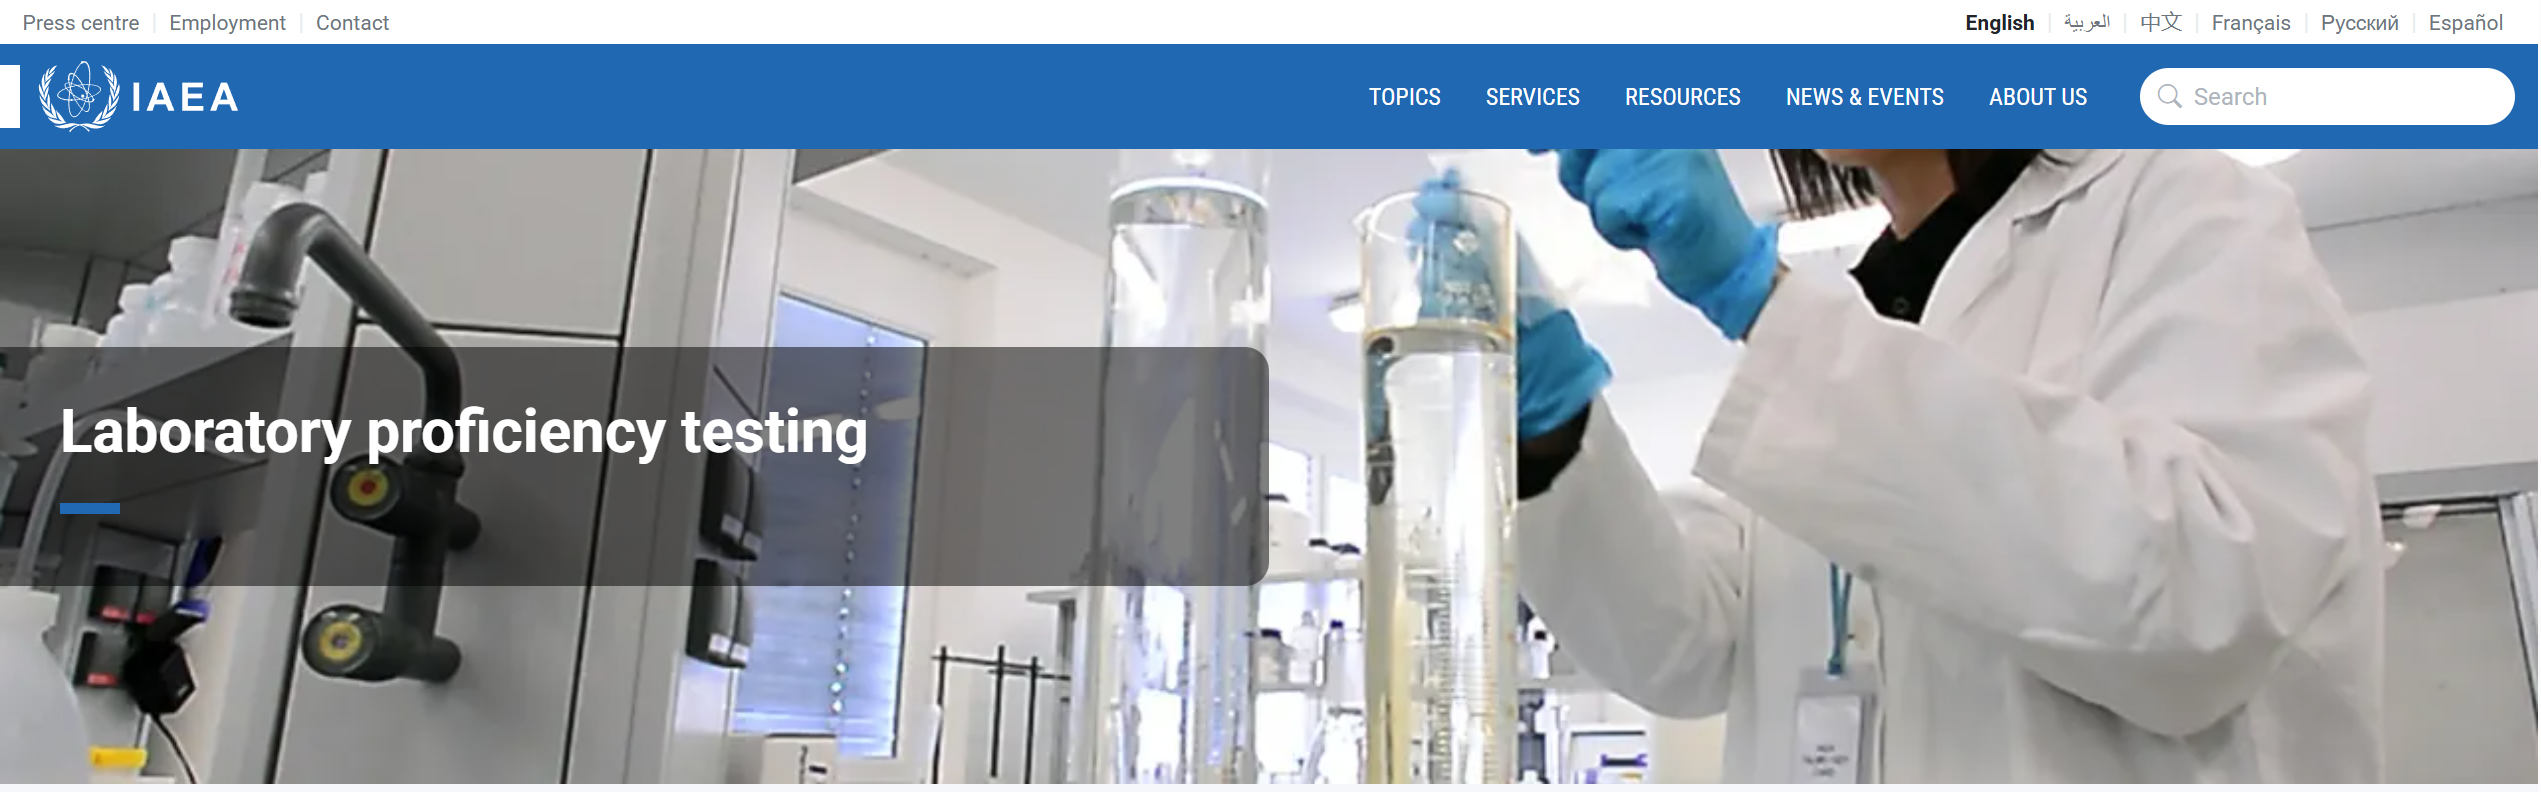
\includegraphics[width=0.8\textwidth,keepaspectratio]{IAEA_PT.png}
      \begin{block}{\small 项目背景与目的}
        IAEA 陆地环境放射化学实验室（TERC）自20世纪70年代起，每年组织全球能力验证（PT）和实验室间比对（ILC），面向成员国及 ALMERA（环境放射性测量能力验证实验室网络）实验室，旨在：
        \begin{tightitemize}
	\scriptsize
          \item 监测和评估参与实验室的放射性核素分析能力
          \item 识别技术差距与待改进领域，推动方法发展
          \item 促进全球环境放射性测量数据的可比性与互认
        \end{tightitemize}
      \end{block}
\end{frame}

\begin{frame}{IAEA 能力验证项目概况}
      \begin{block}{\small 近年 PT 轮次 (2021--2026)}
        \centering\scriptsize
        \begin{tabular}{@{}ccccc@{}}
          \toprule
          \textbf{年份} & \textbf{PT 编号} & \textbf{样品基质} & \textbf{参加实验室个数}  & \textbf{分析项目个数}\\
          \midrule
          2021 & TEL-2021-03  & 水样3、植物样1（日本竹子）、表面擦拭样1 &  270 & 28\\
          2022 & TERC-2022-01 & 水样3、土壤$\gamma$谱文件、表面擦拭样1 &  277 & 56\\
          2023 & TERC-2023-01 & 水样2、土壤样1（日本土壤）、表面擦拭样3 &  319 & 40\\
          2024 & TERC-2024-01 & 水样1、沉积物1、铝土矿1、表面擦拭样1 &  472 &47\\
          2025 & TERC-2025-01 & 水样2、土壤样1、植物样1、表面擦拭样1 & 399 & 42\\
          2026 & TERC-2026-01 & 水样2、土壤样1、表面擦拭样1 &  & \\
          \bottomrule
        \end{tabular}
      \end{block}
  \begin{columns}
    \begin{column}{0.5\textwidth}    
	  \begin{block}{\small 测试内容与形式}
        \begin{tightitemize}
	\scriptsize
          \item 发放加标环境样品，测定\textcolor{accent}{人工与天然来源}的 $\alpha$、$\beta$、$\gamma$ 放射性核素
          \item 参试实验室可自由选择报告核素（非强制全测），截止日后数月内获独立评价报告
        \end{tightitemize}
      \end{block}
	\scriptsize
 2026 IAEA PT链接：\href{https://analytical-reference-materials.iaea.org/iaea-terc-2026-01}{https://analytical-reference-materials.iaea.org/iaea-terc-2026-01}
    \end{column}
    \begin{column}{0.5\textwidth}
      \centering
      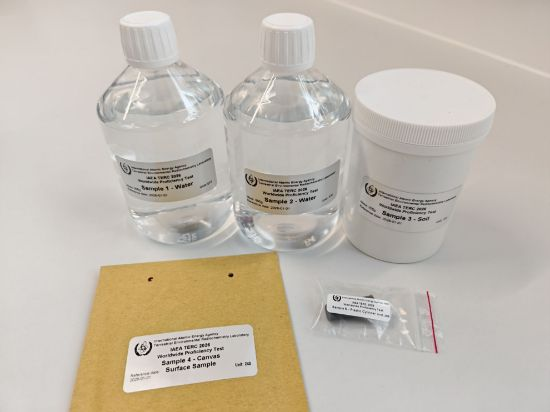
\includegraphics[width=0.7\textwidth,keepaspectratio]{samples.jpeg}
    \end{column}
  \end{columns}

\end{frame}

% ===== SLIDE 3: 背景 =====
\begin{frame}{IAEA 能力验证评估方法 (ISO 13528)}
  \small
  \begin{block}{\small  对于给定真值(Target value)的项目}
    \textbf{正确度 (Trueness):\;}
    相对偏差$\text{RB} = \frac{x_{\text{rep}} - x_{\text{ref}}}{x_{\text{ref}}} \times 100\%$，若 $|\text{RB}| \leq \text{最大可接受偏差(MARB)}$ 则评为"A"\\[1pt]
    \textbf{精密度 (Precision):\;}
    $P = \sqrt{(\frac{u_{\text{ref}}}{x_{\text{ref}}})^2 + (\frac{u_{\text{rep}}}{x_{\text{rep}}})^2} \times 100\%$，需同时满足:\; $|\text{RB}| \leq k \cdot P$ ($k{=}2.58$) $\wedge$ $P \leq \text{MARB}$\\[1pt]
    \textbf{最终评分:\;}
    \textcolor{mainblue}{accepted(A)} = 正确度A $\wedge$ 精密度A \;
    \textcolor{accent}{warning(W)} = 正确度A $\wedge$ 精密度N \;
    \textbf{not accepted(N)} = 正确度N
  \end{block}
  \begin{block}{\small 对于未给定真值的项目(intercomparison)}
    \textbf{Z-Score:\;}
    $Z = \frac{x_{\text{rep}} - x_{\text{ref}}}{\sigma_{\text{PT}}}$，$x_{\text{ref}}$和$\sigma_{\text{PT}}$为所有报告结果的稳健平均值和稳健标准差\\
    $|Z|{\leq}2 {\to}$ A, $2{<}|Z|{<}3 {\to}$ W, $|Z|{\geq}3 {\to}$ N
  \end{block}
  \begin{block}{问题提出}
    传统A/W/N报告仅提供简单的结果参考；长期得"A"的实验室仍可能存在系统偏差；项目难度因核素、基质和年份而异——需要\textcolor{accent}{综合考量准确度、一致性和同行相对表现的多维度评估框架}。
  \end{block}
\end{frame}

% ===== SLIDE 3: 单位简介 =====
\begin{frame}{单位简介：生态环境部辐射环境监测技术中心}
  \small
    \begin{tightitemize}
      \item 始建于1984年，为浙江省省生态环境厅直属事业单位
	\item 拥有生态环境部辐射环境监测重点实验室
      \item \textbf{全国辐射环境监测的技术中心、龙头单位}，承担全国辐射环境监测技术支撑
      \item 2024年成为IAEA认定的\textcolor{accent}{环境放射性测量能力验证实验室网络(ALMERA)}成员
    \end{tightitemize}
  \begin{block}{\small 核心职能}
    \begin{columns}
      \begin{column}{0.50\textwidth}
        \begin{tightitemize}
	\scriptsize
          \item 全国辐射环境监测技术标准制定
          \item 全国辐射环境质量监测与评价
          \item 国家辐射环境监测网络运行管理
          \item 核与辐射事故应急监测技术支撑
        \end{tightitemize}
      \end{column}
      \begin{column}{0.50\textwidth}
	\scriptsize
        \begin{tightitemize}
          \item 放射性废物(源)安全管理
          \item 辐射环境自动监测站建设与运行
          \item 国际交流与能力验证
          \item 全国辐射监测技术培训与指导
        \end{tightitemize}
      \end{column}
    \end{columns}
  \end{block}
  \begin{block}{\small 人才队伍}
全站共有137人，其中专业技术干部人员121人（硕士及以上88人）。国家生态环境保护专家委员会委员1名、生态环境部核安全专家委员会委员1名，12人入选生态环境部“三五”人才。
  \end{block}
\end{frame}

% ===== SLIDE 4: 五个维度 =====
\begin{frame}{方法论：五个互补分析维度}
将所有分析项目划分为"核素+方法+基质"组合，如用$\gamma$能谱法测水中${}^{137}\text{Cs}$活度浓度标记为"Cs137 Gamma Water"。从以下五个维度分析结果：
  \small
\begin{itemize}
	\item \textbf{项目难度系数和通过率}：对每个分析项目计算其难度系数和通过率，四层分类: Very Easy / Easy / Moderate / Hard
	\item \textbf{难度时间趋势}：跨年匹配同一核素-方法-基质项目，加权平均合并变体，追踪难度变化
	\item \textbf{实验室比对排名}：参与广度/A计数排名 + 项目内百分位排序
	\item \textbf{难度分层分析}：按四级难度分层，评估通过率 vs. 全球均值
	\item \textbf{项目内相对偏差排名}：偏差分布图 + 百分位排名 + 跨年度热力图
\end{itemize}
本单位：12$\to$35项/年 (累计135次测量，133核素-方法-基质项目)。匿名编号：211/8/43/5/15。
\end{frame}

% ===== SLIDE 7a: Bullet 1 —— 水中人工核素 (bars 1-5, top) =====
\begin{frame}{维度1：项目难度系数与通过率}
  \begin{columns}
    \begin{column}{0.43\textwidth}
      \small
      \begin{block}{\small 难度系数和通过率}
        \textbf{难度系数} $D_{j,y} = 1 - N^{(A)}_{j,y} / N^{\text{(all labs)}}_y$\\[1pt]
        \textbf{通过率} $P_{j,y} = N^{(A)}_{j,y} / N^{\text{(in project)}}_j$
      \end{block}
      \begin{tightitemize}
        \item \textcolor{red}{水中人工放射性核素}难度\textbf{最低}、通过率最高
        \item Co-60, Cs-137, Cs-134, Ba-133, Na-22
        \item  活度较高，$\gamma$能谱法成熟
      \end{tightitemize}
    \end{column}
    \begin{column}{0.57\textwidth}
      \begin{tikzpicture}
        \node[anchor=north west, inner sep=0] (fig) at (0,0)
          {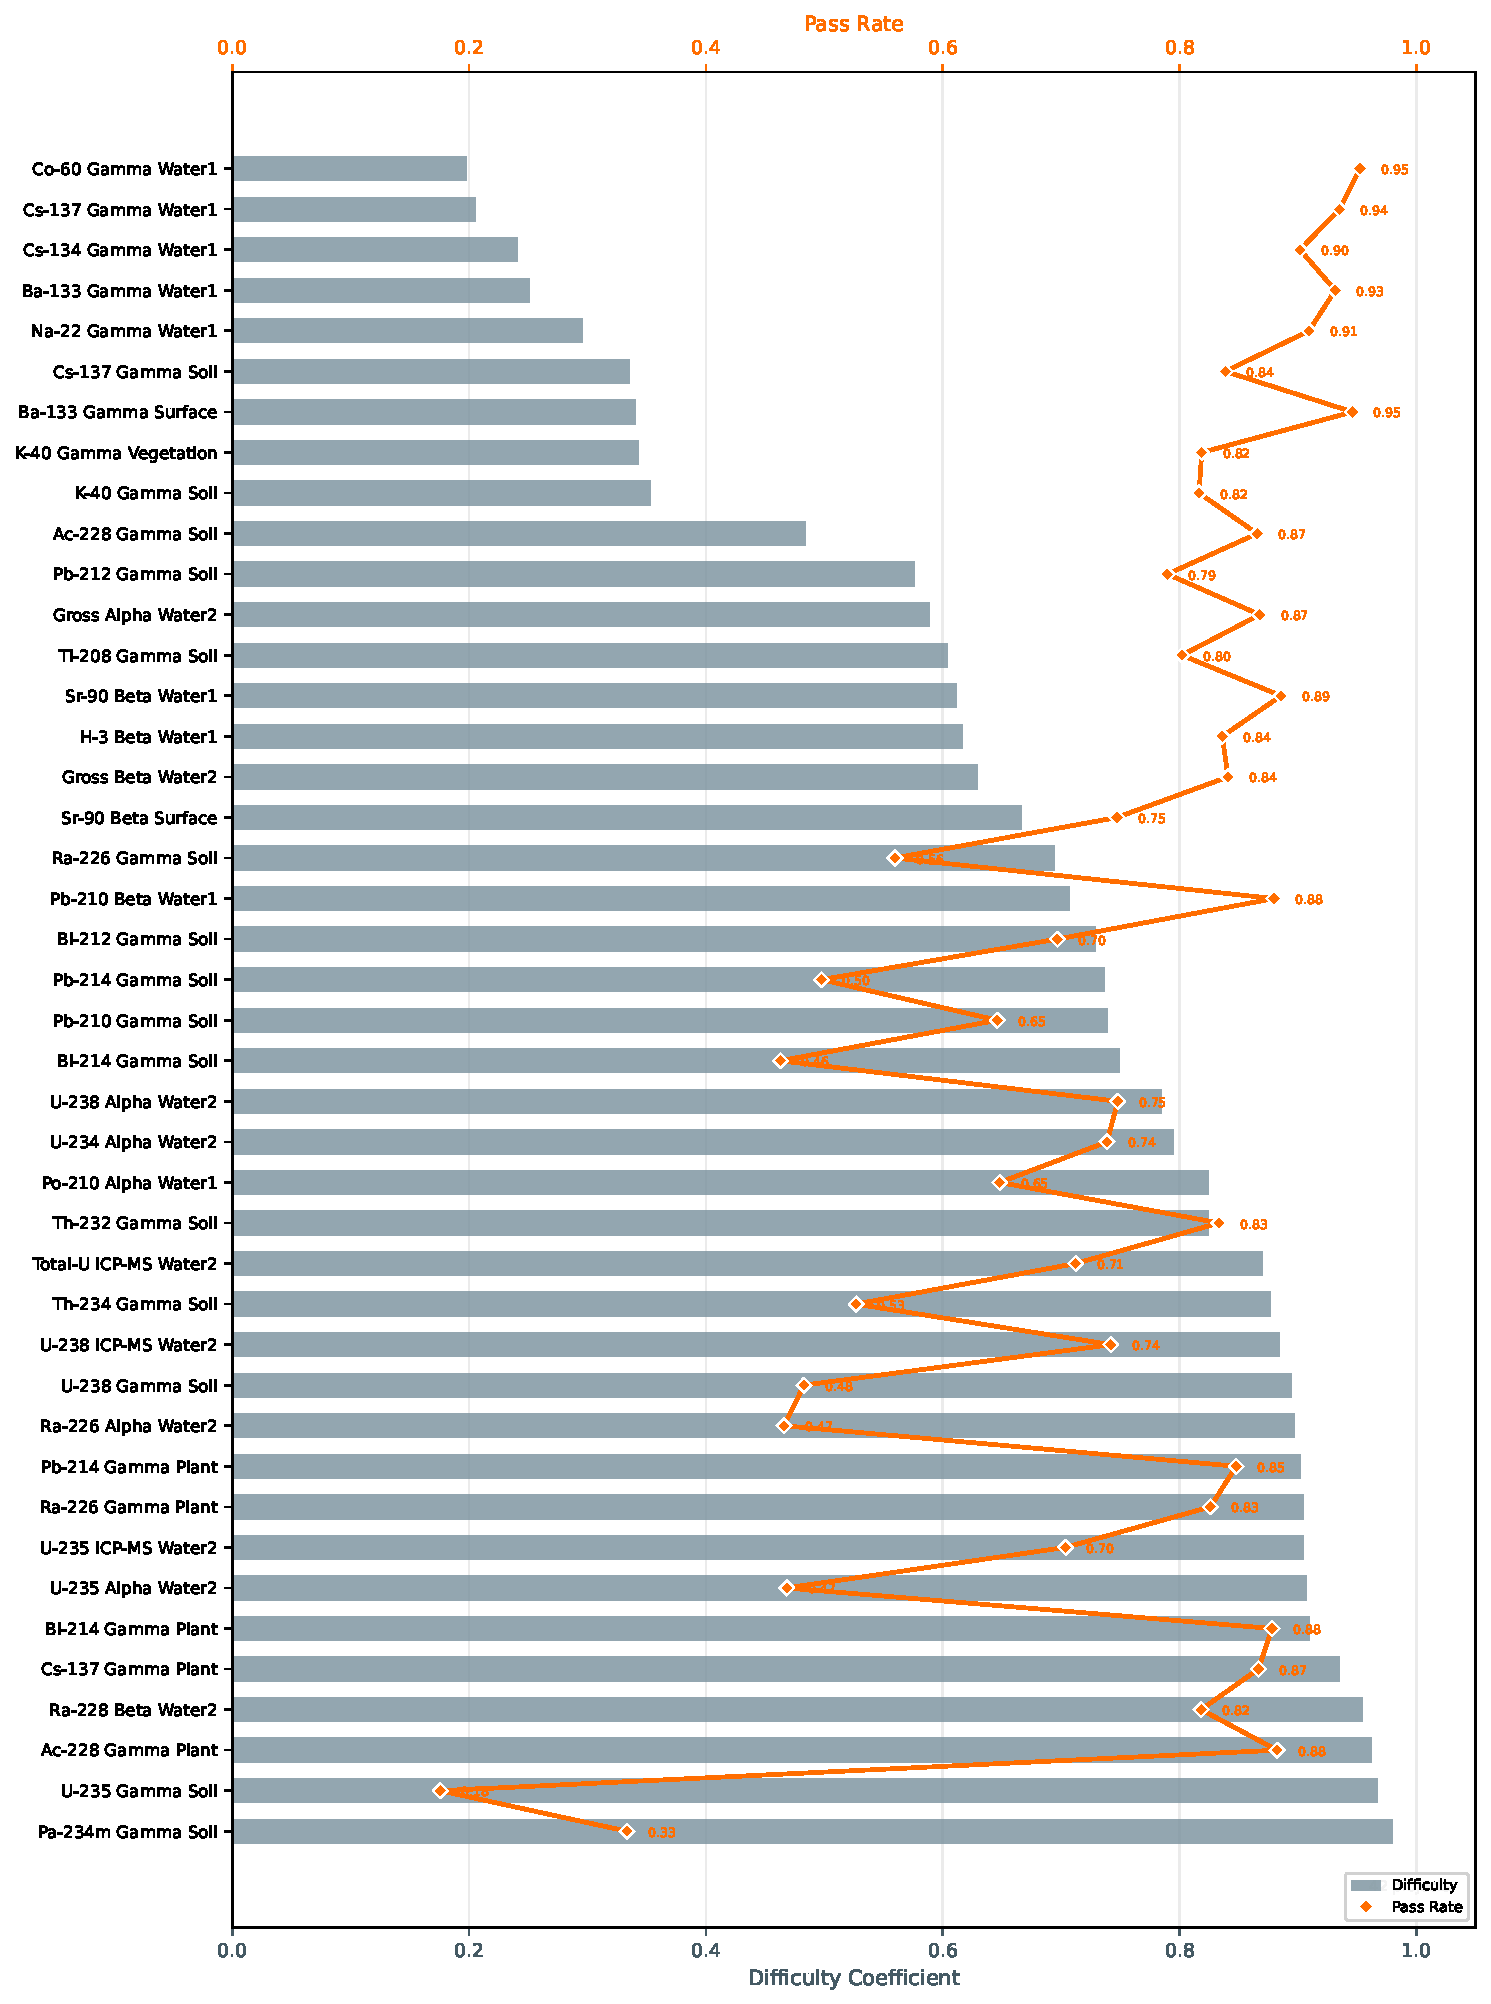
\includegraphics[width=0.68\textwidth,keepaspectratio]{../paper/figures/fig_difficulty_pass_rate_2025.pdf}};
        % Highlight top 5 water bars (ranks 1-5 out of 42, ~top 12% of figure)
        \draw[red, line width=1.8pt, rounded corners=4pt]
          ([yshift=-0.4cm]fig.north west) rectangle
          ([xshift=-0.1cm, yshift=-1.55cm]fig.north east);
      \end{tikzpicture}
    \end{column}
  \end{columns}
\end{frame}

% ===== SLIDE 7b: Bullet 2 —— 天然核素 (scattered in bottom half) =====
\begin{frame}{维度1：项目难度系数与通过率}
  \begin{columns}
    \begin{column}{0.43\textwidth}
      \small
      \begin{block}{\small 难度系数和通过率}
        \textbf{难度系数} $D_{j,y} = 1 - N^{(A)}_{j,y} / N^{\text{(all labs)}}_y$\\[1pt]
        \textbf{通过率} $P_{j,y} = N^{(A)}_{j,y} / N^{\text{(in project)}}_j$
      \end{block}
      \begin{tightitemize}
        \item \textcolor{red}{天然核素 (U同位素)}难度\textbf{最高}、通过率较低
        \item U-238, U-235 ($\alpha$/ICP-MS/$\gamma$)
        \item 活度较低，前处理与测量难度大
      \end{tightitemize}
    \end{column}
    \begin{column}{0.57\textwidth}
      \begin{tikzpicture}
        \node[anchor=north west, inner sep=0] (fig) at (0,0)
          {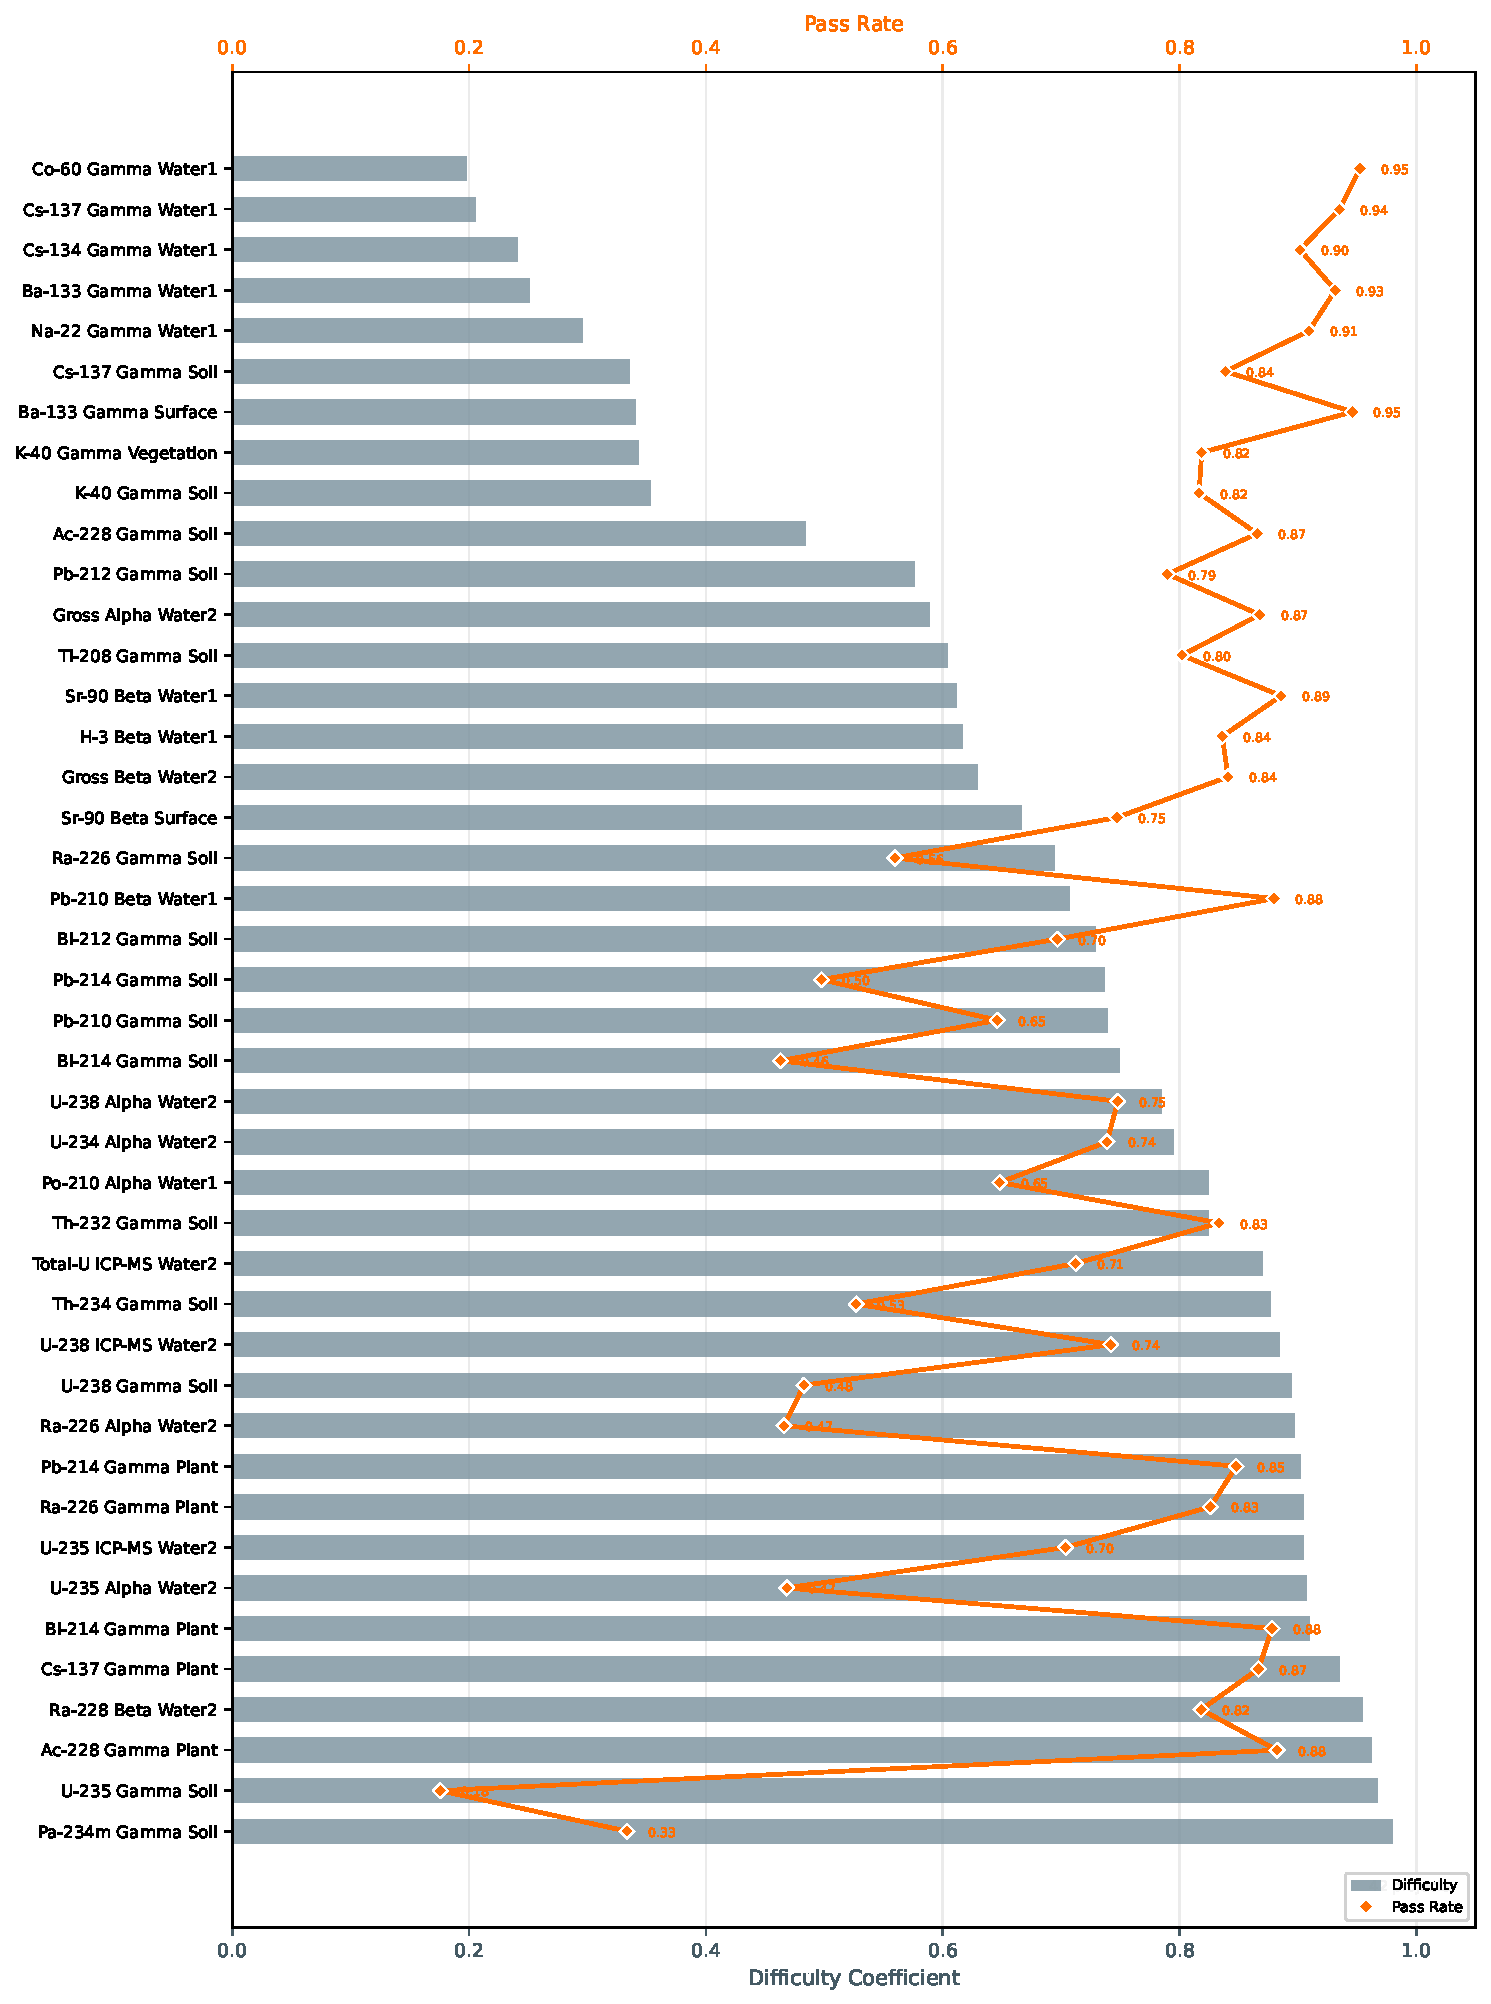
\includegraphics[width=0.68\textwidth,keepaspectratio]{../paper/figures/fig_difficulty_pass_rate_2025.pdf}};
        % Highlight bottom ~40% of figure (uranium isotopes all in bottom half)
        \draw[red, line width=1.8pt, rounded corners=4pt]
          ([yshift=-4.8cm]fig.north west) rectangle
          ([xshift=-0.1cm, yshift=2.1cm]fig.south east);
        \draw[red, line width=1.8pt, rounded corners=4pt]
          ([yshift=-5.5cm]fig.north west) rectangle
          ([xshift=-0.1cm, yshift=1.4cm]fig.south east);
        \draw[red, line width=1.8pt, rounded corners=4pt]
          ([yshift=0.9cm]fig.south west) rectangle
          ([xshift=-0.1cm, yshift=0.65cm]fig.south east);
      \end{tikzpicture}
    \end{column}
  \end{columns}
\end{frame}

% ===== SLIDE 7c: Bullet 3 —— 植物样 (scattered) =====
\begin{frame}{维度1：项目难度系数与通过率}
  \begin{columns}
    \begin{column}{0.43\textwidth}
      \small
      \begin{block}{\small 难度系数和通过率}
        \textbf{难度系数} $D_{j,y} = 1 - N^{(A)}_{j,y} / N^{\text{(all labs)}}_y$\\[1pt]
        \textbf{通过率} $P_{j,y} = N^{(A)}_{j,y} / N^{\text{(in project)}}_j$
      \end{block}
      \vspace{0.3cm}
      \begin{tightitemize}
        \item \textcolor{red}{植物样}项目难度高但通过率也高
        \item K-40, Cs-137, Ra-226, Pb-214, Bi-214 (植物)
        \item 前处理复杂，但测量本身较简单
      \end{tightitemize}
    \end{column}
    \begin{column}{0.57\textwidth}
      \begin{tikzpicture}
        \node[anchor=north west, inner sep=0] (fig) at (0,0)
          {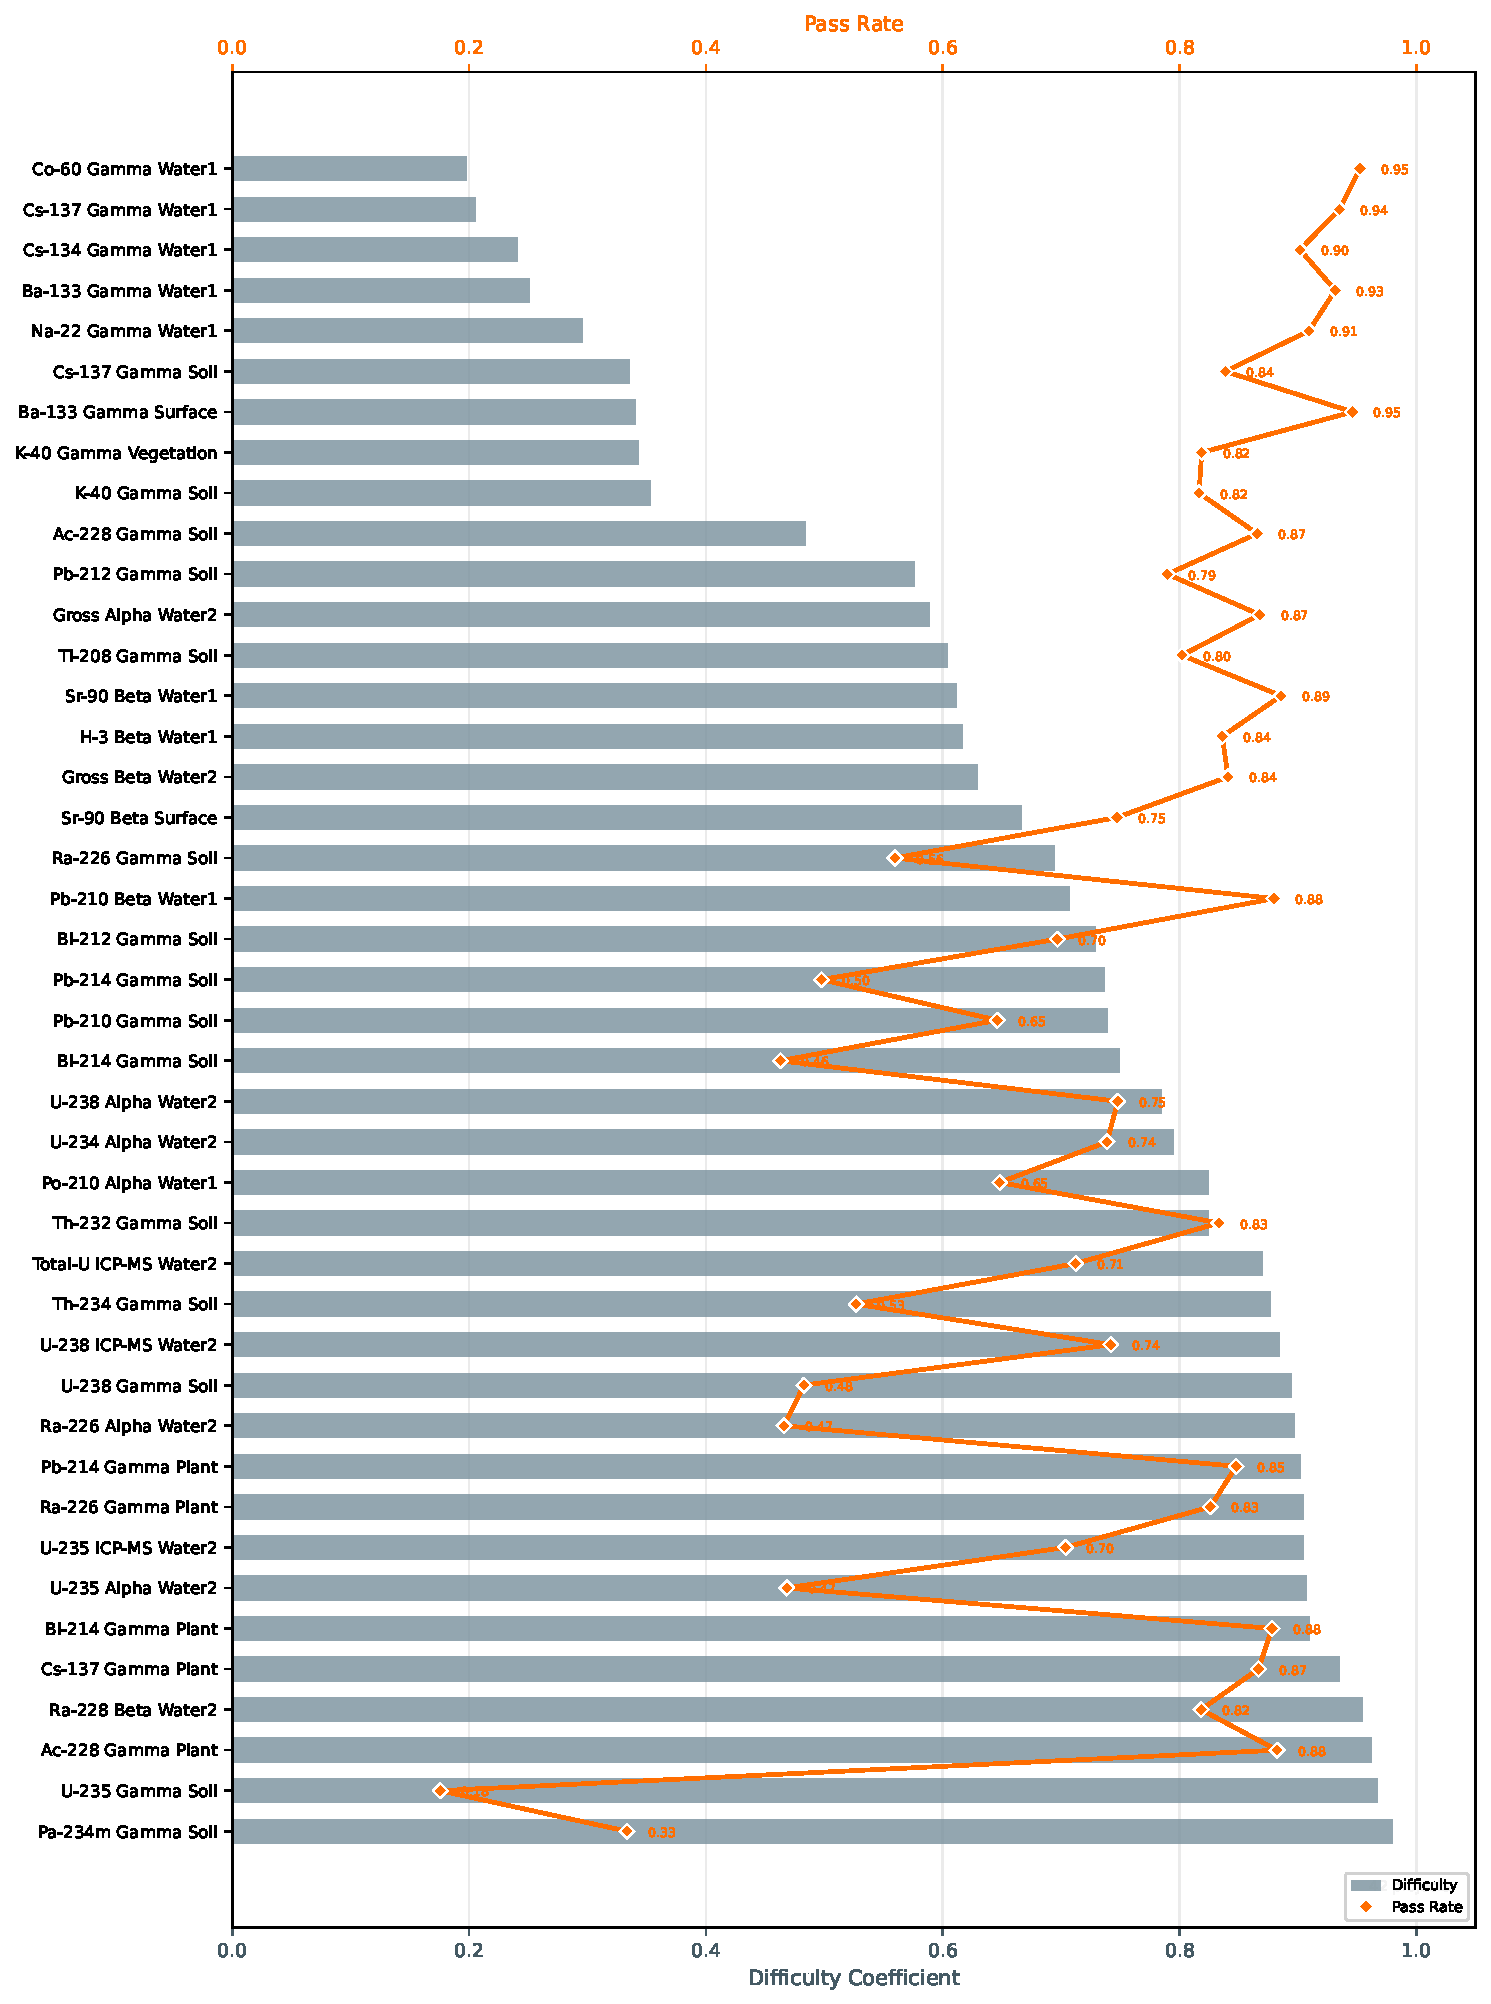
\includegraphics[width=0.68\textwidth,keepaspectratio]{../paper/figures/fig_difficulty_pass_rate_2025.pdf}};
        % Plant bars: K-40 Vegetation (~rank 8, upper), plant bars near bottom
        \draw[red, line width=1.8pt, rounded corners=4pt]
          ([yshift=-5.2cm]fig.north west) rectangle
          ([xshift=-0.1cm, yshift=1.65cm]fig.south east);
        \draw[red, line width=1.8pt, rounded corners=4pt]
          ([yshift=-5.78cm]fig.north west) rectangle
          ([xshift=-0.1cm, yshift=0.85cm]fig.south east);
      \end{tikzpicture}
    \end{column}
  \end{columns}
\end{frame}

% ===== SLIDE 7d: Bullet 4 —— 衰变链土壤 =====
\begin{frame}{维度1：项目难度系数与通过率}
  \begin{columns}
    \begin{column}{0.43\textwidth}
      \small
      \begin{block}{\small 难度系数和通过率}
        \textbf{难度系数} $D_{j,y} = 1 - N^{(A)}_{j,y} / N^{\text{(all labs)}}_y$\\[1pt]
        \textbf{通过率} $P_{j,y} = N^{(A)}_{j,y} / N^{\text{(in project)}}_j$
      \end{block}
      \vspace{0.3cm}
      \begin{tightitemize}
        \item \textcolor{red}{土壤中U--Ra衰变链}各项目通过率均较低
        \item U-238 $\to$ Th-234 $\to$ Pa-234m $\to$ \dots $\to$ Ra-226 $\to$ \dots $\to$ Pb-214 $\to$ Bi-214
        \item 未达长期平衡或者未密封好导致氡气泄漏
      \end{tightitemize}
    \end{column}
    \begin{column}{0.57\textwidth}
      \begin{tikzpicture}
        \node[anchor=north west, inner sep=0] (fig) at (0,0)
          {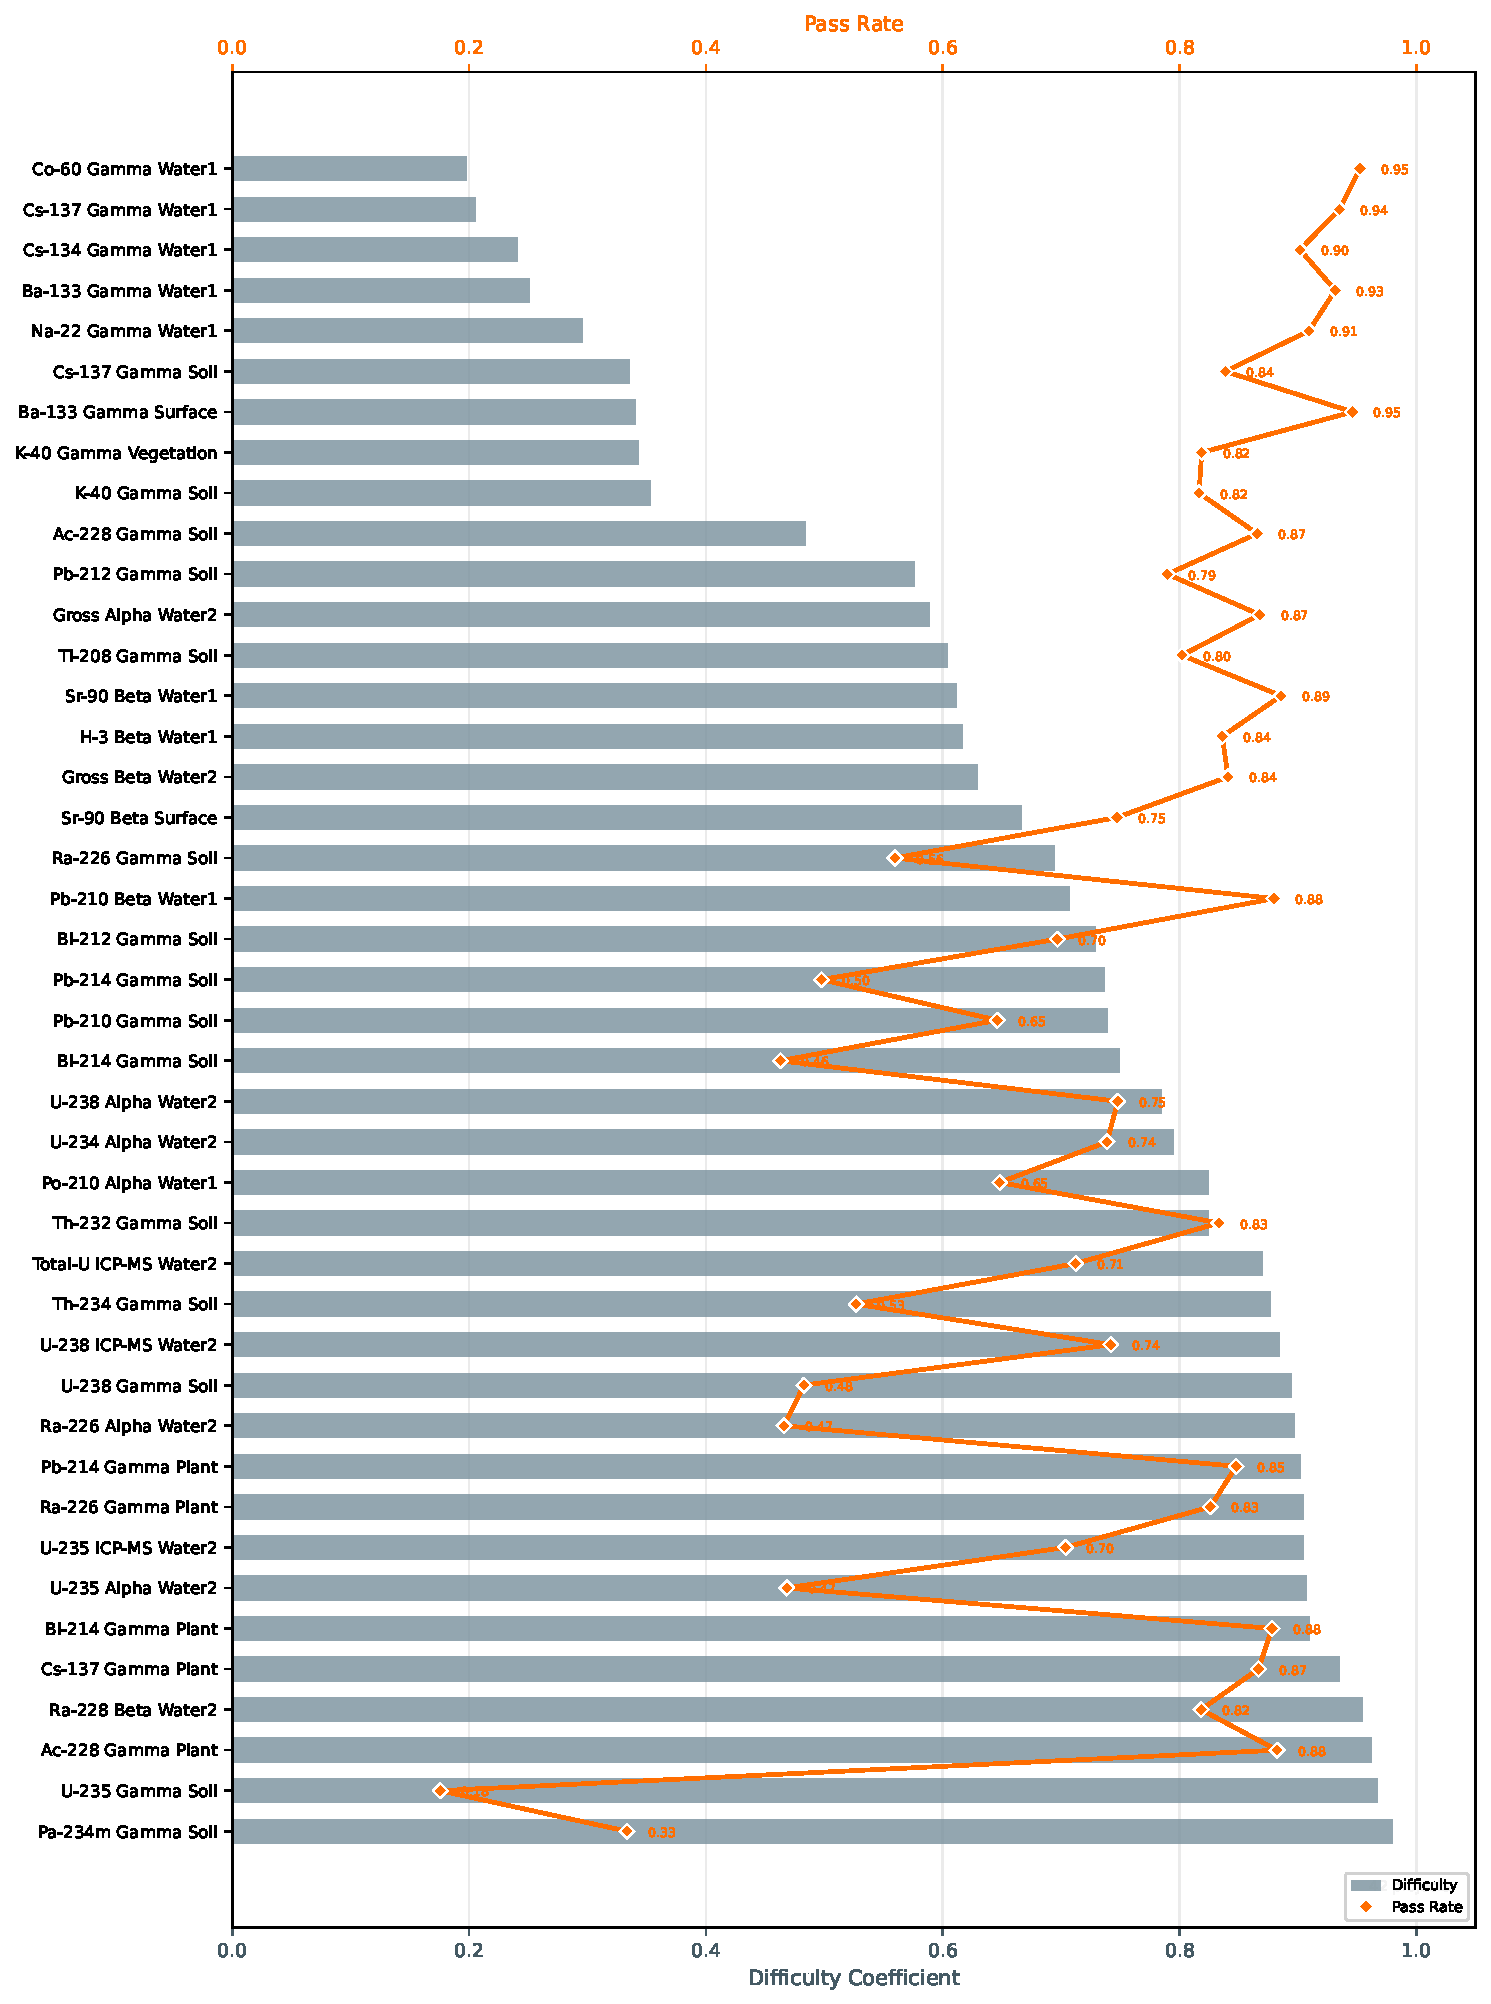
\includegraphics[width=0.68\textwidth,keepaspectratio]{../paper/figures/fig_difficulty_pass_rate_2025.pdf}};
        % Decay chain soil bars scattered: U-238,Th-234 soil (~rank 17-18, upper-mid),
        % Pa-234m soil (~rank 40, near bottom), Ra-226,Pb-214,Bi-214 soil (ranks 20-25, mid-lower)
        \draw[red, line width=1.8pt, rounded corners=4pt]
          ([yshift=-3.0cm]fig.north west) rectangle
          ([xshift=-1.7cm, yshift=3.27cm]fig.south east);
        \draw[red, line width=1.8pt, rounded corners=4pt]
          ([yshift=-4.6cm]fig.north west) rectangle
          ([xshift=-1.7cm, yshift=2.1cm]fig.south east);
        \draw[red, line width=1.8pt, rounded corners=4pt]
          ([yshift=0.8cm]fig.south west) rectangle
          ([xshift=-1.7cm, yshift=0.55cm]fig.south east);
      \end{tikzpicture}
    \end{column}
  \end{columns}
\end{frame}

% ===== SLIDE 5: 难度 =====
\begin{frame}{维度2：项目难度随时间变化趋势}
  \begin{columns}
    \begin{column}{0.48\textwidth}
      \centering
      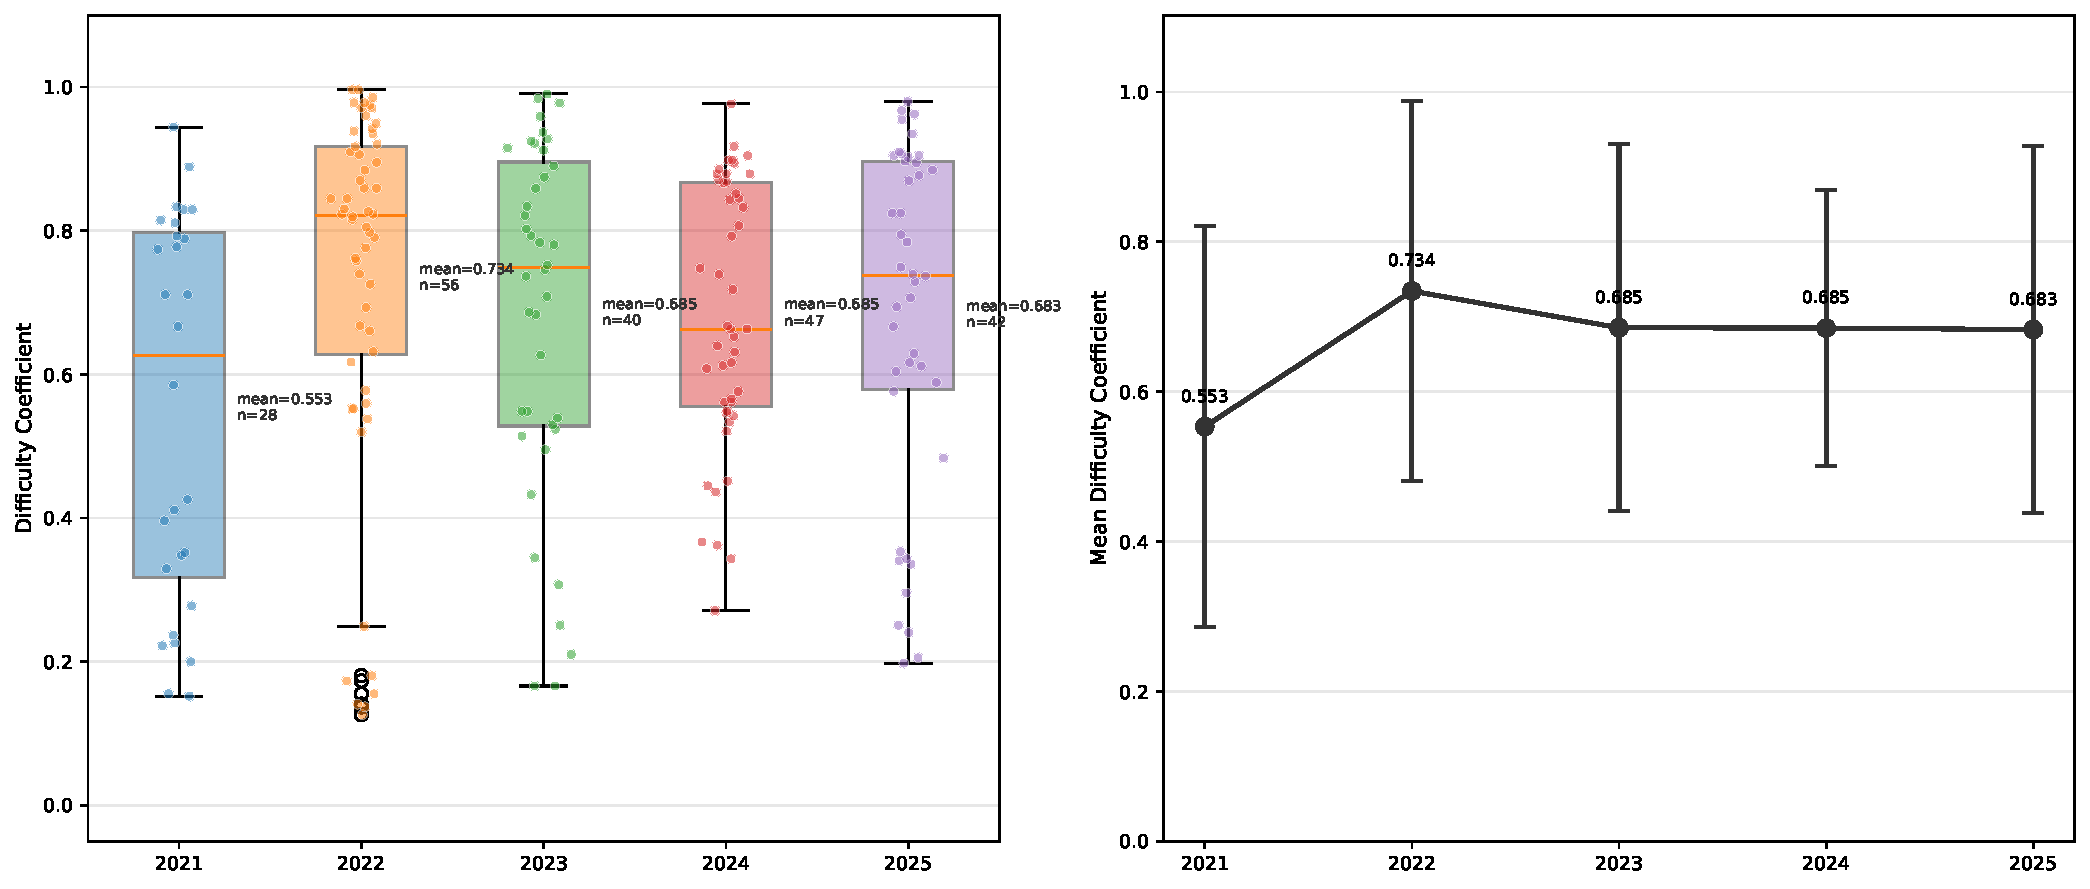
\includegraphics[width=\textwidth,height=5cm,keepaspectratio]{../paper/figures/fig_difficulty_overview.pdf}\\[2pt]
      {\scriptsize (a) 各年难度分布 (b) 均值$\pm$1$\sigma$}
      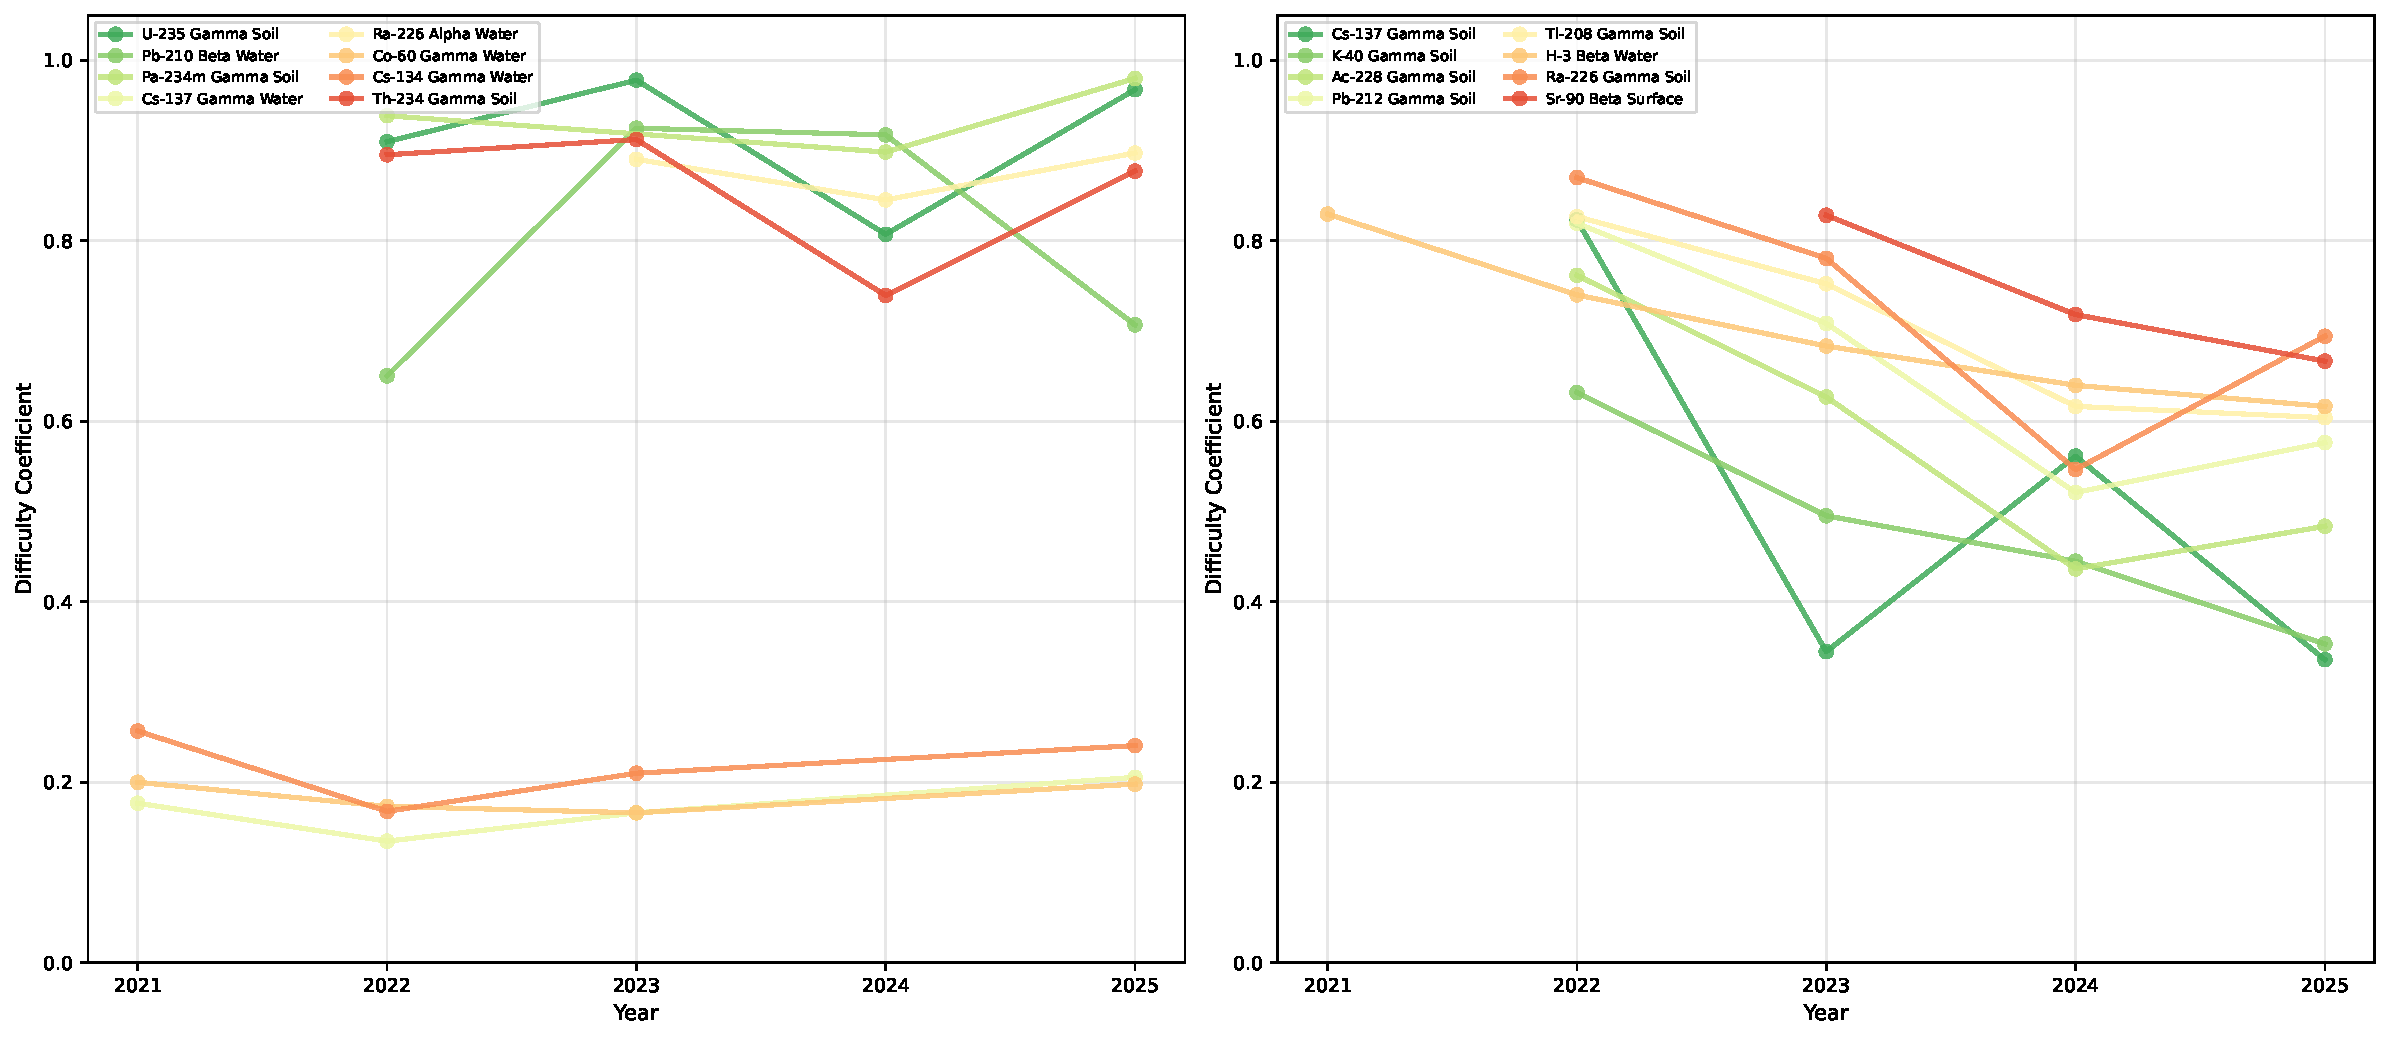
\includegraphics[width=\textwidth,height=4.8cm,keepaspectratio]{../paper/figures/fig_difficulty_trends.pdf}\\[2pt]
      {\scriptsize 难度变化增加最多的项目（左图）和减少最多的项目（右图） ($\geq 3$年)}
      \small
    \end{column}
    \begin{column}{0.48\textwidth}
      \centering
      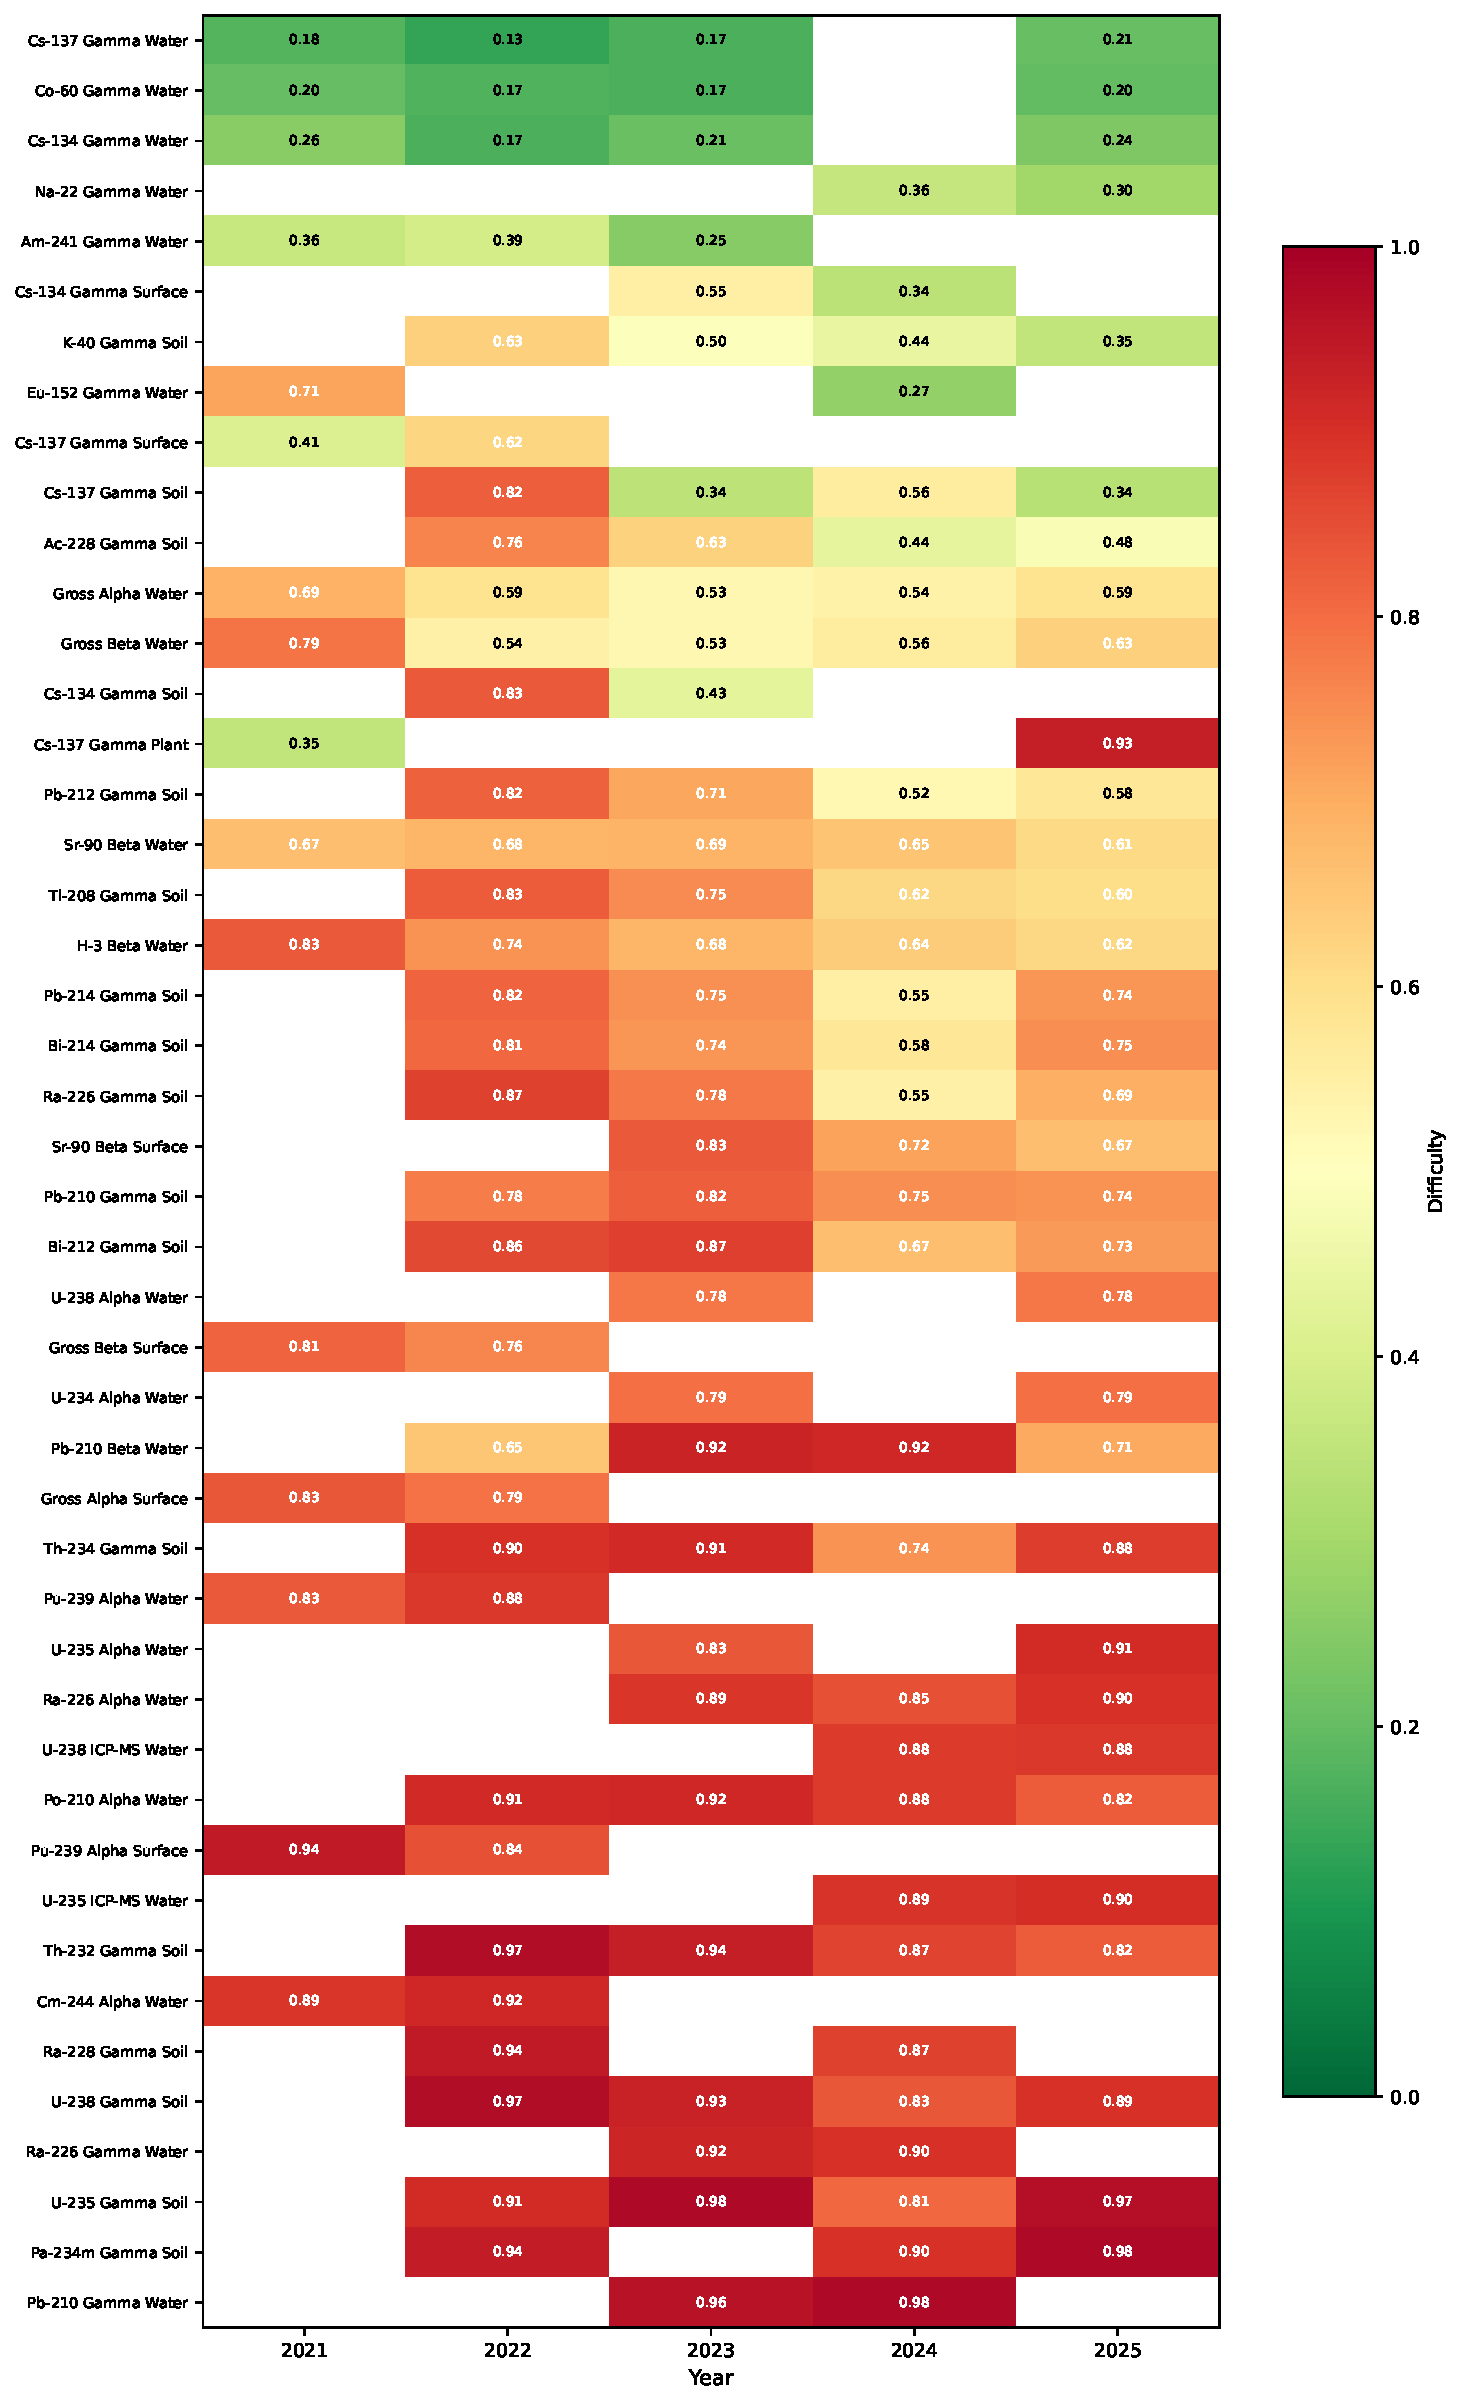
\includegraphics[width=0.60\textwidth,keepaspectratio]{../paper/figures/fig_difficulty_heatmap.pdf}\\[2pt]
      {\scriptsize 多年项目难度热力图 (绿=容易, 红=困难)}
    \end{column}
  \end{columns}
\end{frame}


% ===== SLIDE 7: 实验室表现 =====
\begin{frame}{维度2：实验室间比对排名}
  \begin{columns}
    \begin{column}{0.50\textwidth}
      \centering
      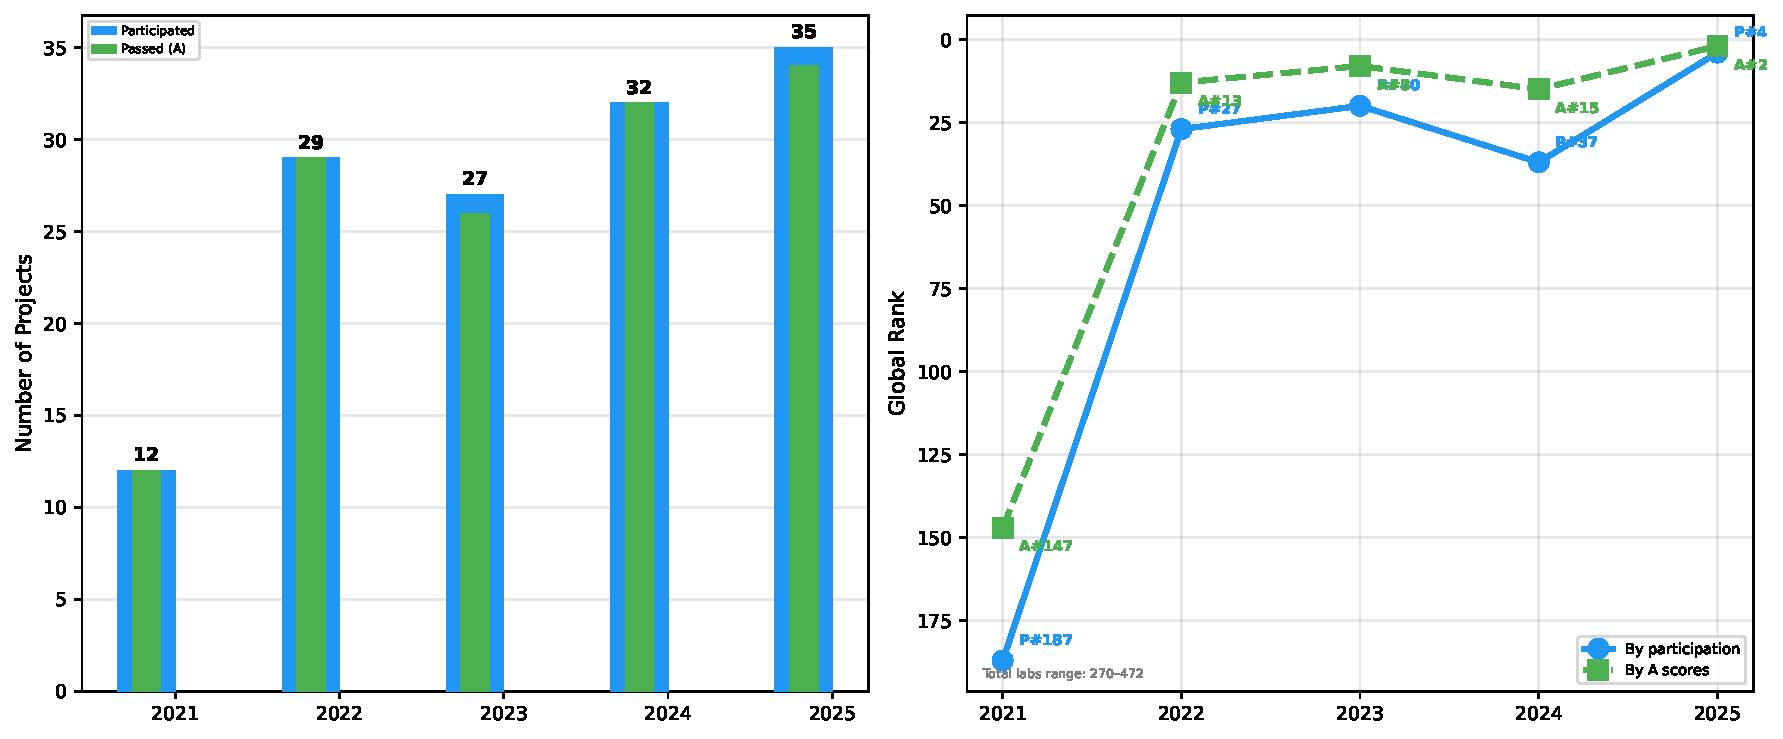
\includegraphics[width=\textwidth,height=5.2cm,keepaspectratio]{../paper/figures/fig_lab_performance.pdf}\\[2pt]
      {\scriptsize (a) 年度参与/通过数\quad (b) 全球排名}
      \vspace{0.15cm}
      \small
      \begin{tightitemize}
        \item 参与：\#187/270 $\to$ \#4/399；
	\item A计数：\#147/270 $\to$\#2/399
        \item 总通过率 98.5\% (133/135)，零N结果
	\item 两个W结果（2023年"Sr90 Beta Surface3"和2025年"U235 Alpha Water")：精度未达标
      \end{tightitemize}
    \end{column}
    \begin{column}{0.50\textwidth}
      \centering
      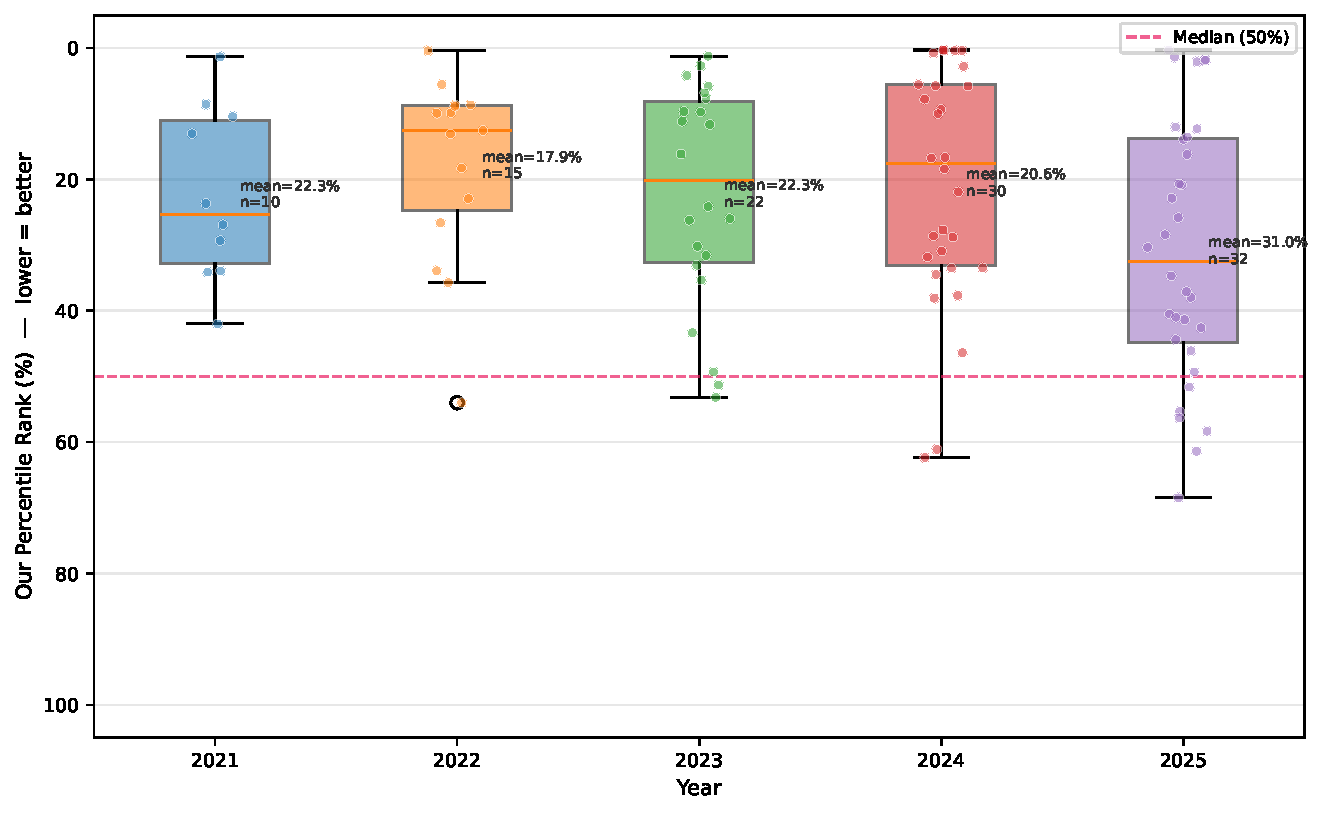
\includegraphics[width=\textwidth,height=5.2cm,keepaspectratio]{../paper/figures/fig_lab_percentile_ranking.pdf}\\[2pt]
      {\scriptsize 项目内百分位排名 (按照相对偏差排序，排名越靠前越好)}
      \vspace{0.15cm}
      \small
      \begin{tightitemize}
        \item 历年均值 23.8\% (95\% CI: 20.4--27.2\%)
        \item Wilcoxon test: $p{<}0.001$ (109个项目中，97个项目的|RB|显著低于同行中位数)
      \end{tightitemize}
    \end{column}
  \end{columns}
\end{frame}

% ===== SLIDE 8: 分层 =====
\begin{frame}{维度4：难度分层分析}
  \begin{columns}   
 \begin{column}{0.48\textwidth}
      \centering
      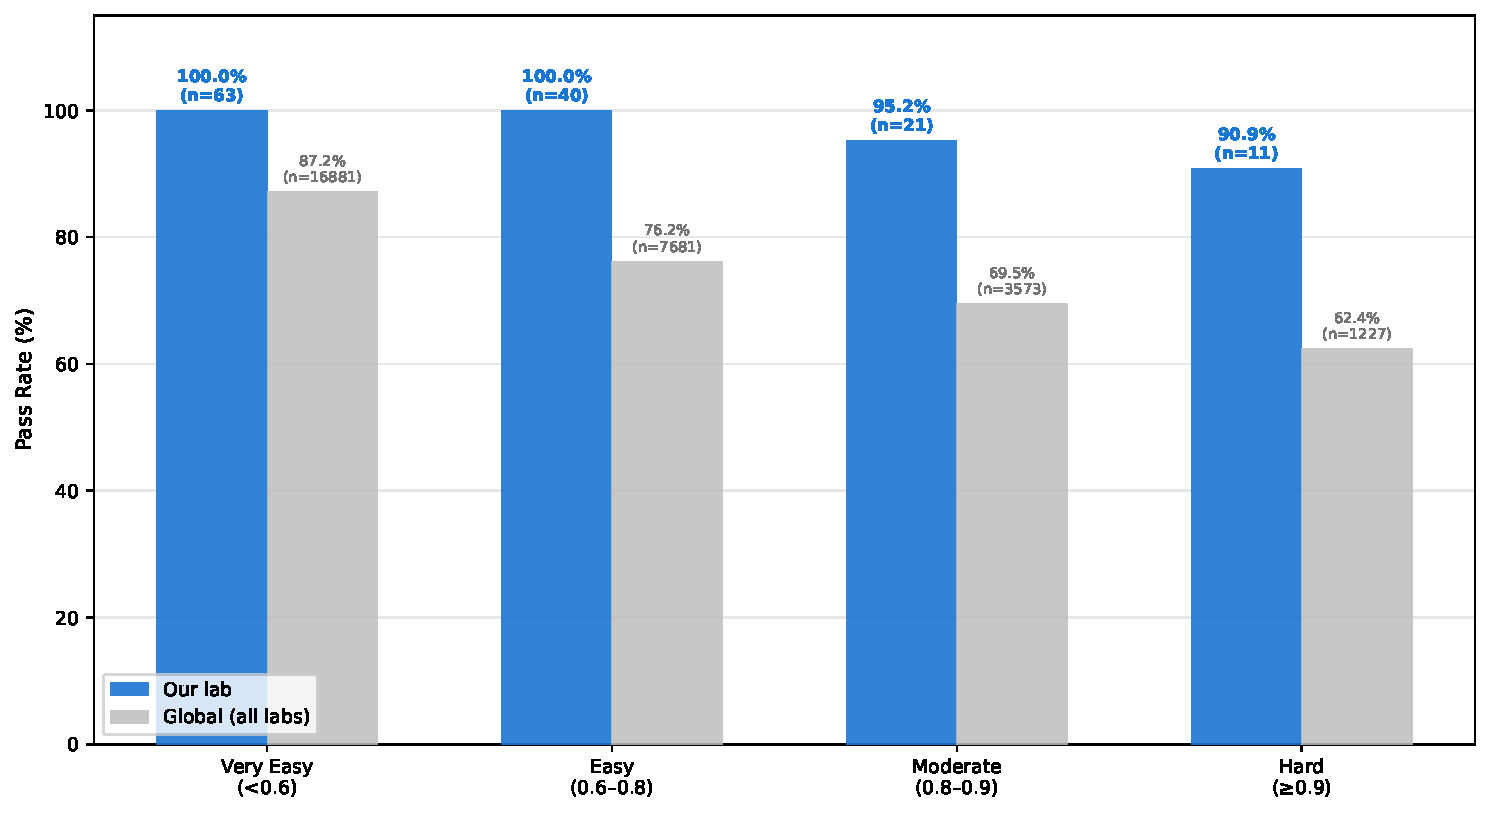
\includegraphics[width=\textwidth,height=4.8cm,keepaspectratio]{../paper/figures/fig_difficulty_tier_pass_rate.pdf}\\[2pt]
      {\scriptsize 通过率：本单位 vs. 全球均值}
    \end{column}
    \begin{column}{0.48\textwidth}
      \centering
      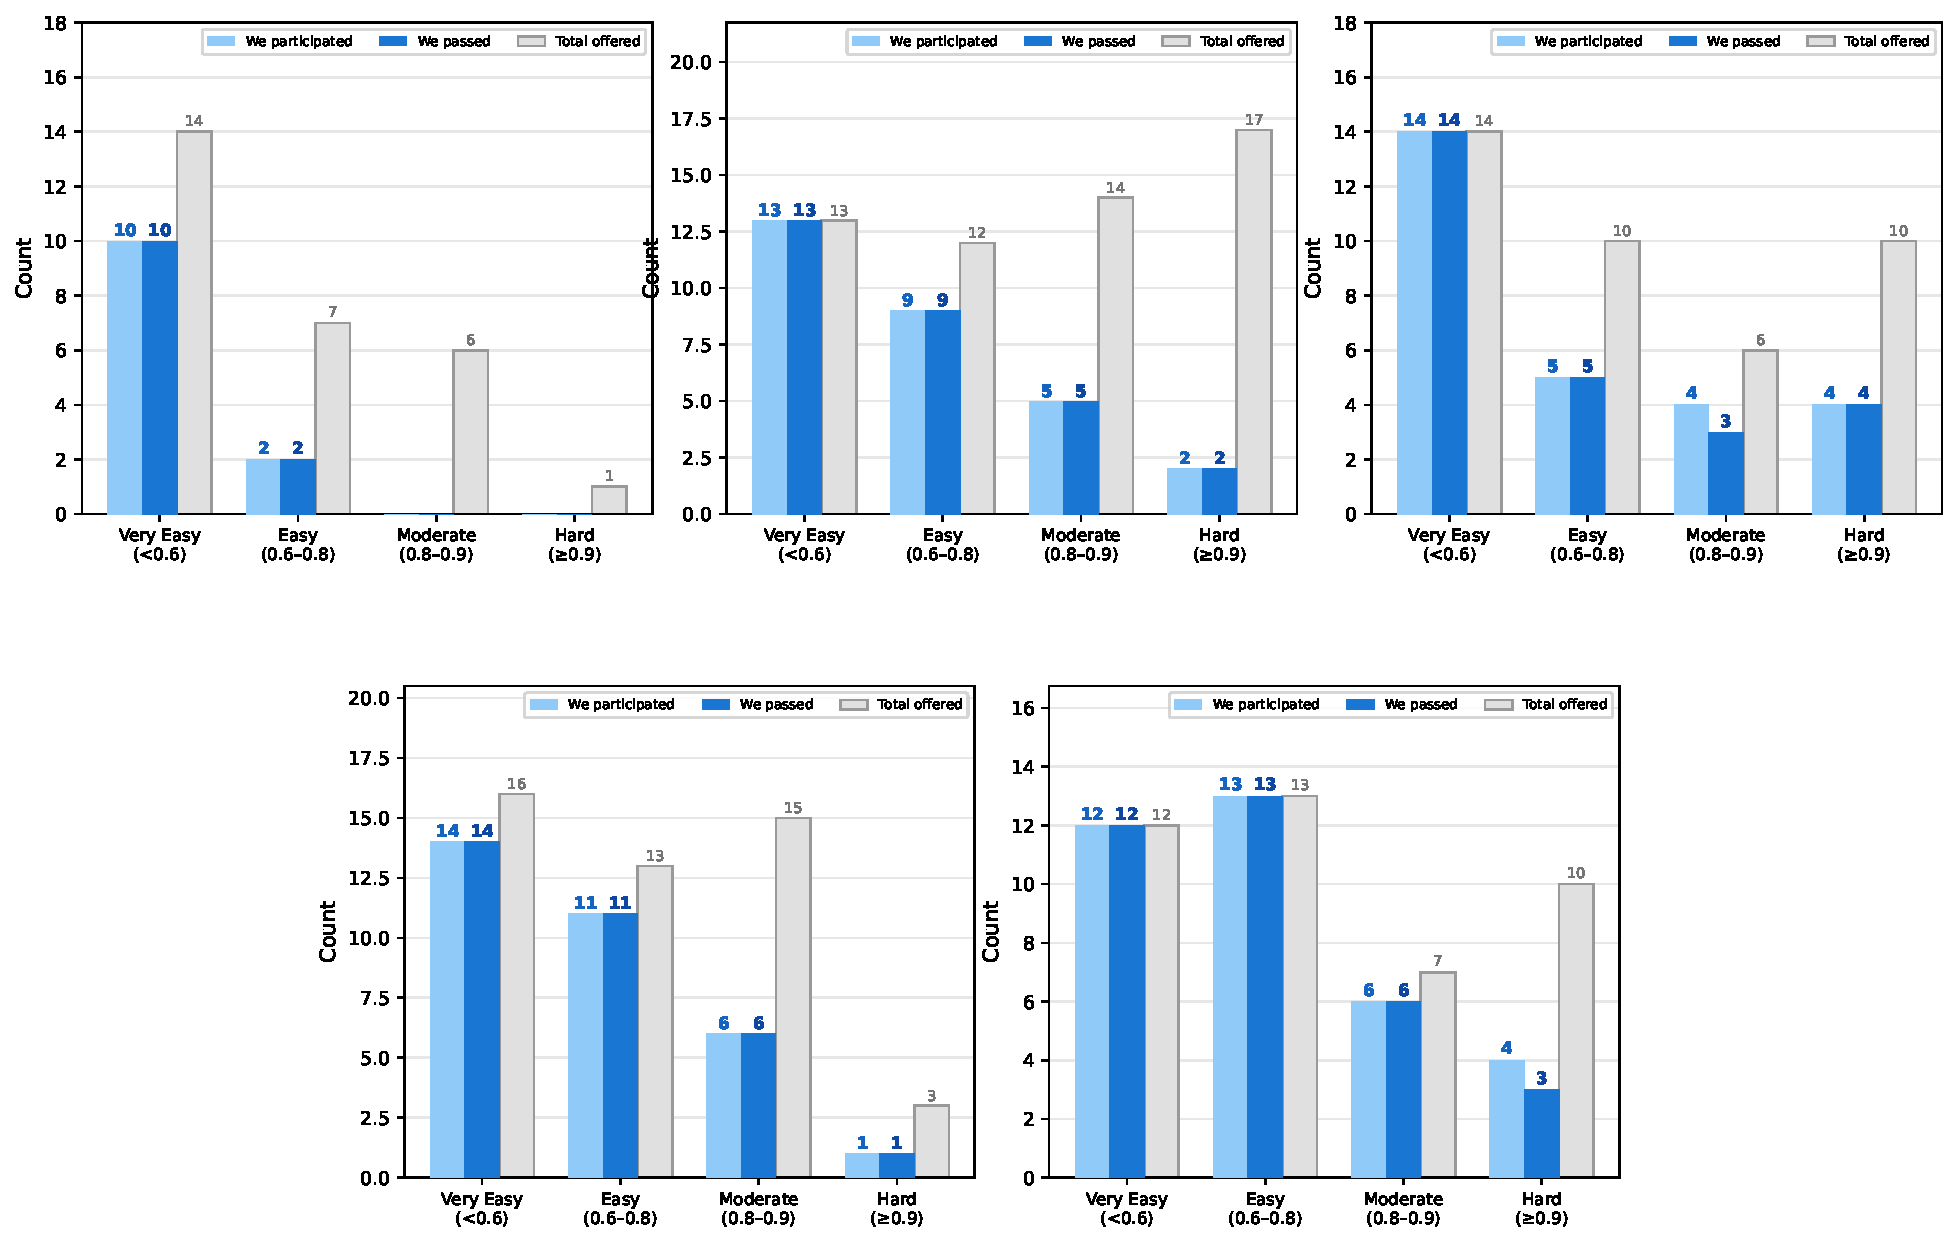
\includegraphics[width=\textwidth,height=4.8cm,keepaspectratio]{../paper/figures/fig_difficulty_tier_counts.pdf}\\[2pt]
      {\scriptsize 各年各层级项目数}
    \end{column}
  \end{columns}
  \vspace{0.1cm}
  \centering\small
  \begin{tabular}{@{}lcccc@{}}
    \toprule
    \textbf{层级} & \textbf{Very Easy ($D{<}0.6$)} & \textbf{Easy (0.6--0.8)} & \textbf{Moderate (0.8--0.9)} & \textbf{Hard ($D{>}0.9$)} \\
    \midrule
    本单位 & 100\% & 100\% & 95.0\% (19/20) & \textbf{91.7\% (11/12)} \\
    全球 & 87.2\% (86.7--87.7) & 76.2\% (75.2--77.2) & 69.4\% (67.8--70.9) & 63.2\% (60.6--65.8) \\
    \bottomrule
  \end{tabular}
  \par{\small 括号内为95\% 置信区间。本单位在各层级均显著优于全球均值。}
\end{frame}


% ===== SLIDE 10: 偏差 =====
\begin{frame}{维度5：相对偏差与项目内排名}
  \begin{columns}
    \begin{column}{0.48\textwidth}
      \centering
      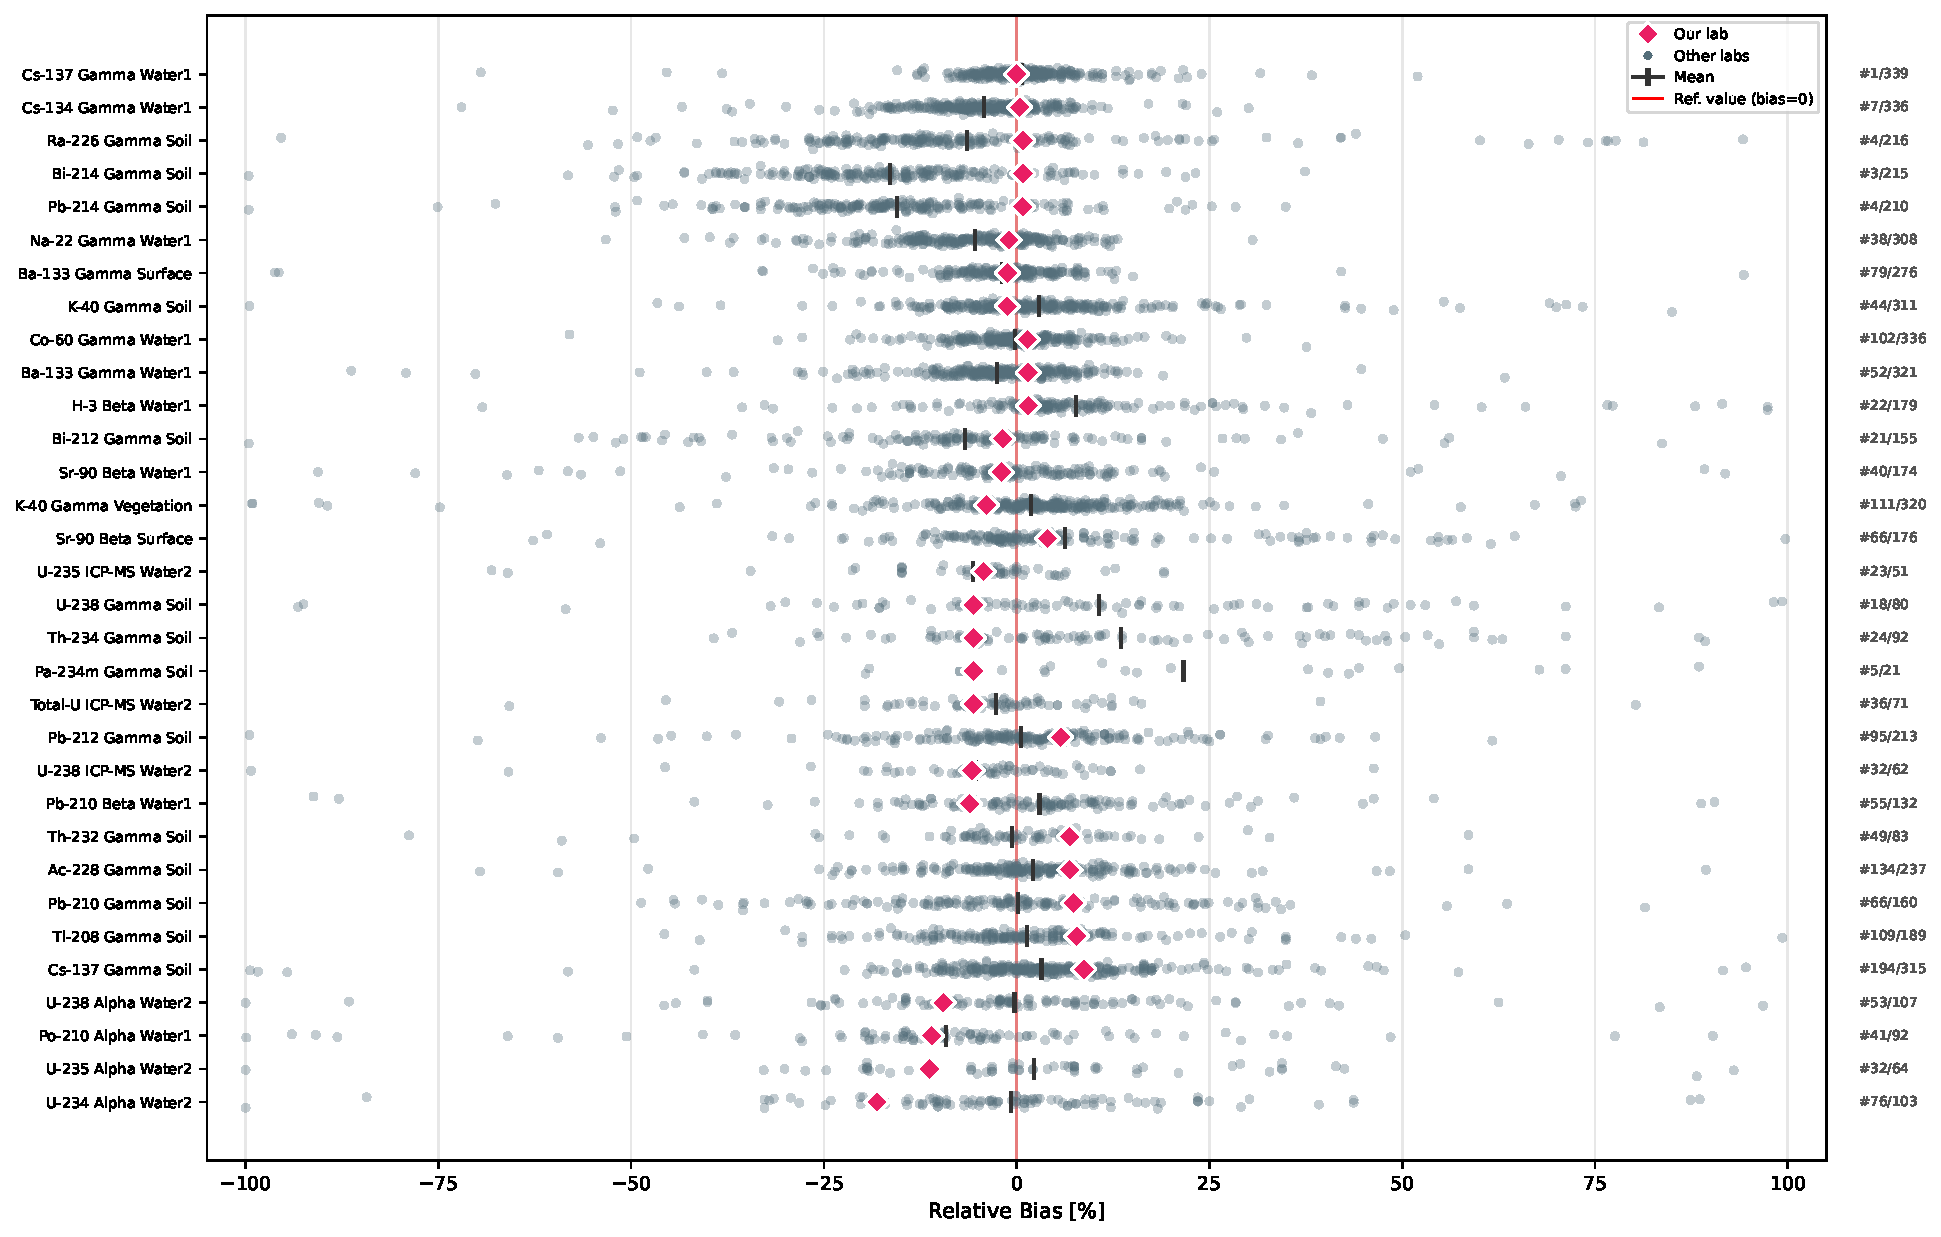
\includegraphics[width=\textwidth,height=5cm,keepaspectratio]{../paper/figures/fig_relative_bias_2025.pdf}\\[2pt]
      {\scriptsize 2025年项目内相对偏差分布}
      \vspace{0.15cm}
      \small
      \begin{tightitemize}
        \item 63.6\%项目偏差优于同行均值
        \item 最优:  ${}^{137}$Cs 水 \#1/339；最弱: ${}^{234}$U ($\alpha$)
	\item ${}^{226}\text{Ra}$, ${}^{214}\text{Pb}$, ${}^{214}\text{Bi}$ 测量结果普遍偏低
      \end{tightitemize}
    \end{column}
    \begin{column}{0.48\textwidth}
      \centering
      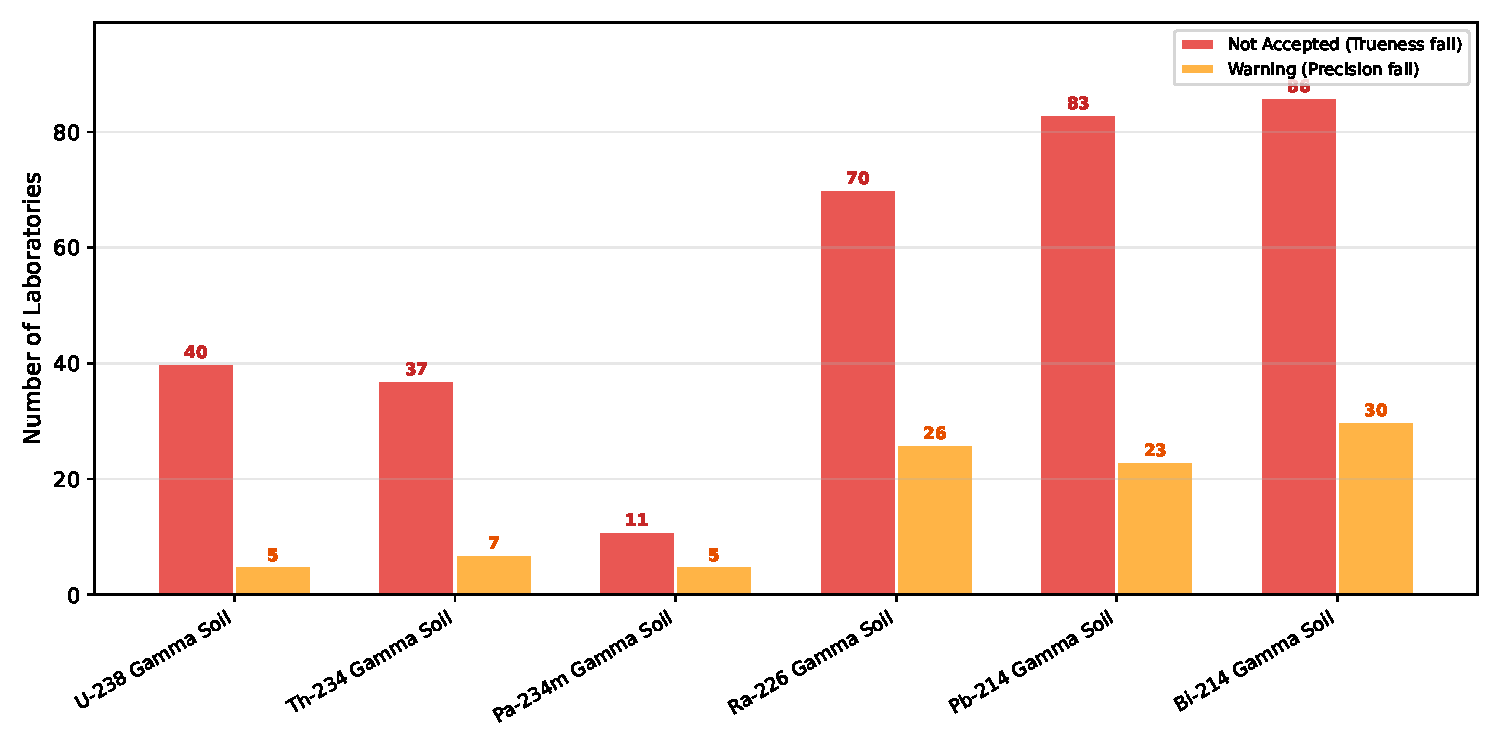
\includegraphics[width=\textwidth,height=5cm,keepaspectratio]{../paper/figures/fig_decay_chain_nw_breakdown.pdf}
      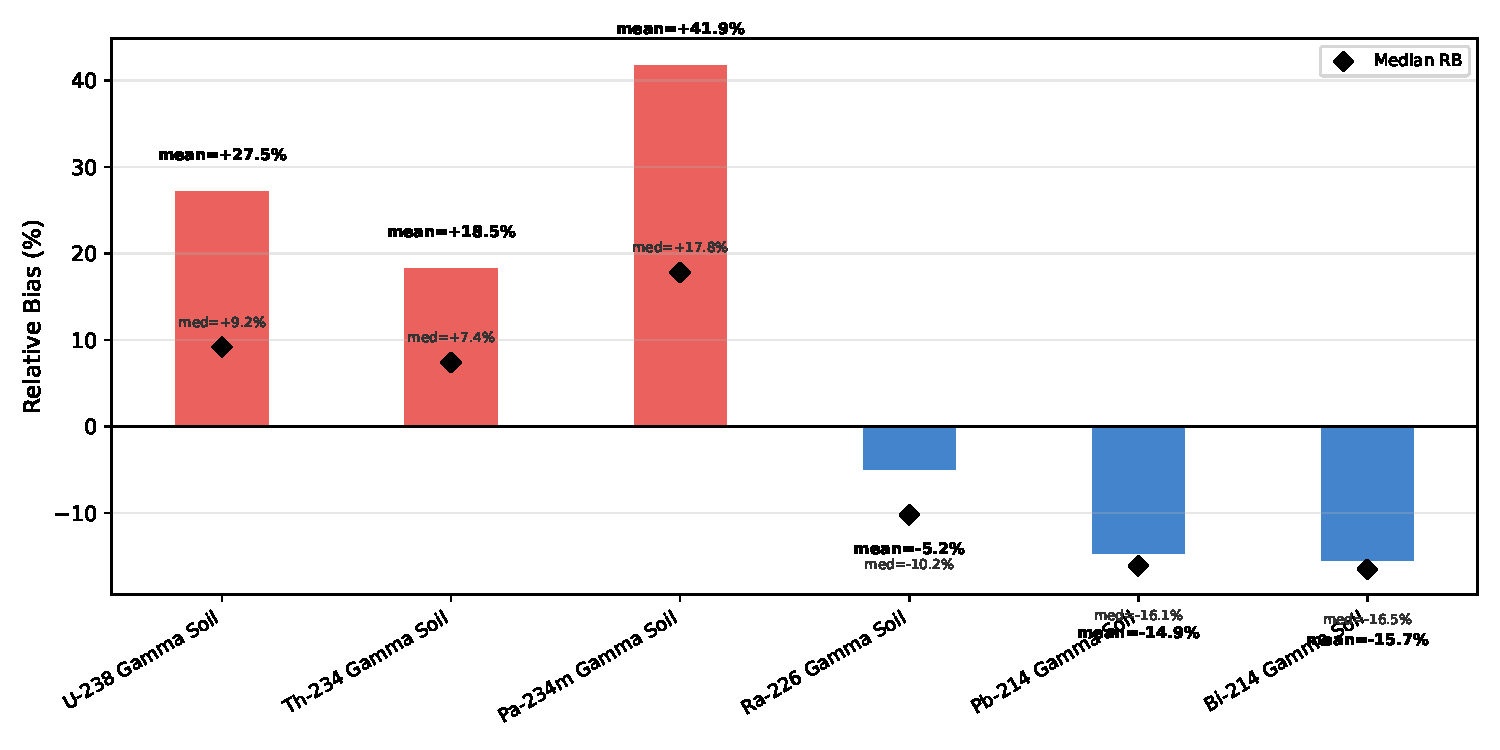
\includegraphics[width=\textwidth,height=5cm,keepaspectratio]{../paper/figures/fig_decay_chain_bias_direction.pdf}
    \end{column}
  \end{columns}
\end{frame}


% ===== SLIDE 12: 局限 =====
\begin{frame}{局限性与实际意义}
  \small
  \begin{columns}
    \begin{column}{0.45\textwidth}
      \begin{block}{\small 局限性}
        \begin{tightenumerate}
          \item 难度系数 $D$ 有可能混淆参与广度与内在难度
          \item 单实验室案例，可推广性待验证
          \item 更长时间维度可以增强说服力
        \end{tightenumerate}
      \end{block}
    \end{column}
    \begin{column}{0.55\textwidth}
      \begin{block}{\small 实际意义}
        \begin{tightitemize}
	\item 项目难度分级，通过多维比较找到易错项目并剖析原因
          \item 难度分层排除"只挑简单项目"的质疑
          \item 框架模块化、代码公开，其他实验室可直接复用
        \end{tightitemize}
      \end{block}
    \end{column}
  \end{columns}
      \vspace{0.2cm}
      \centering\textcolor{mainblue}{\small\texttt{github.com/yunlongli15/iaea-pt-analysis-2021-2025}}
\end{frame}

% ===== SLIDE 13: 结论 =====
\begin{frame}{结论}
  \small
  \begin{tightenumerate}
    \item \textbf{多维度框架}将传统A/W/N报告扩展为五维分析，提供更丰富的实验室性能画像
    \vspace{0.1cm}
    \item 本实验室2025年获得满意项目个数位居全球前列；Wilcoxon检验确认准确度显著优于同行中位数 ($p{<}0.001$)
    \vspace{0.1cm}
    \item \textbf{难度分层}表明即使在Hard层级仍维持91.7\%通过率，远超全球均值63.2\%
    \vspace{0.1cm}
    \item \textbf{统计推断}为描述性发现提供关键限定：5年趋势不显著
    \vspace{0.1cm}
    \item 框架模块化、代码公开，可作为其他实验室的\textcolor{accent}{PT自评估模板}
  \end{tightenumerate}
\end{frame}

% ===== SLIDE 14: 致谢 =====
{
\setbeamertemplate{background}{
  \begin{tikzpicture}[remember picture,overlay]
    \fill[mainblue] (current page.south west) rectangle (current page.north east);
  \end{tikzpicture}
}
\begin{frame}
  \color{white}\centering
  \vspace{2cm}
  {\Huge\bfseries 谢谢！}\\[1cm]
  {\Large 欢迎提问}
\end{frame}
}

% ===================================================================
% APPENDIX
% ===================================================================
\appendix

% --- Backup 1a: Difficulty 2021-2022 ---
{
\begin{frame}[plain]{备用：各年度难度与通过率 (2021--2022)}
  \centering
  \begin{columns}
    \begin{column}{0.48\textwidth}
      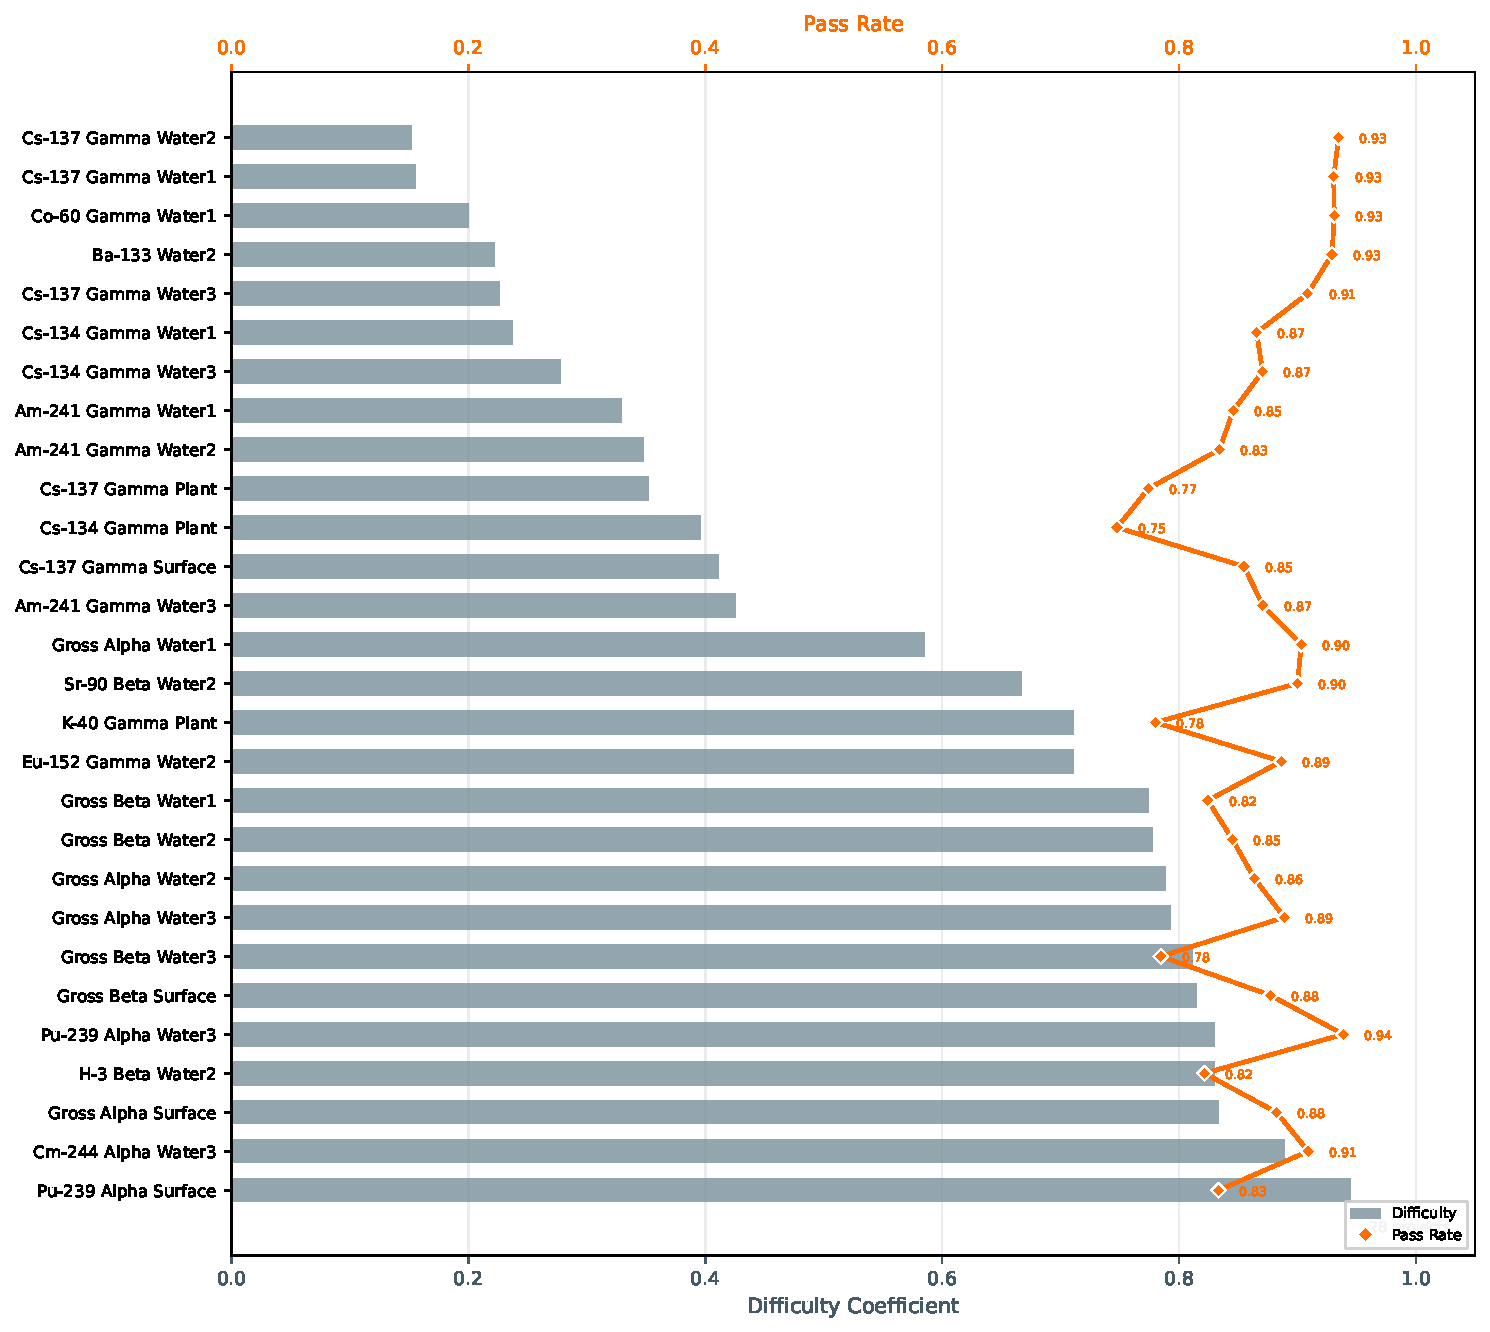
\includegraphics[width=\textwidth,height=7cm,keepaspectratio]{../paper/figures/fig_difficulty_pass_rate_2021.pdf}\\[2pt]{\small 2021: 28项目, $\bar{D}{=}0.553$}
    \end{column}
    \begin{column}{0.48\textwidth}
      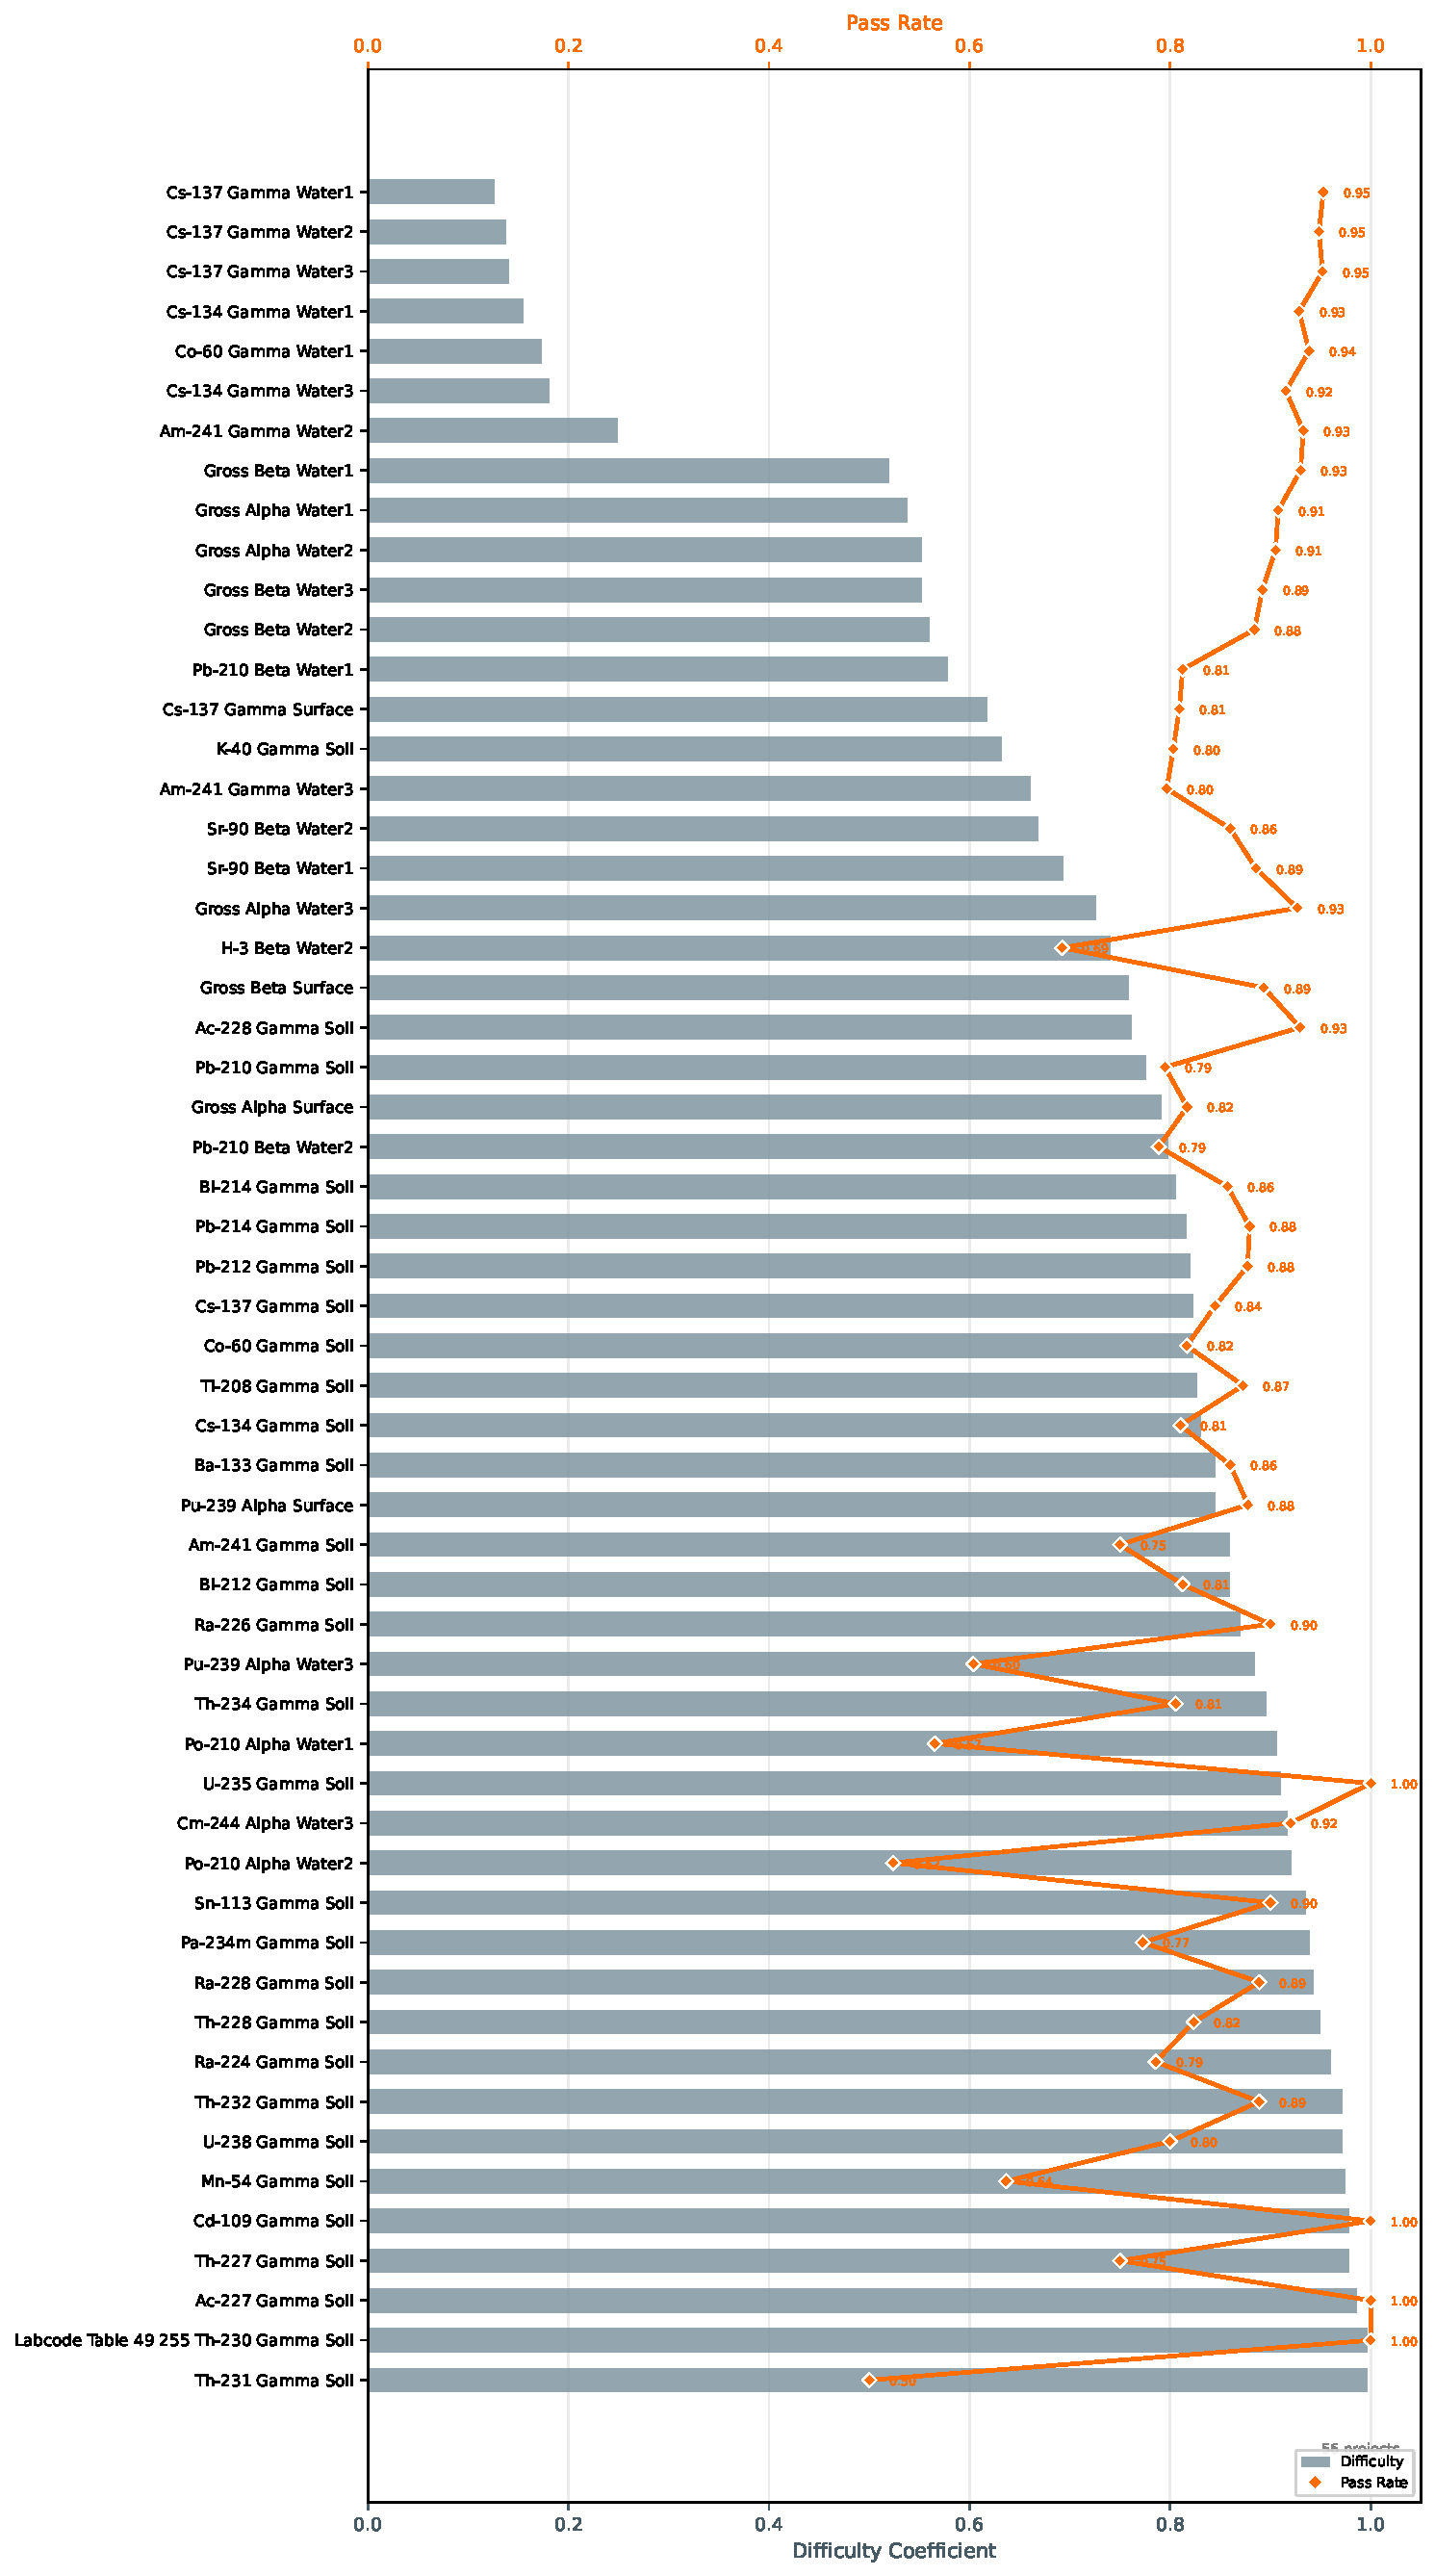
\includegraphics[width=\textwidth,height=6cm,keepaspectratio]{../paper/figures/fig_difficulty_pass_rate_2022.pdf}\\[2pt]{\small 2022: 56项目, $\bar{D}{=}0.734$}
    \end{column}
  \end{columns}
\end{frame}
}

% --- Backup 1b: Difficulty 2023-2024 ---
{
\begin{frame}[plain]{备用：各年度难度与通过率 (2023--2024)}
  \centering
  \begin{columns}
    \begin{column}{0.48\textwidth}
      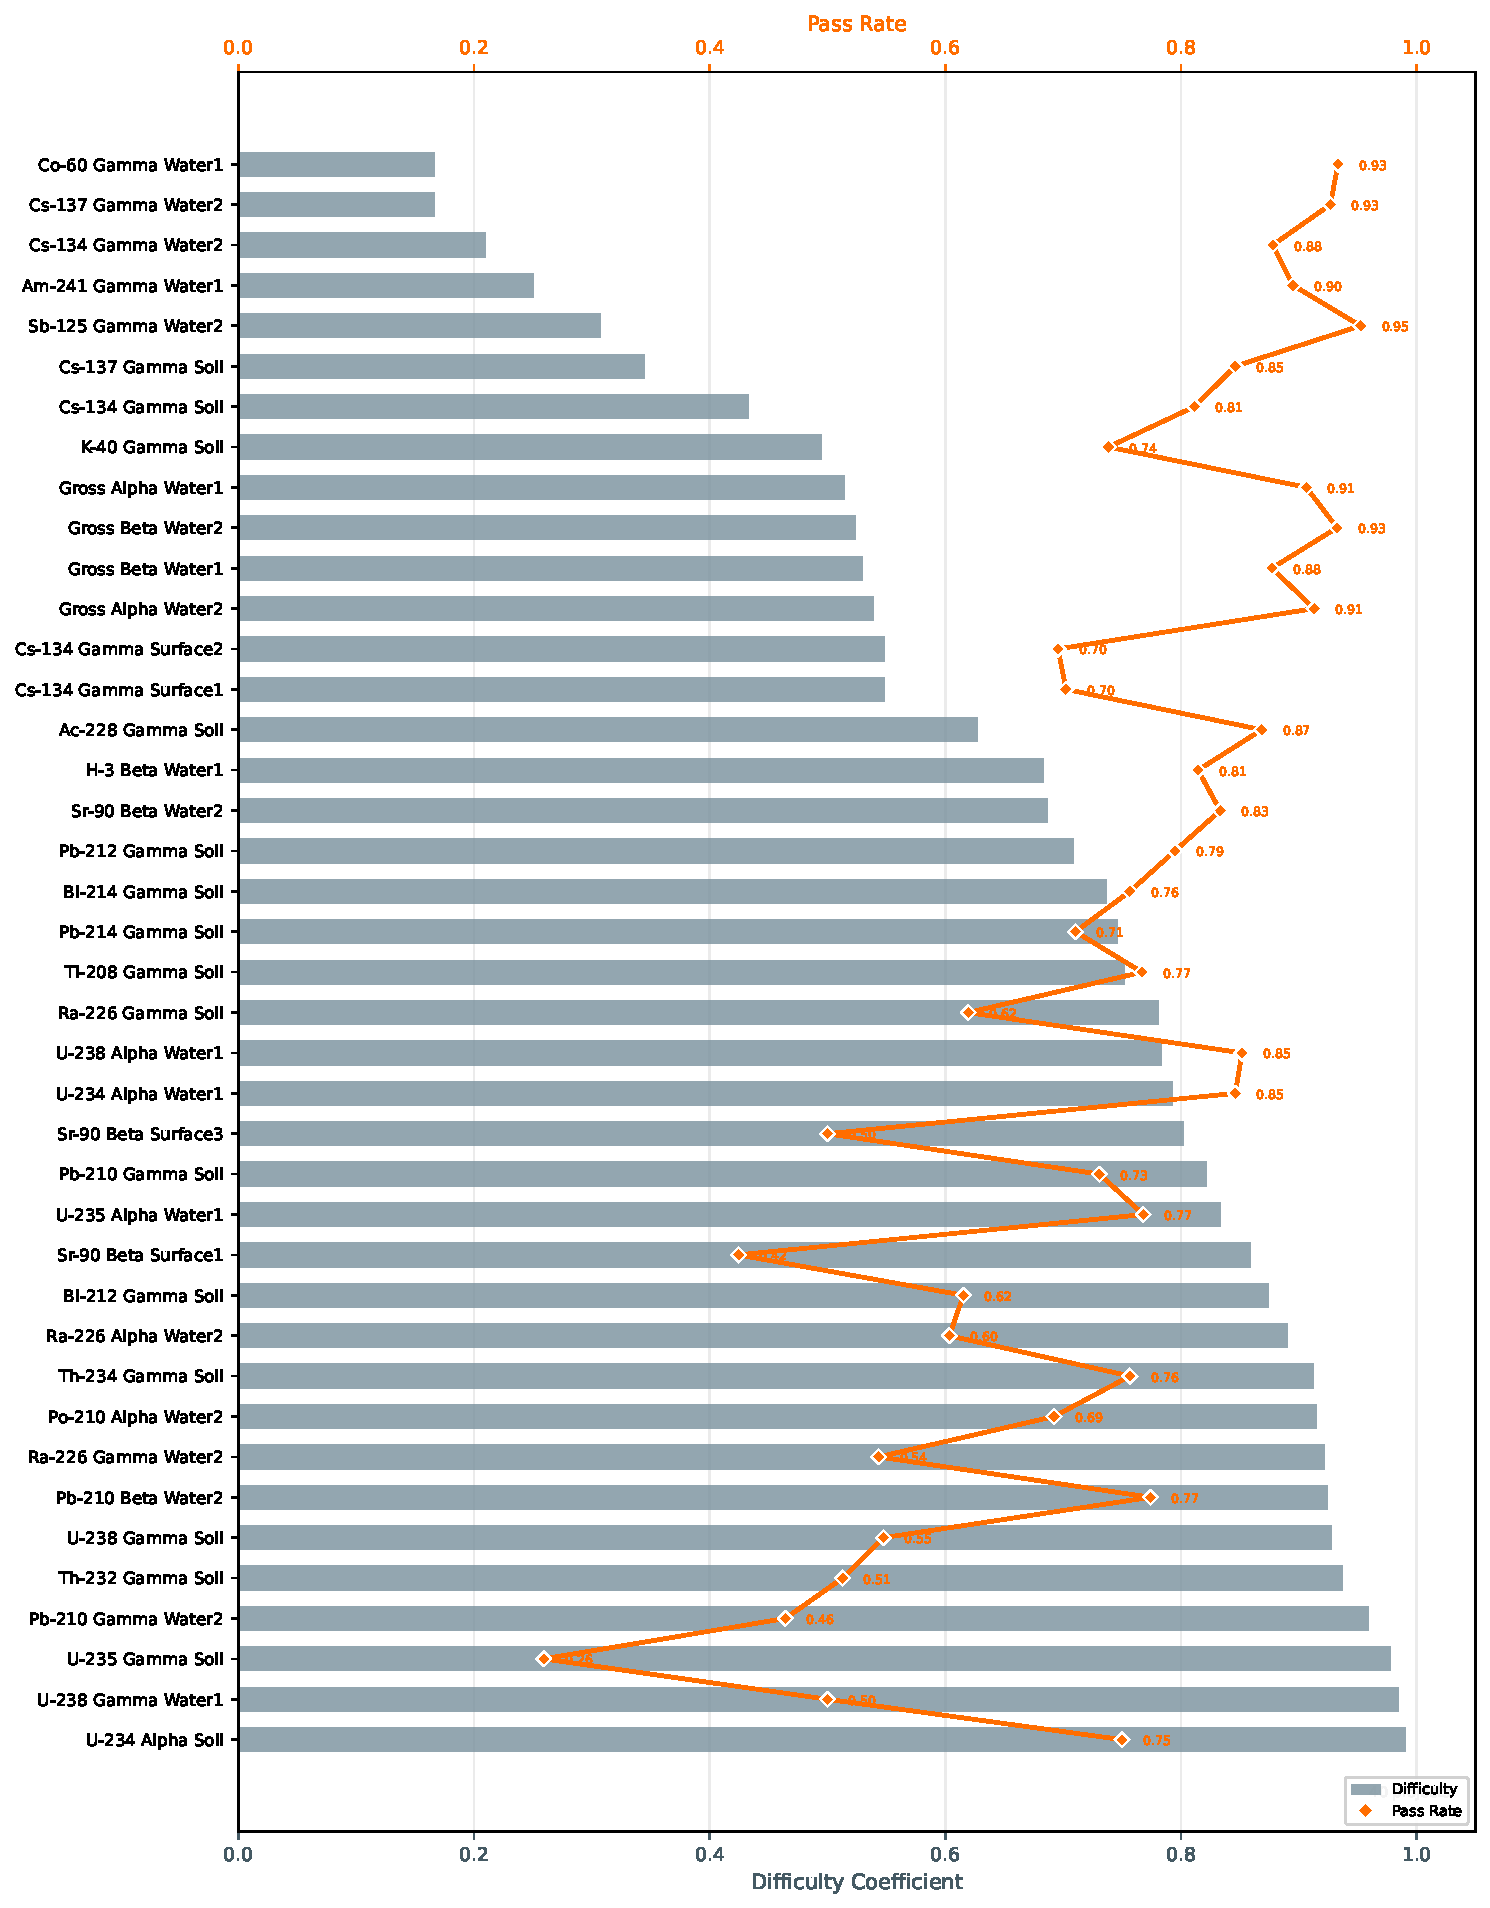
\includegraphics[width=\textwidth,height=6cm,keepaspectratio]{../paper/figures/fig_difficulty_pass_rate_2023.pdf}\\[2pt]{\small 2023: 40项目, $\bar{D}{=}0.685$}
    \end{column}
    \begin{column}{0.48\textwidth}
      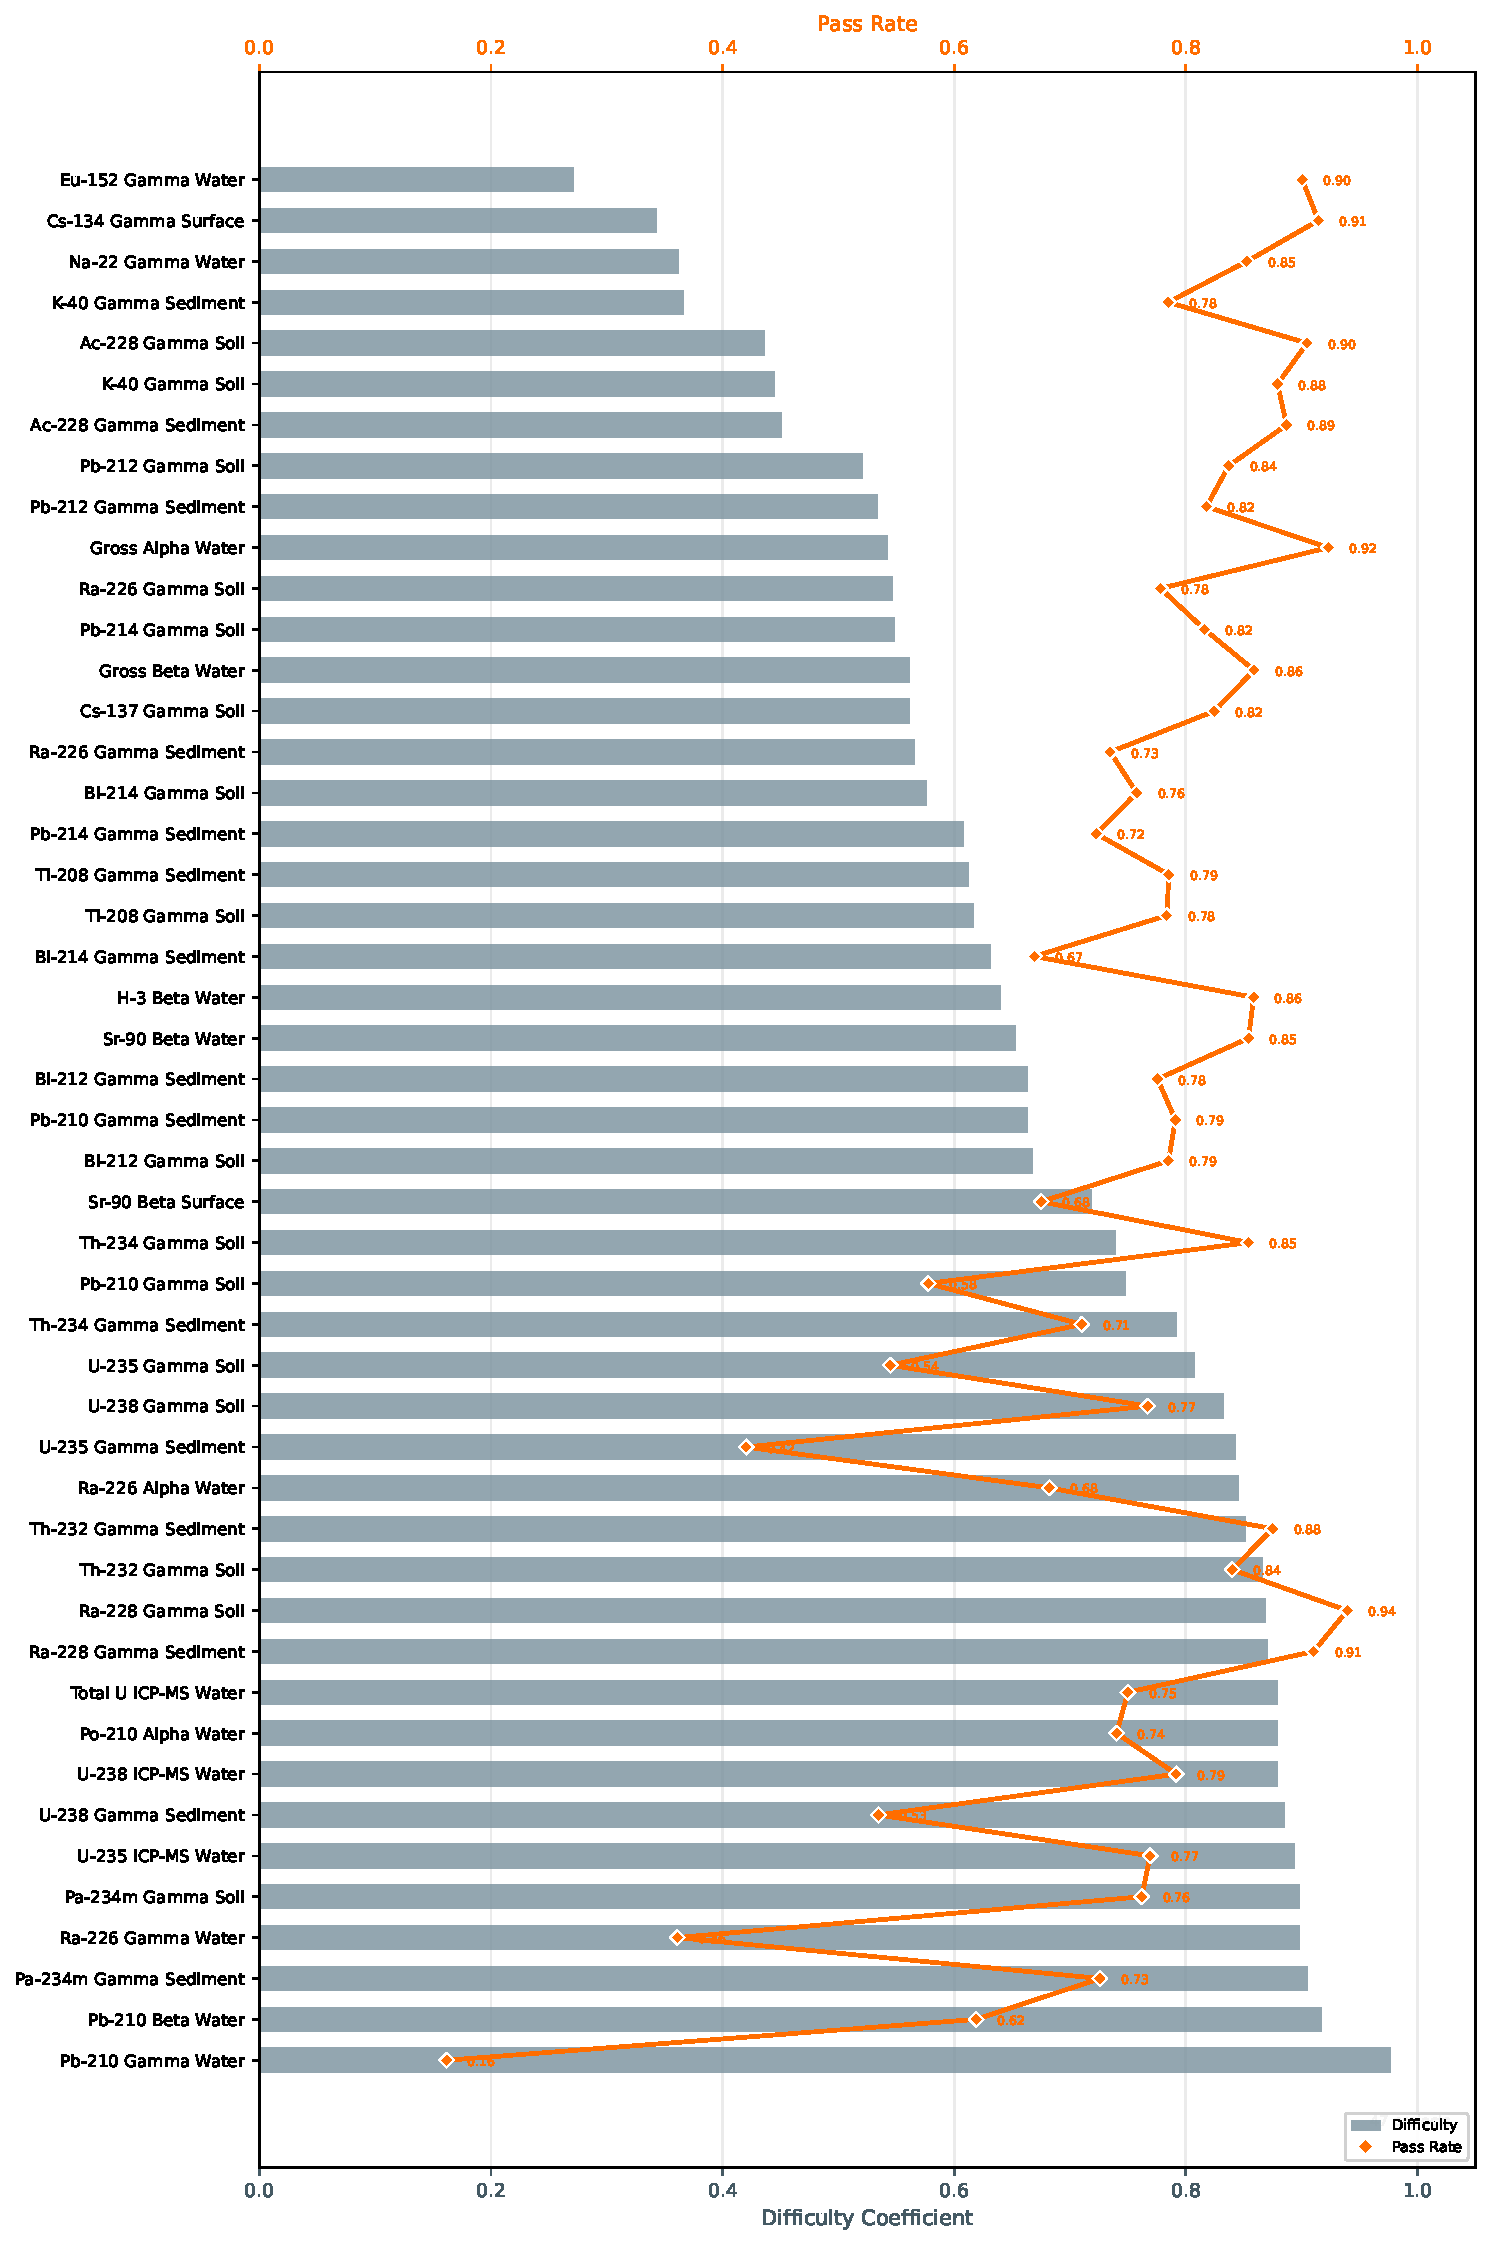
\includegraphics[width=\textwidth,height=6cm,keepaspectratio]{../paper/figures/fig_difficulty_pass_rate_2024.pdf}\\[2pt]{\small 2024: 47项目, $\bar{D}{=}0.685$}
    \end{column}
  \end{columns}
\end{frame}
}

% --- Backup 2: RDI scatter 2021-2024 ---
{
\begin{frame}[plain]{备用：各年度 RDI 散点图 (2021--2024)}
  \centering
  \begin{columns}
    \begin{column}{0.48\textwidth}
      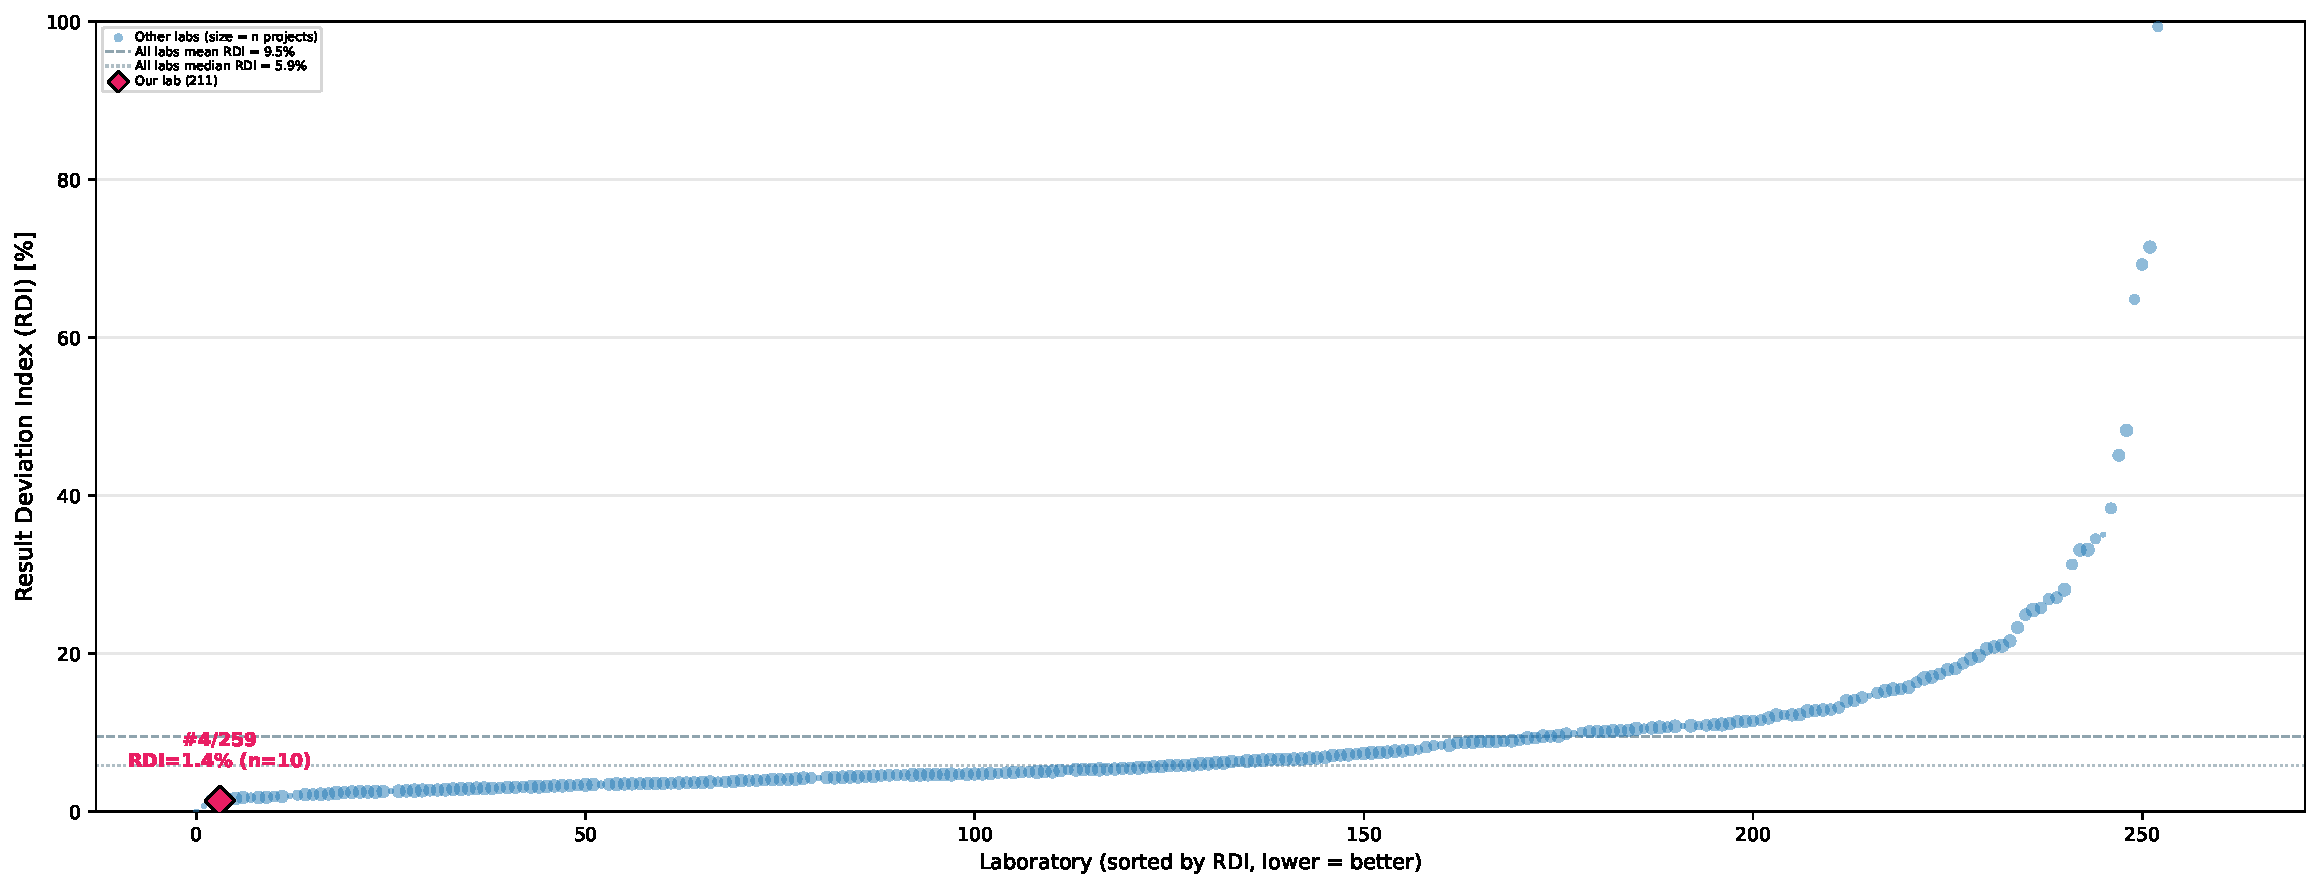
\includegraphics[width=\textwidth,height=5.5cm,keepaspectratio]{../paper/figures/fig_rdi_scatter_2021.pdf}\\[2pt]{\tiny 2021: RDI=1.41\%, \#4/259}
    \end{column}
    \begin{column}{0.48\textwidth}
      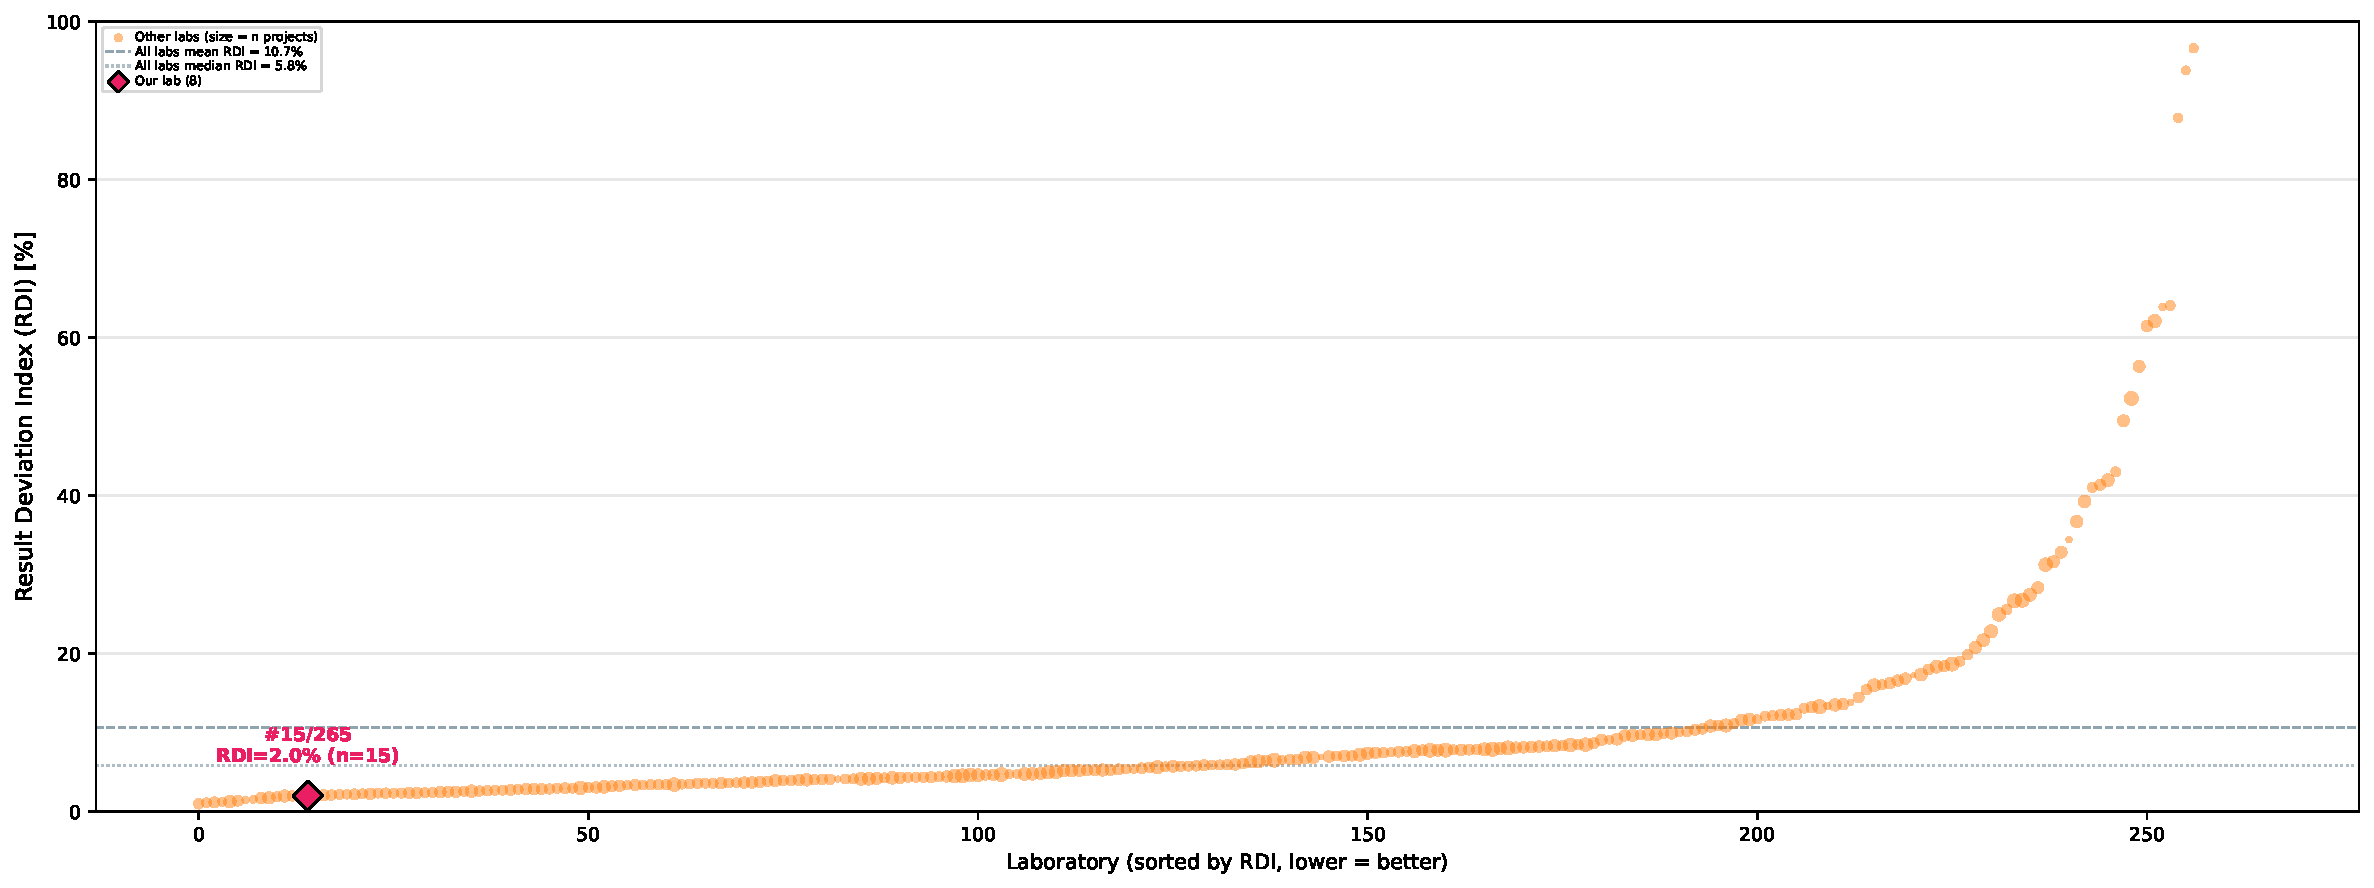
\includegraphics[width=\textwidth,height=5.5cm,keepaspectratio]{../paper/figures/fig_rdi_scatter_2022.pdf}\\[2pt]{\tiny 2022: RDI=2.03\%, \#15/265}
    \end{column}
  \end{columns}
  \vspace{0.1cm}
  \begin{columns}
    \begin{column}{0.48\textwidth}
      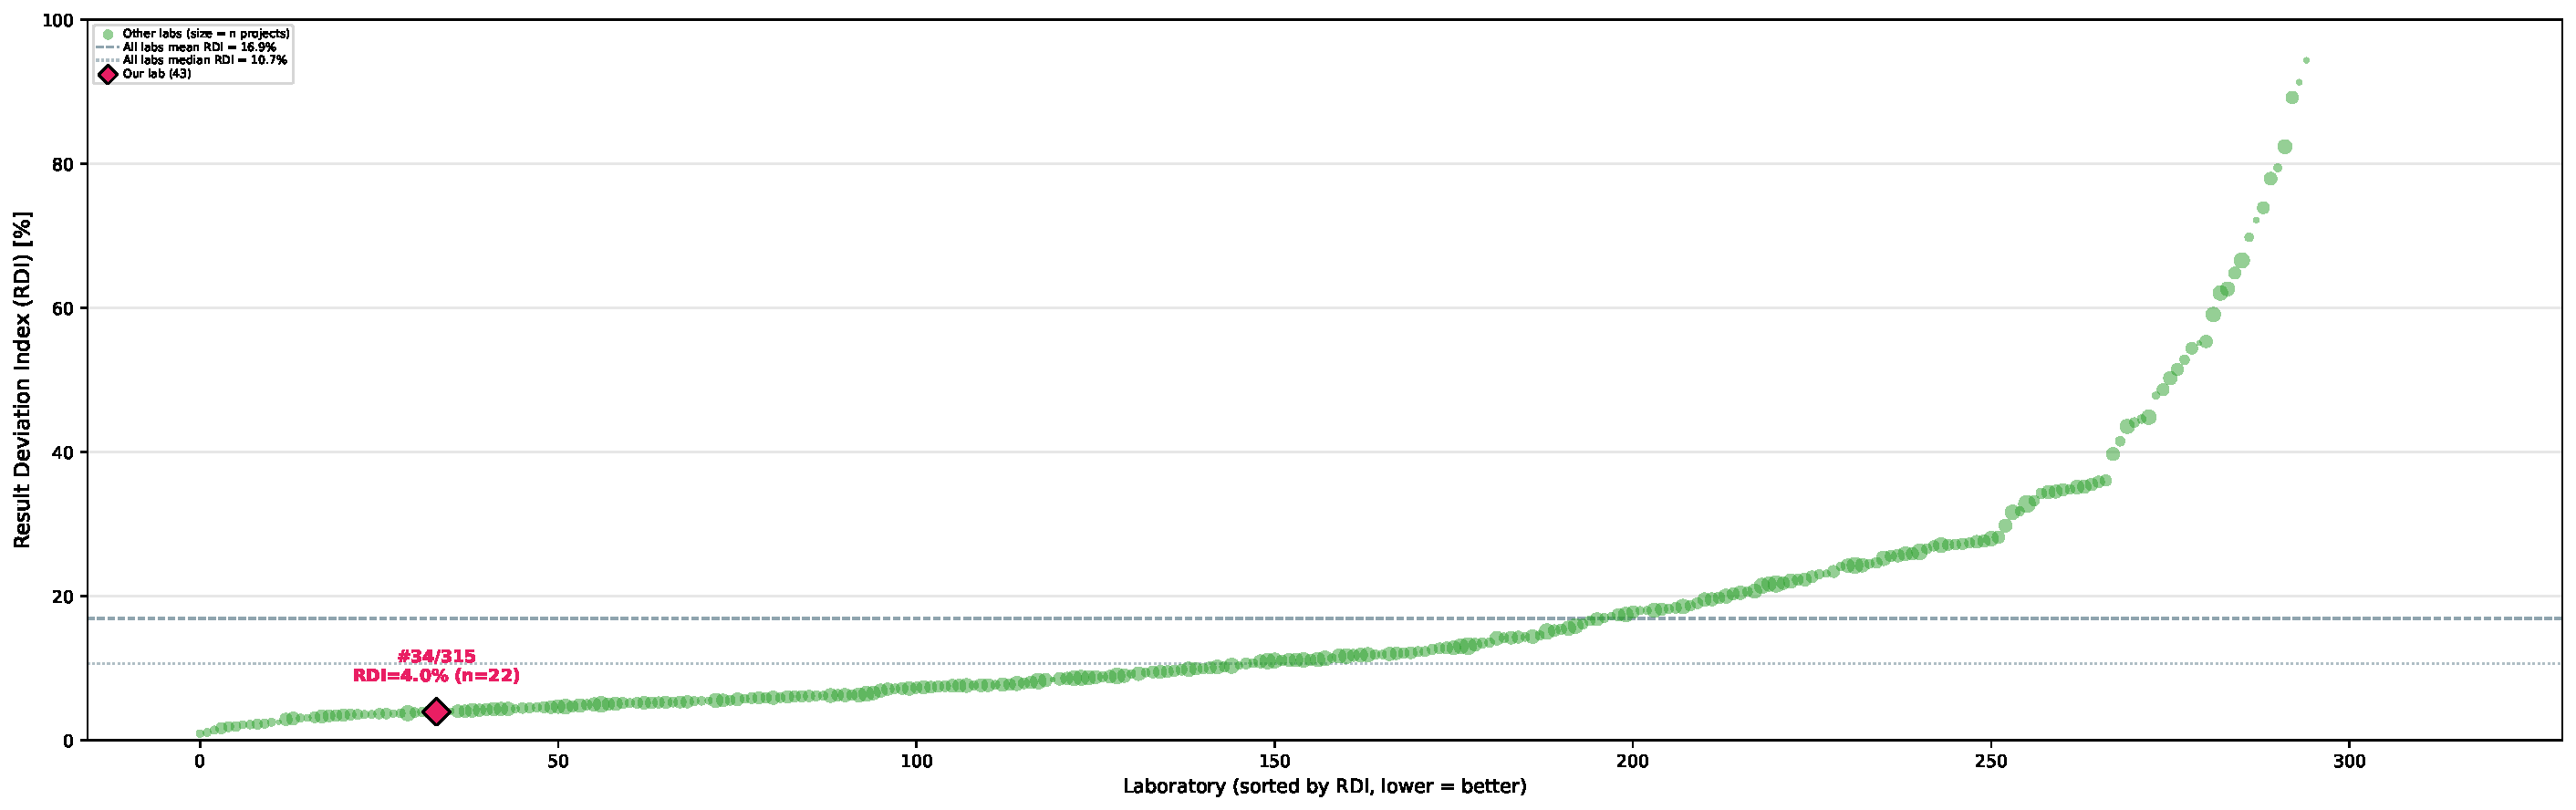
\includegraphics[width=\textwidth,height=5.5cm,keepaspectratio]{../paper/figures/fig_rdi_scatter_2023.pdf}\\[2pt]{\tiny 2023: RDI=3.97\%, \#34/315}
    \end{column}
    \begin{column}{0.48\textwidth}
      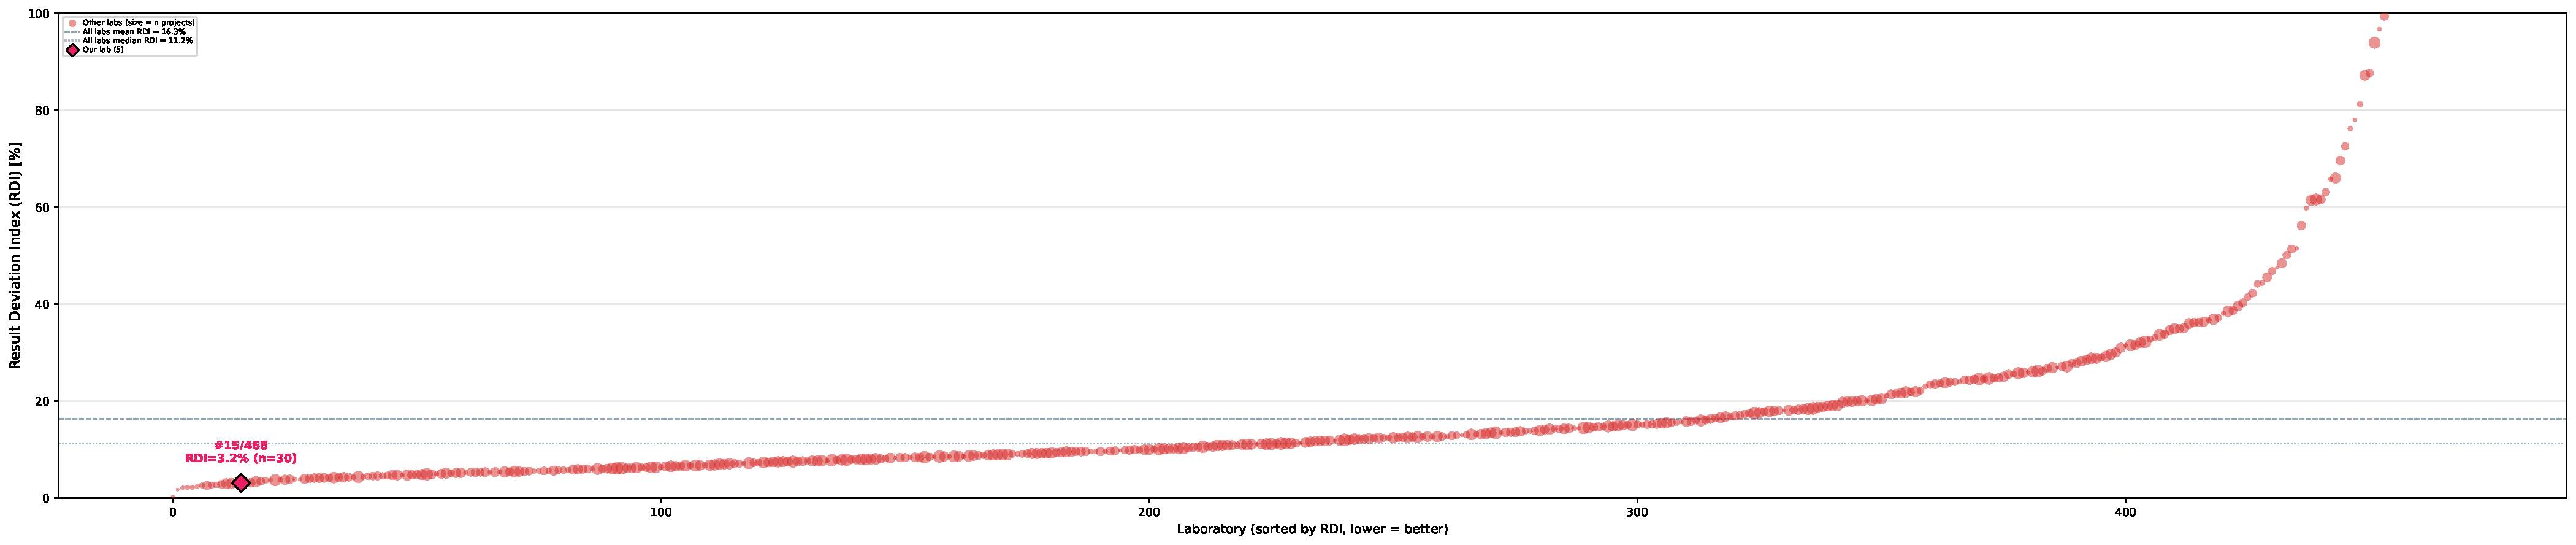
\includegraphics[width=\textwidth,height=5.5cm,keepaspectratio]{../paper/figures/fig_rdi_scatter_2024.pdf}\\[2pt]{\tiny 2024: RDI=3.16\%, \#15/468}
    \end{column}
  \end{columns}
\end{frame}
}

% --- Backup 3a: Ranking 2021-2022 ---
{
\begin{frame}[plain]{备用：各年度百分位排名 (2021--2022)}
  \centering
  \begin{columns}
    \begin{column}{0.48\textwidth}
      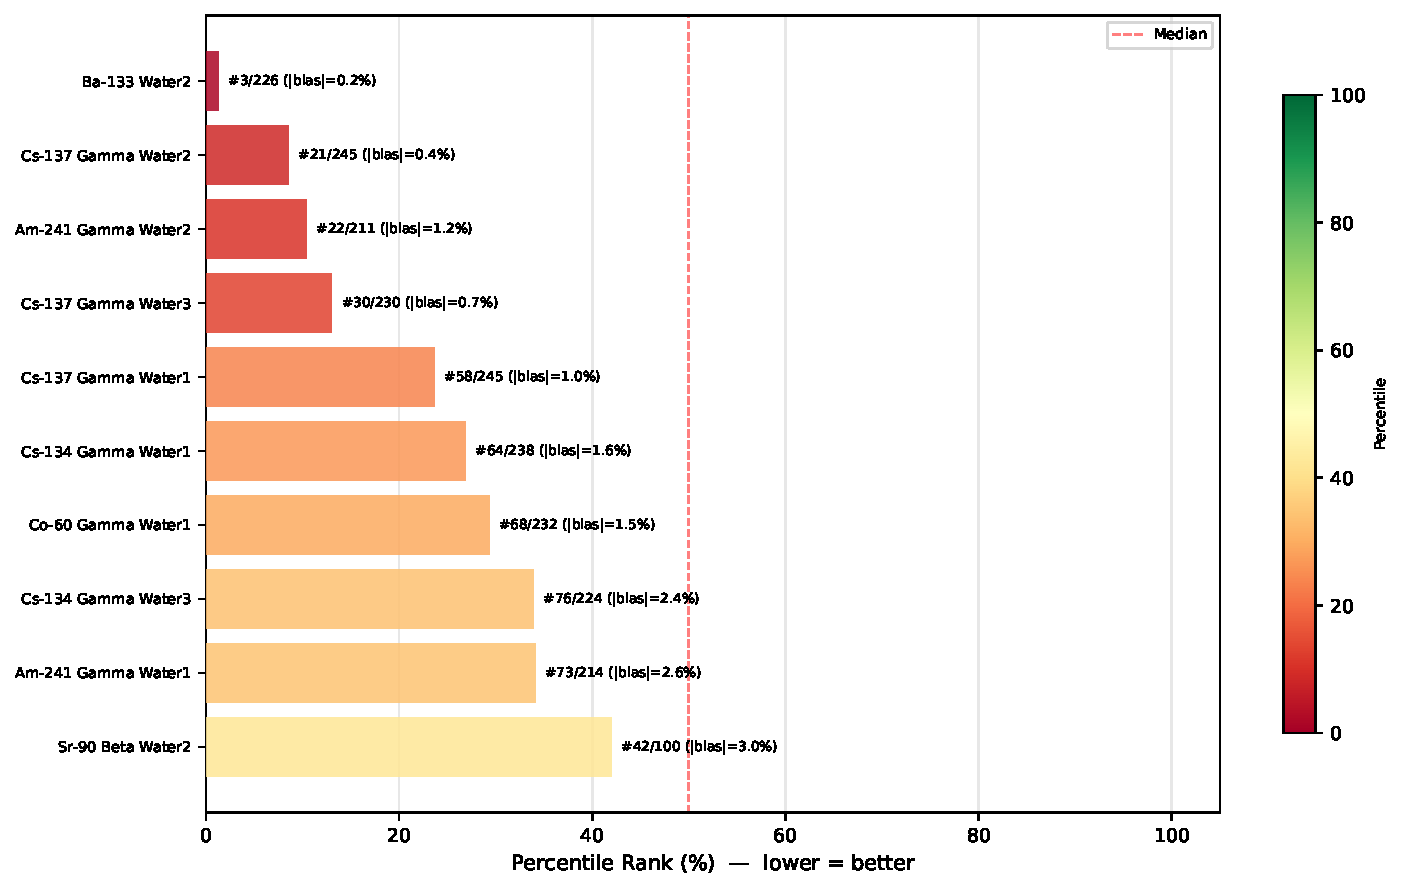
\includegraphics[width=\textwidth,height=7cm,keepaspectratio]{../paper/figures/fig_ranking_2021.pdf}\\[2pt]{\small 2021: 均值22.3\%, 中位25.3\%}
    \end{column}
    \begin{column}{0.48\textwidth}
      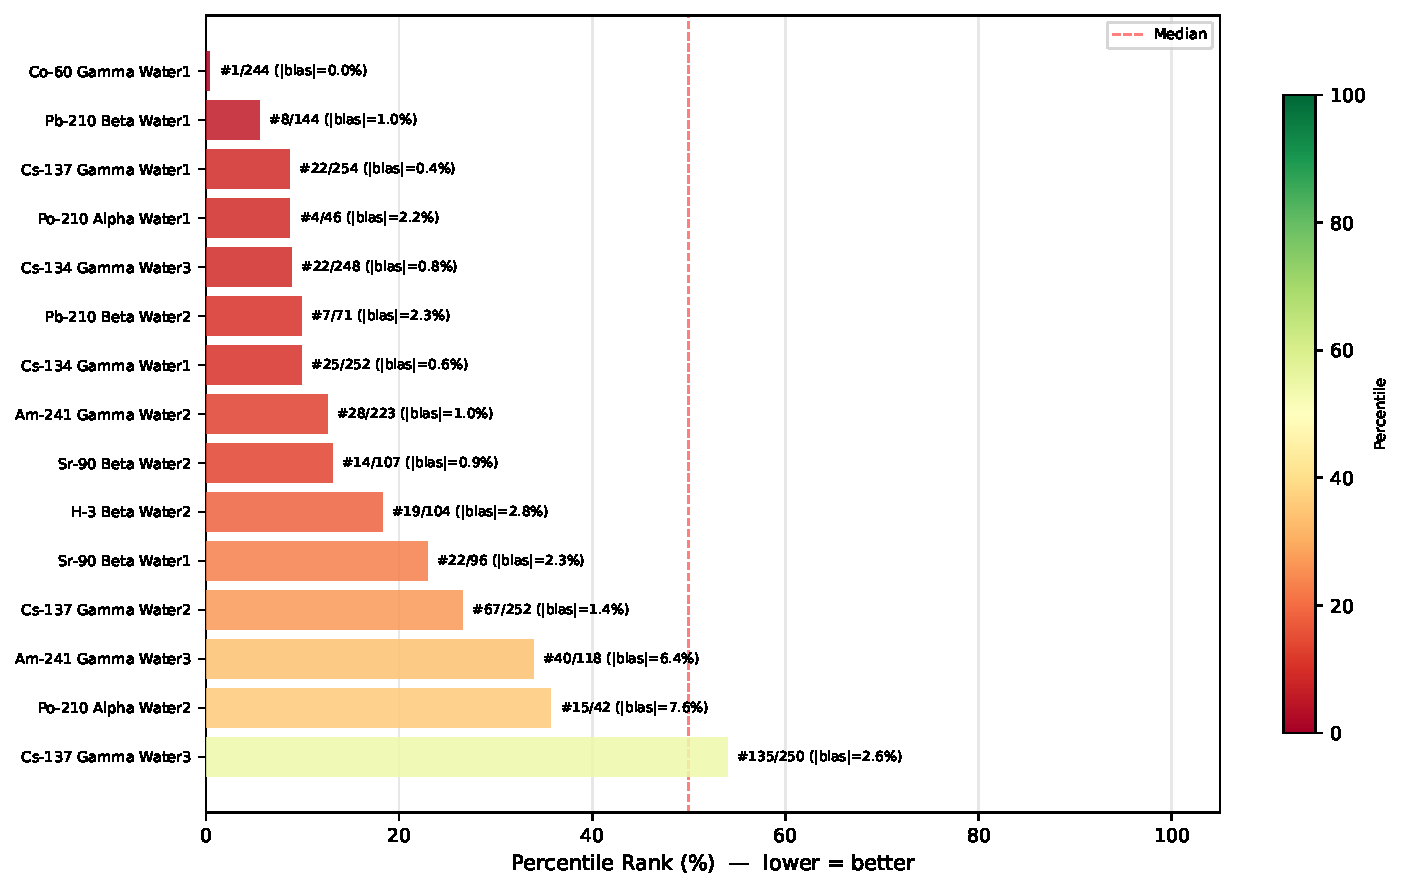
\includegraphics[width=\textwidth,height=7cm,keepaspectratio]{../paper/figures/fig_ranking_2022.pdf}\\[2pt]{\small 2022: 均值17.9\%, 中位12.6\%}
    \end{column}
  \end{columns}
\end{frame}
}

% --- Backup 3b: Ranking 2023-2024 ---
{
\begin{frame}[plain]{备用：各年度百分位排名 (2023--2024)}
  \centering
  \begin{columns}
    \begin{column}{0.48\textwidth}
      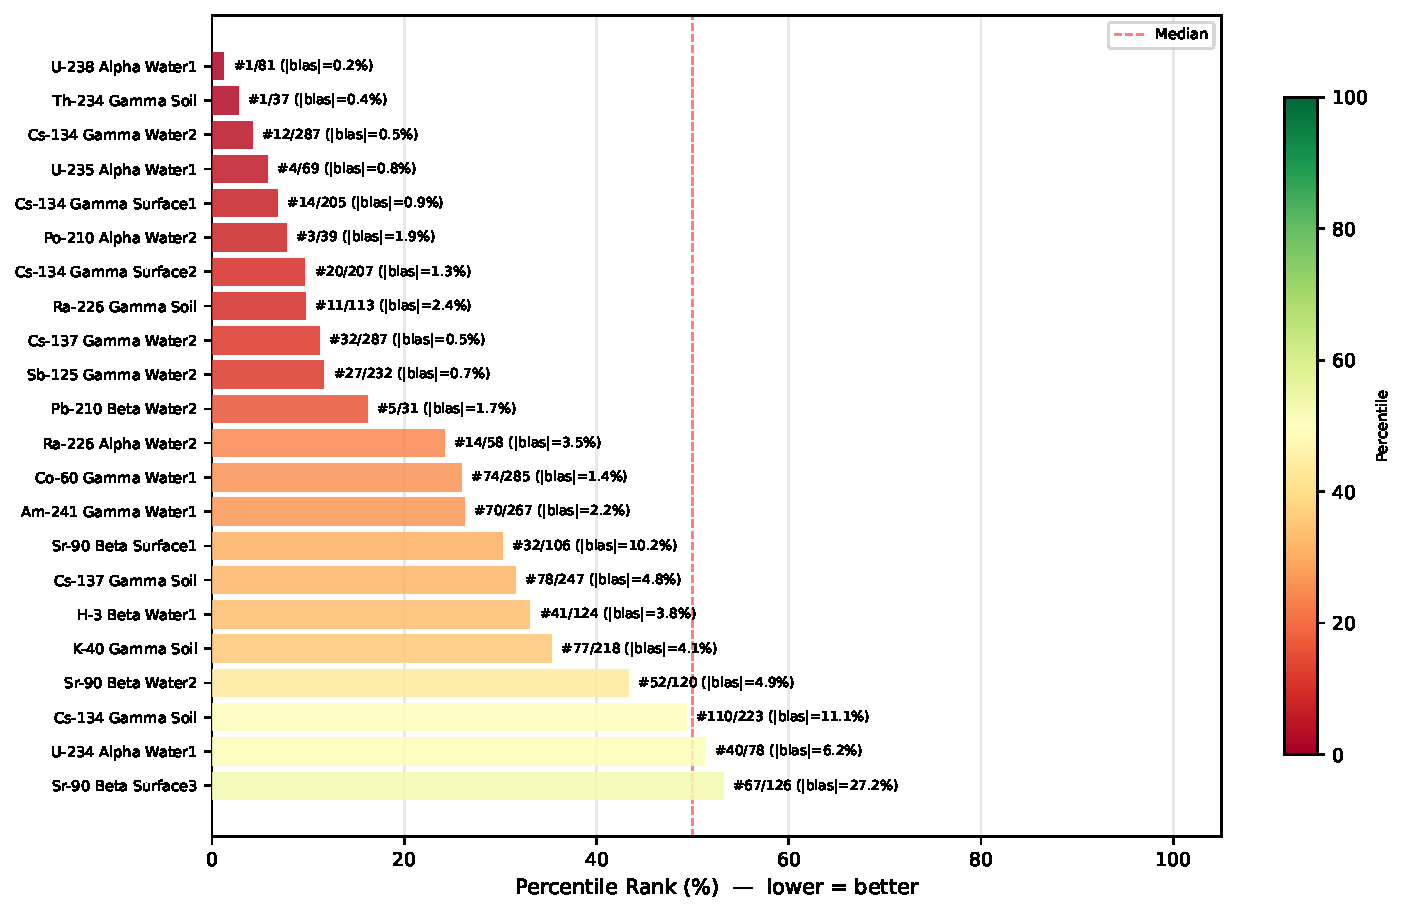
\includegraphics[width=\textwidth,height=7cm,keepaspectratio]{../paper/figures/fig_ranking_2023.pdf}\\[2pt]{\small 2023: 均值22.3\%, 中位20.1\%}
    \end{column}
    \begin{column}{0.48\textwidth}
      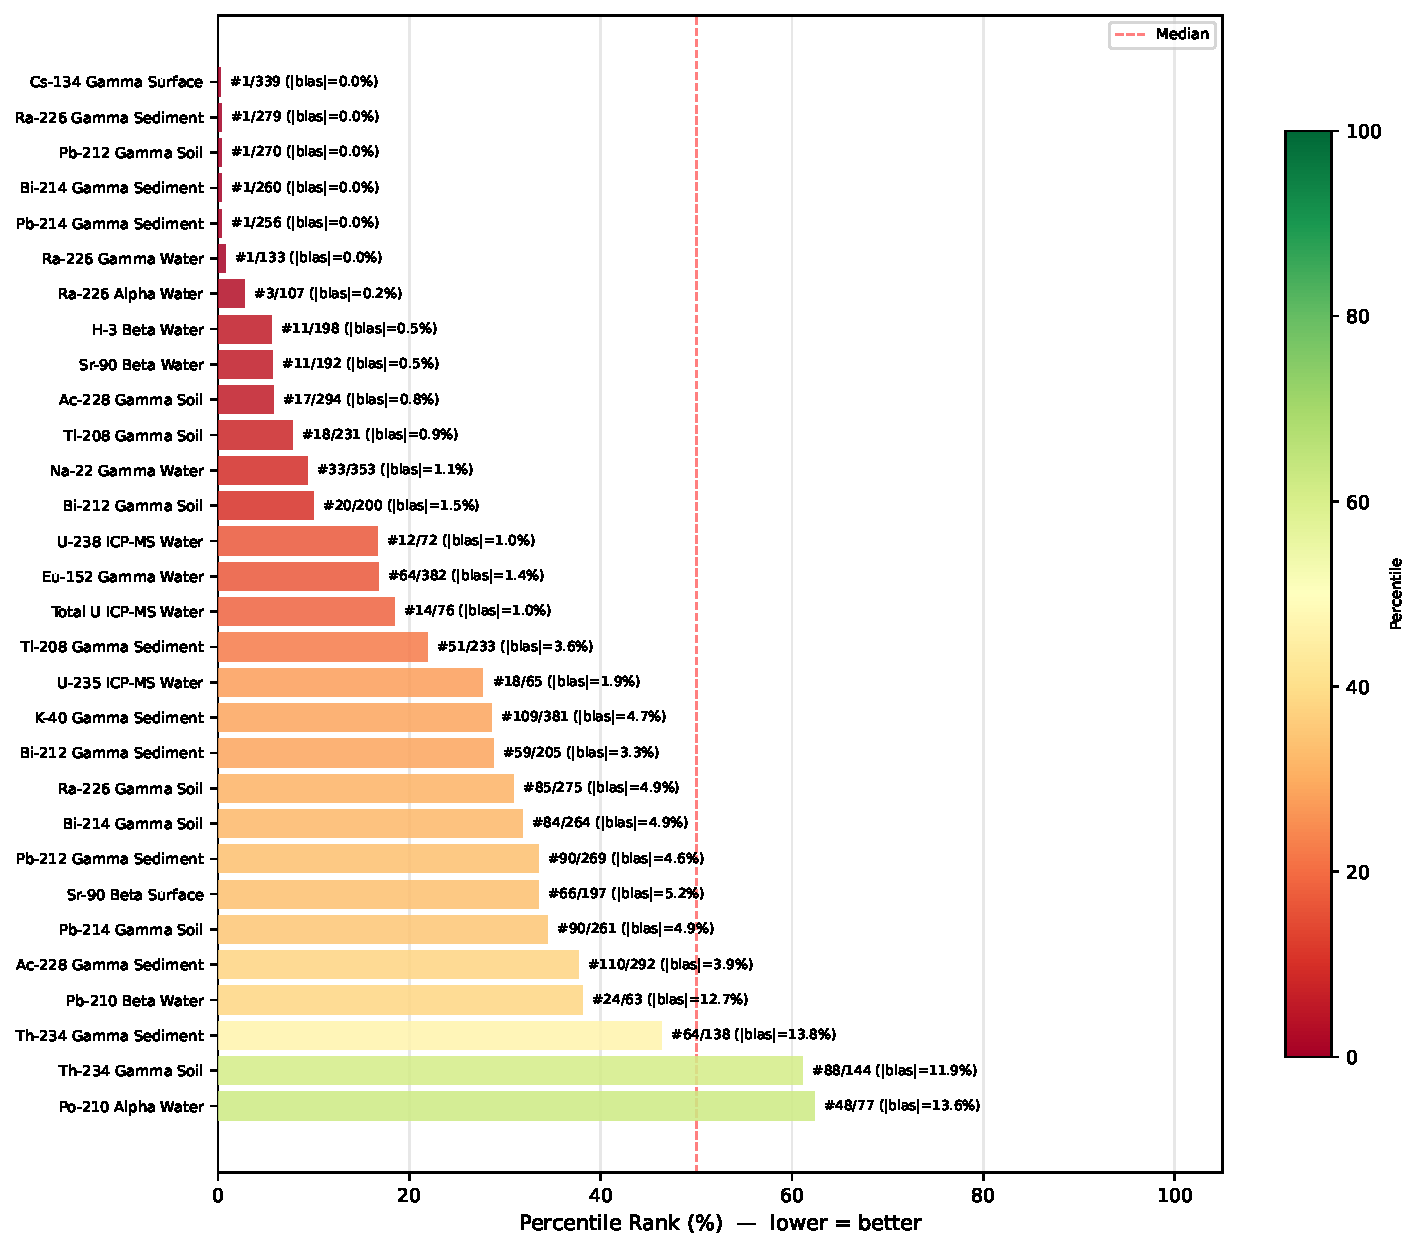
\includegraphics[width=\textwidth,height=7cm,keepaspectratio]{../paper/figures/fig_ranking_2024.pdf}\\[2pt]{\small 2024: 均值20.6\%, 中位17.6\%}
    \end{column}
  \end{columns}
\end{frame}
}

% --- Backup 4a: Bias 2021-2022 ---
{
\begin{frame}[plain]{备用：各年度相对偏差分布 (2021--2022)}
  \centering
  \begin{columns}
    \begin{column}{0.48\textwidth}
      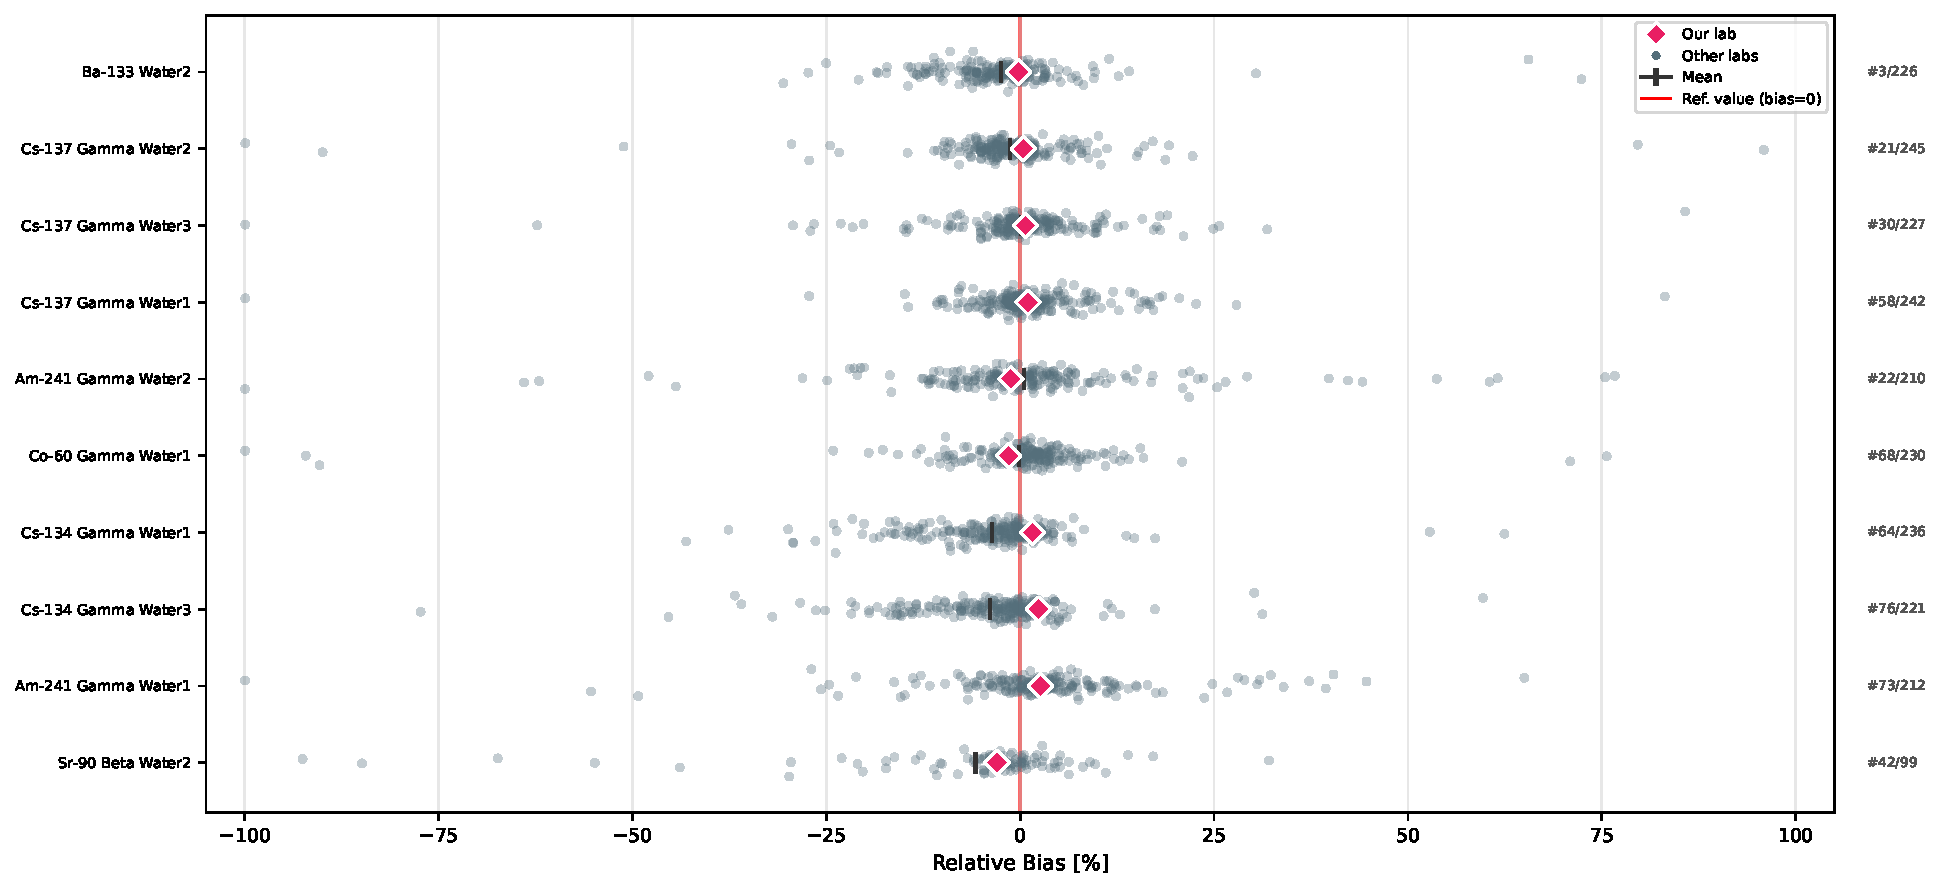
\includegraphics[width=\textwidth,height=7cm,keepaspectratio]{../paper/figures/fig_relative_bias_2021.pdf}\\[2pt]{\small 2021}
    \end{column}
    \begin{column}{0.48\textwidth}
      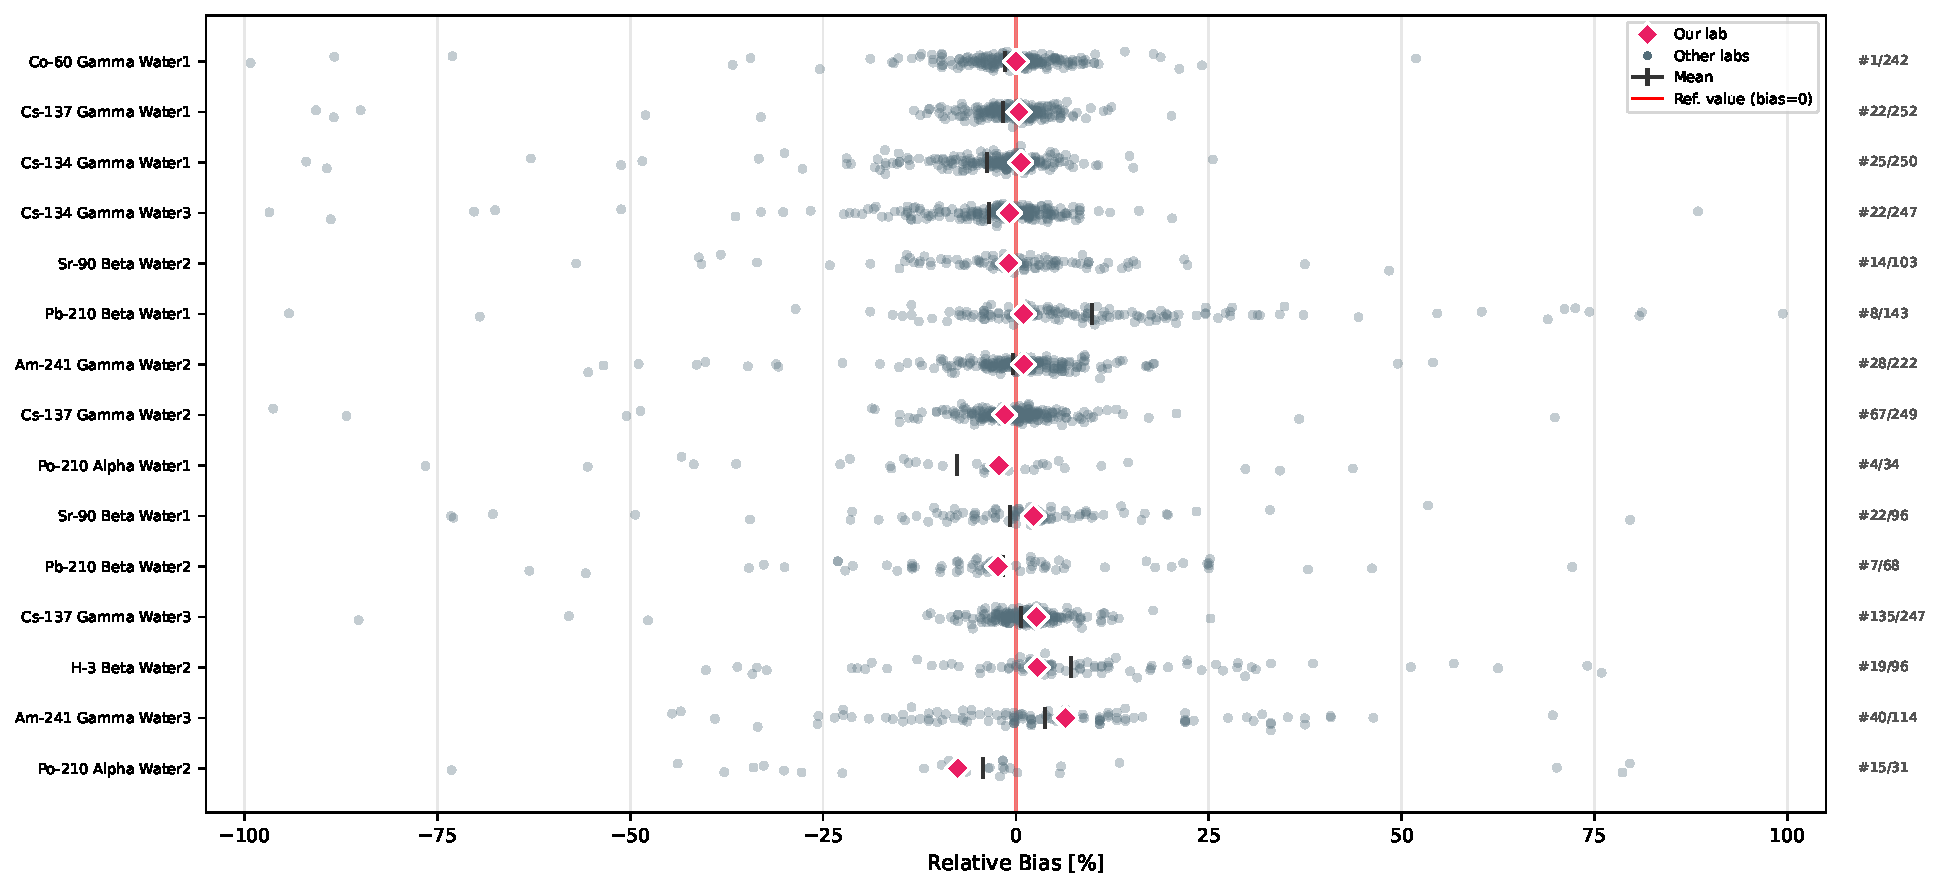
\includegraphics[width=\textwidth,height=7cm,keepaspectratio]{../paper/figures/fig_relative_bias_2022.pdf}\\[2pt]{\small 2022}
    \end{column}
  \end{columns}
\end{frame}
}

% --- Backup 4b: Bias 2023-2024 ---
{
\begin{frame}[plain]{备用：各年度相对偏差分布 (2023--2024)}
  \centering
  \begin{columns}
    \begin{column}{0.48\textwidth}
      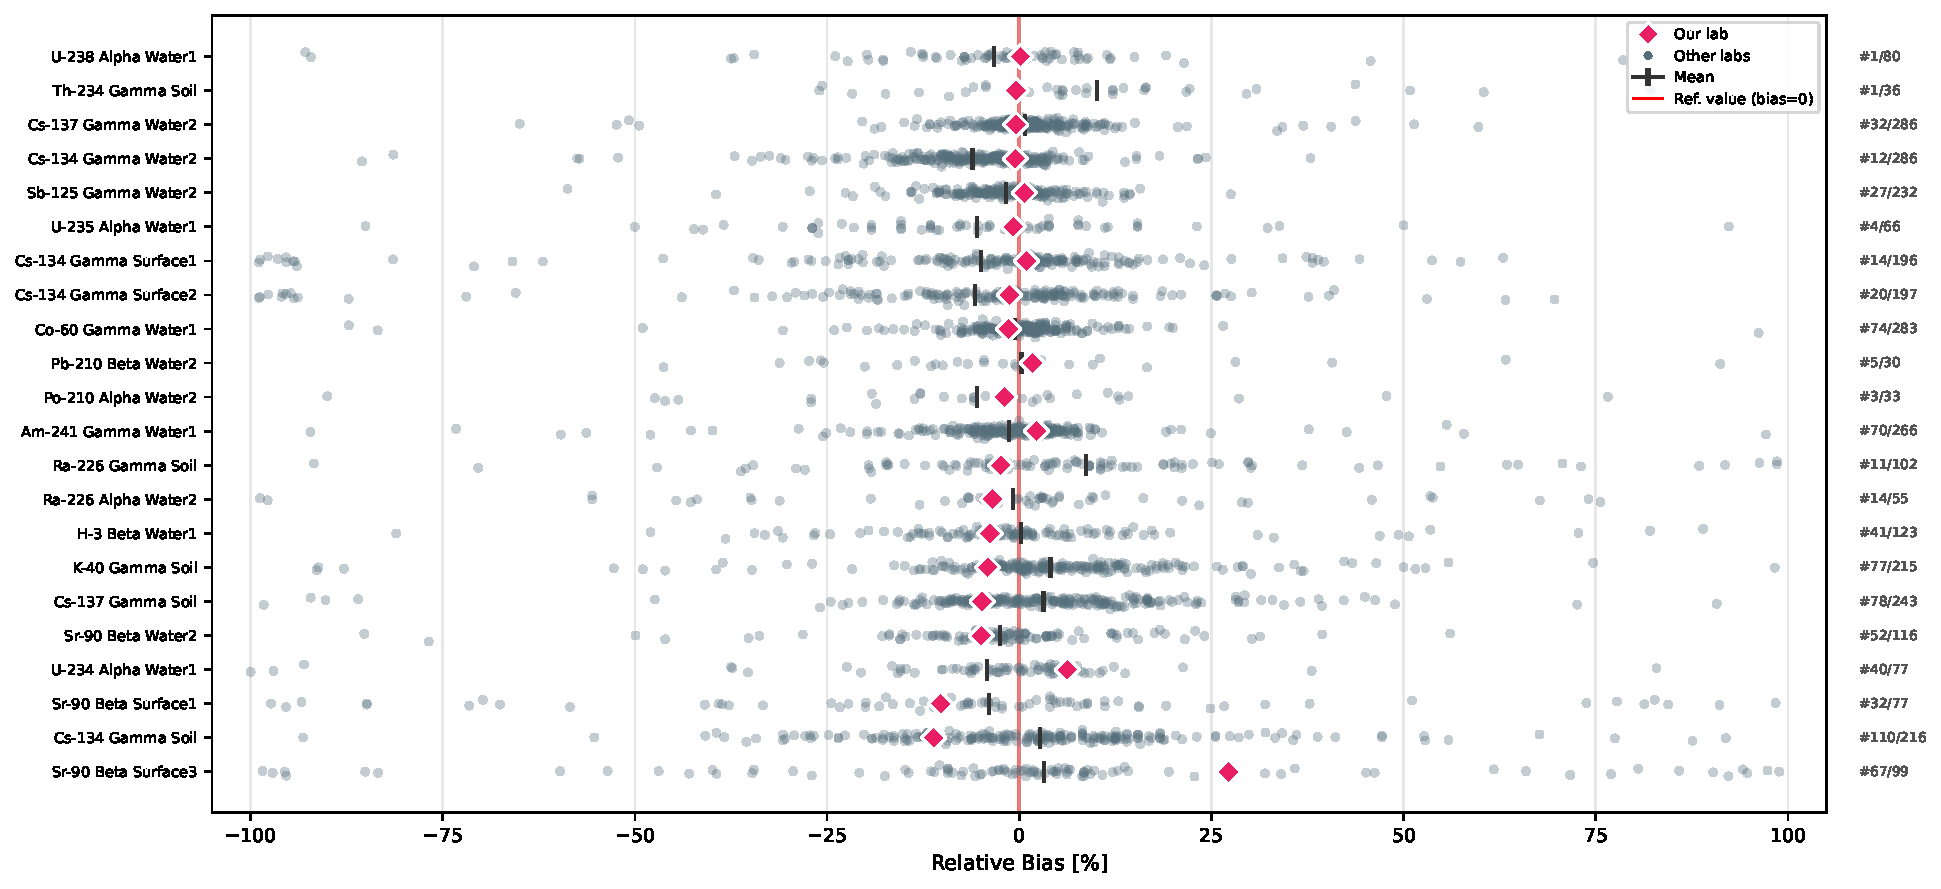
\includegraphics[width=\textwidth,height=7cm,keepaspectratio]{../paper/figures/fig_relative_bias_2023.pdf}\\[2pt]{\small 2023}
    \end{column}
    \begin{column}{0.48\textwidth}
      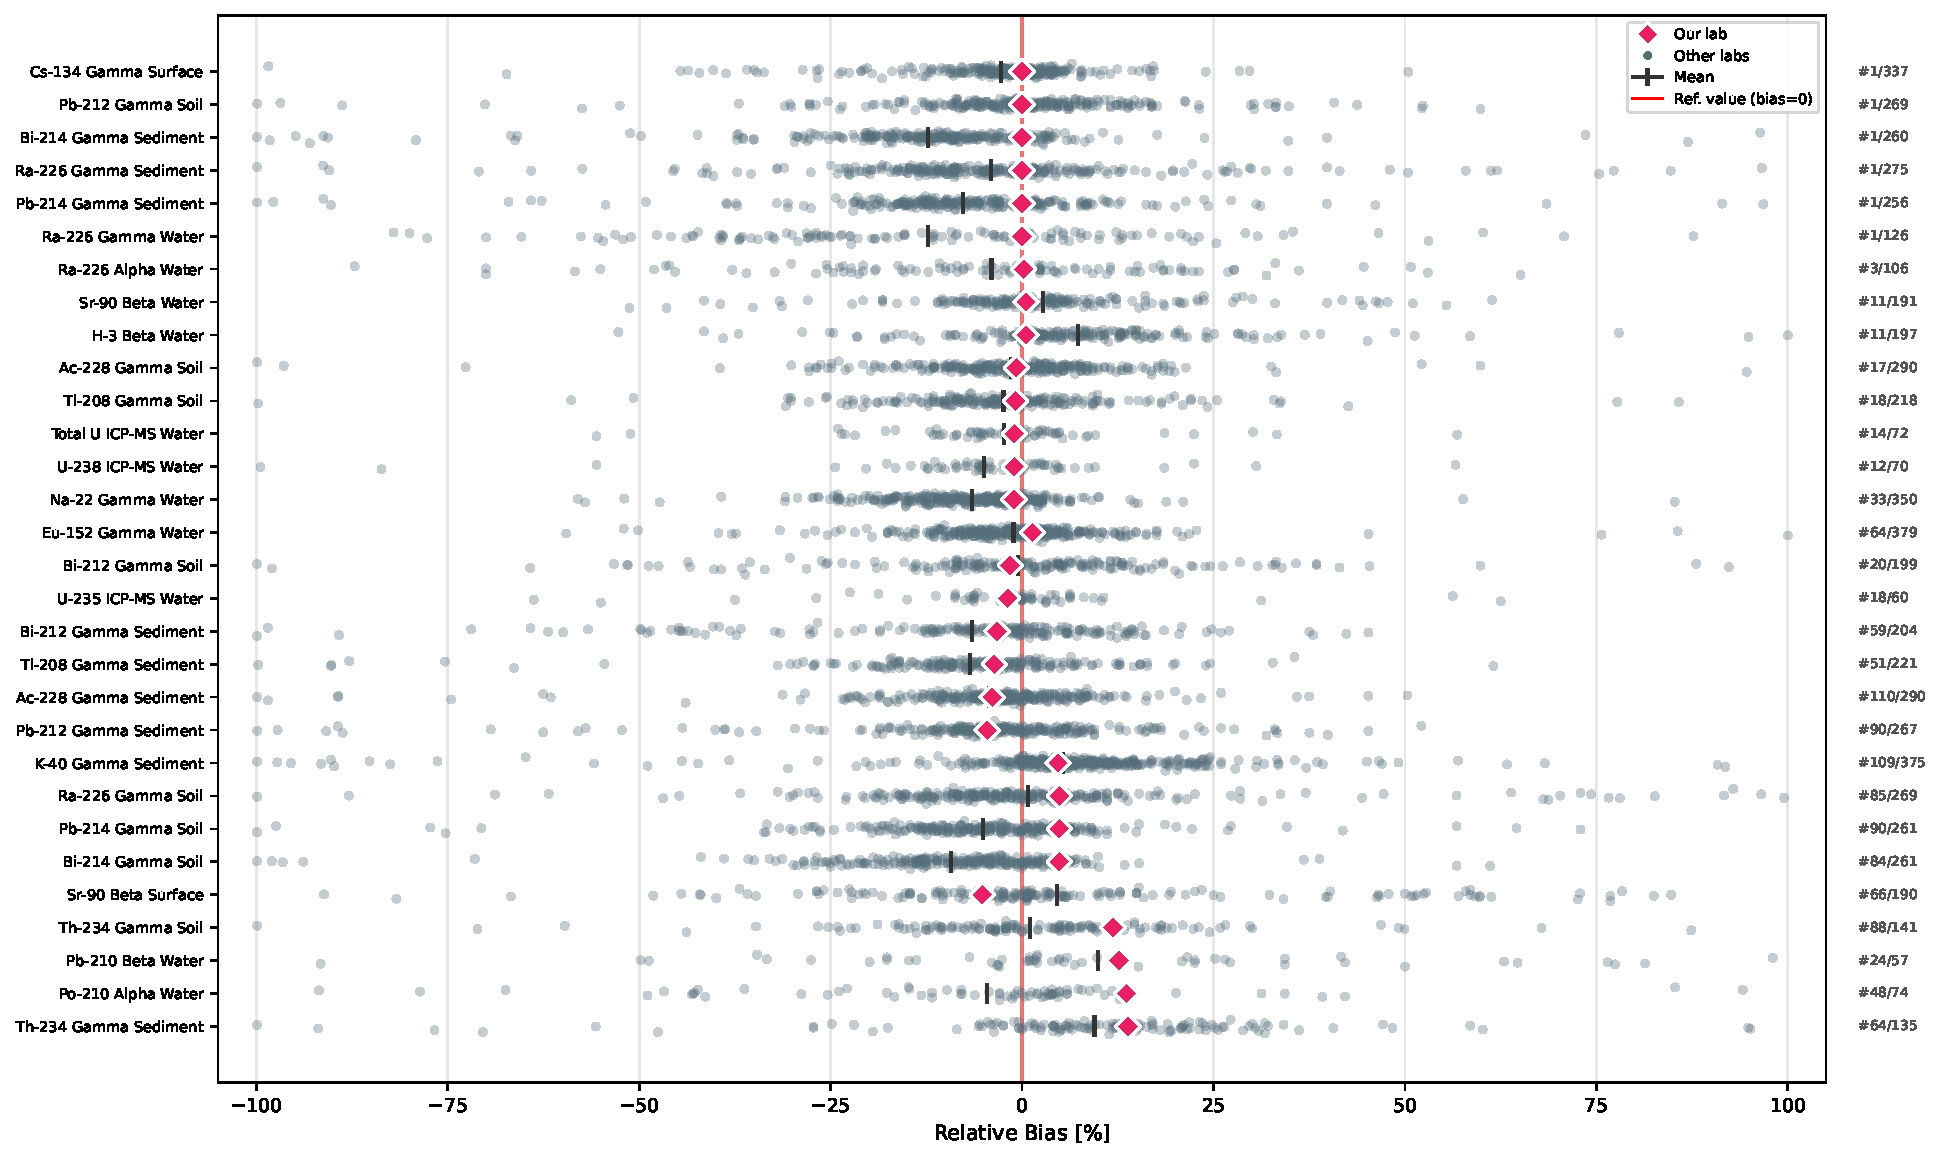
\includegraphics[width=\textwidth,height=7cm,keepaspectratio]{../paper/figures/fig_relative_bias_2024.pdf}\\[2pt]{\small 2024}
    \end{column}
  \end{columns}
\end{frame}
}

% --- Backup 5: Lab scatter + RDI ranking ---
{
\begin{frame}[plain]{备用：实验室参与散点图 + RDI 排名}
  \centering
  \begin{columns}
    \begin{column}{0.33\textwidth}
      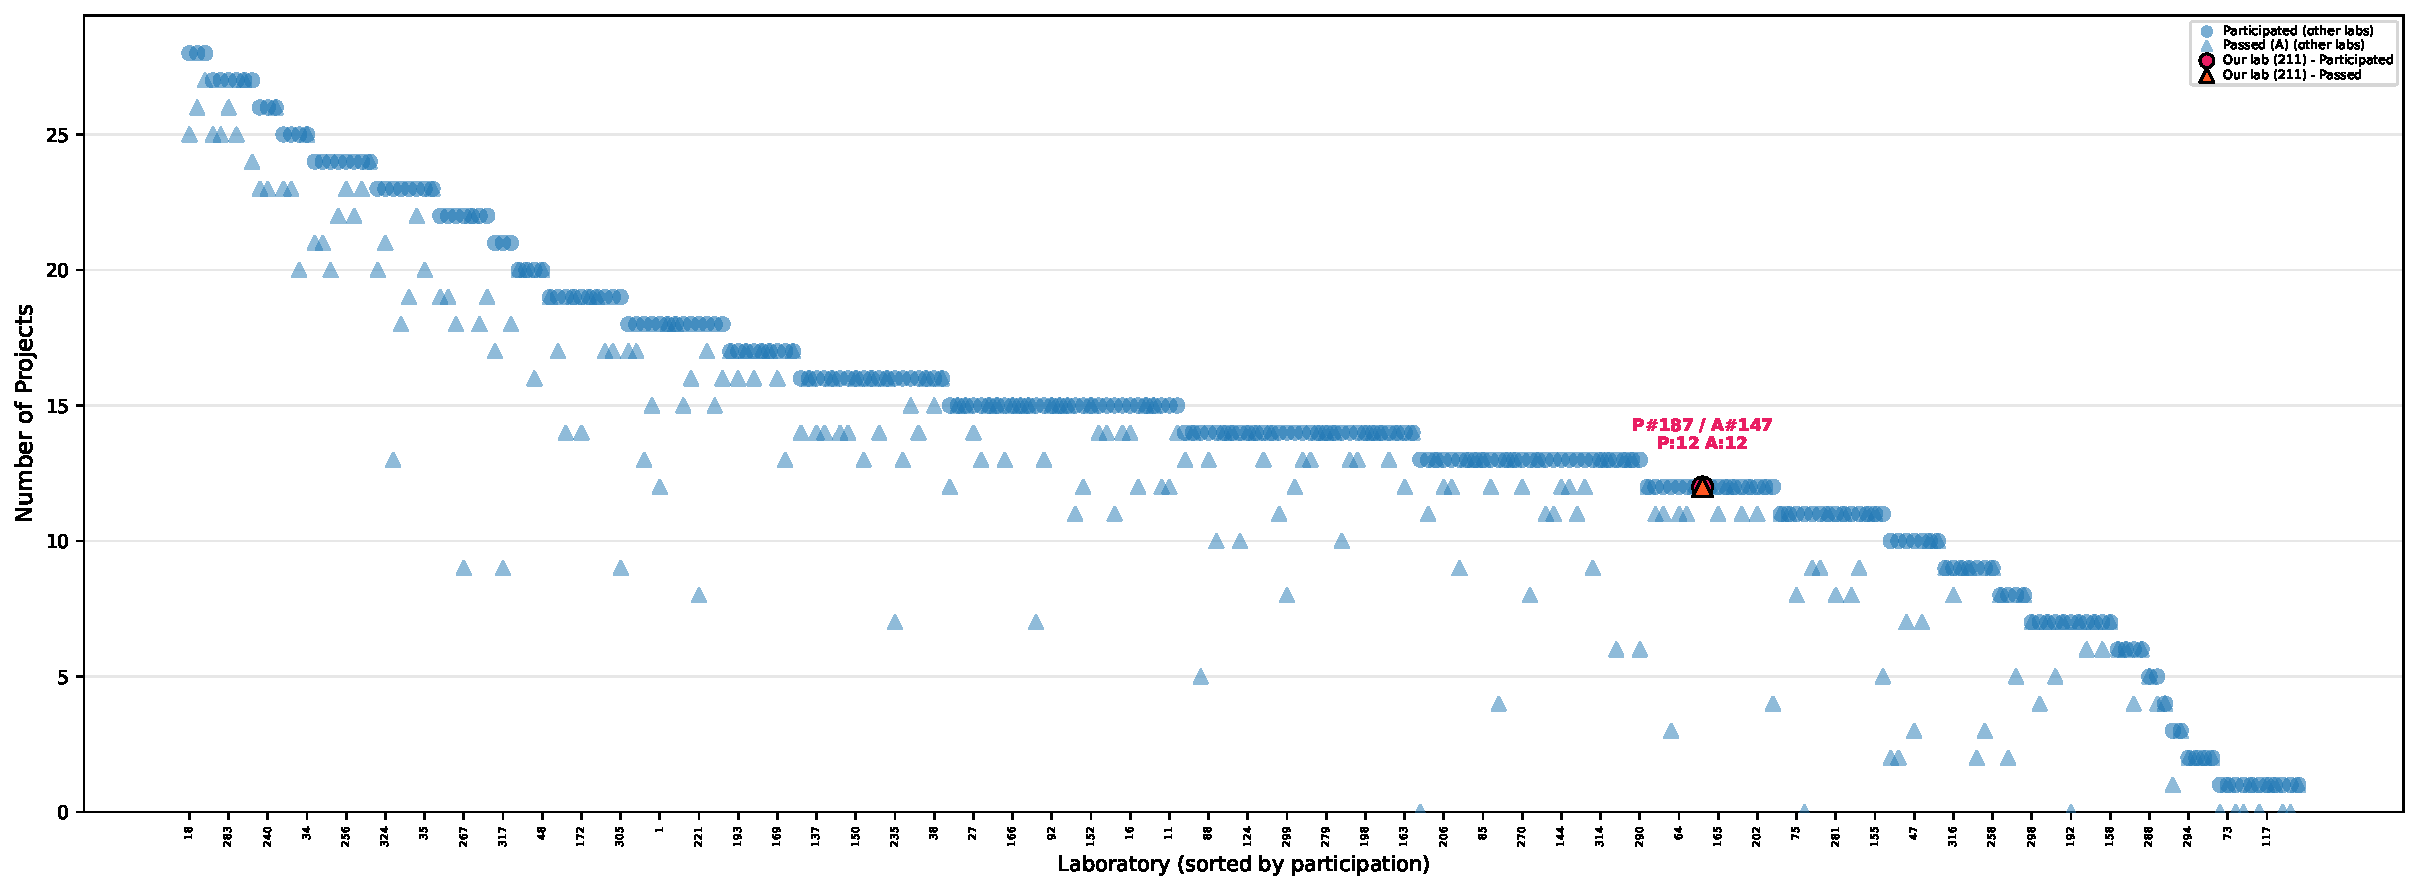
\includegraphics[width=\textwidth,height=4.5cm,keepaspectratio]{../paper/figures/fig_lab_performance_2021.pdf}\\[2pt]{\tiny 2021: P\#187/A\#147}
    \end{column}
    \begin{column}{0.33\textwidth}
      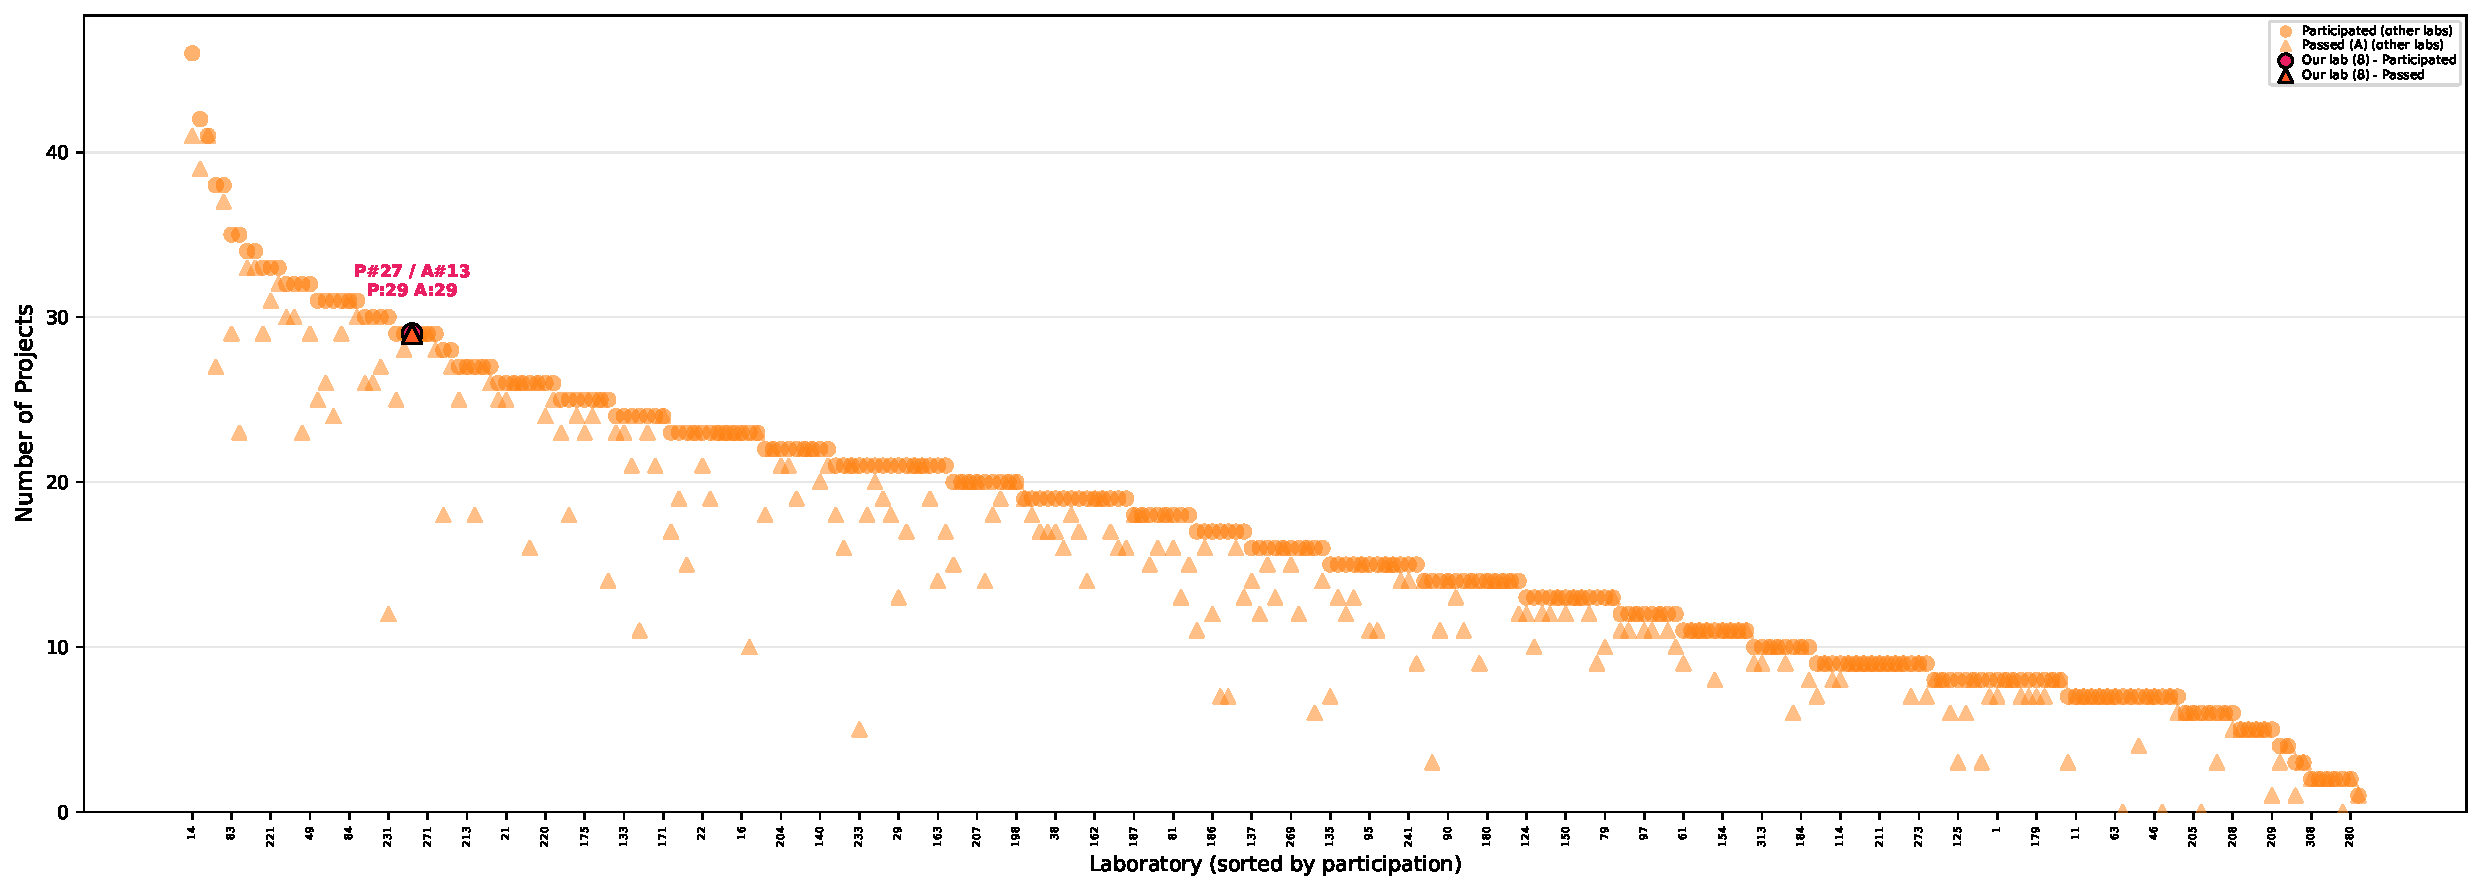
\includegraphics[width=\textwidth,height=4.5cm,keepaspectratio]{../paper/figures/fig_lab_performance_2022.pdf}\\[2pt]{\tiny 2022: P\#27/A\#13}
    \end{column}
    \begin{column}{0.33\textwidth}
      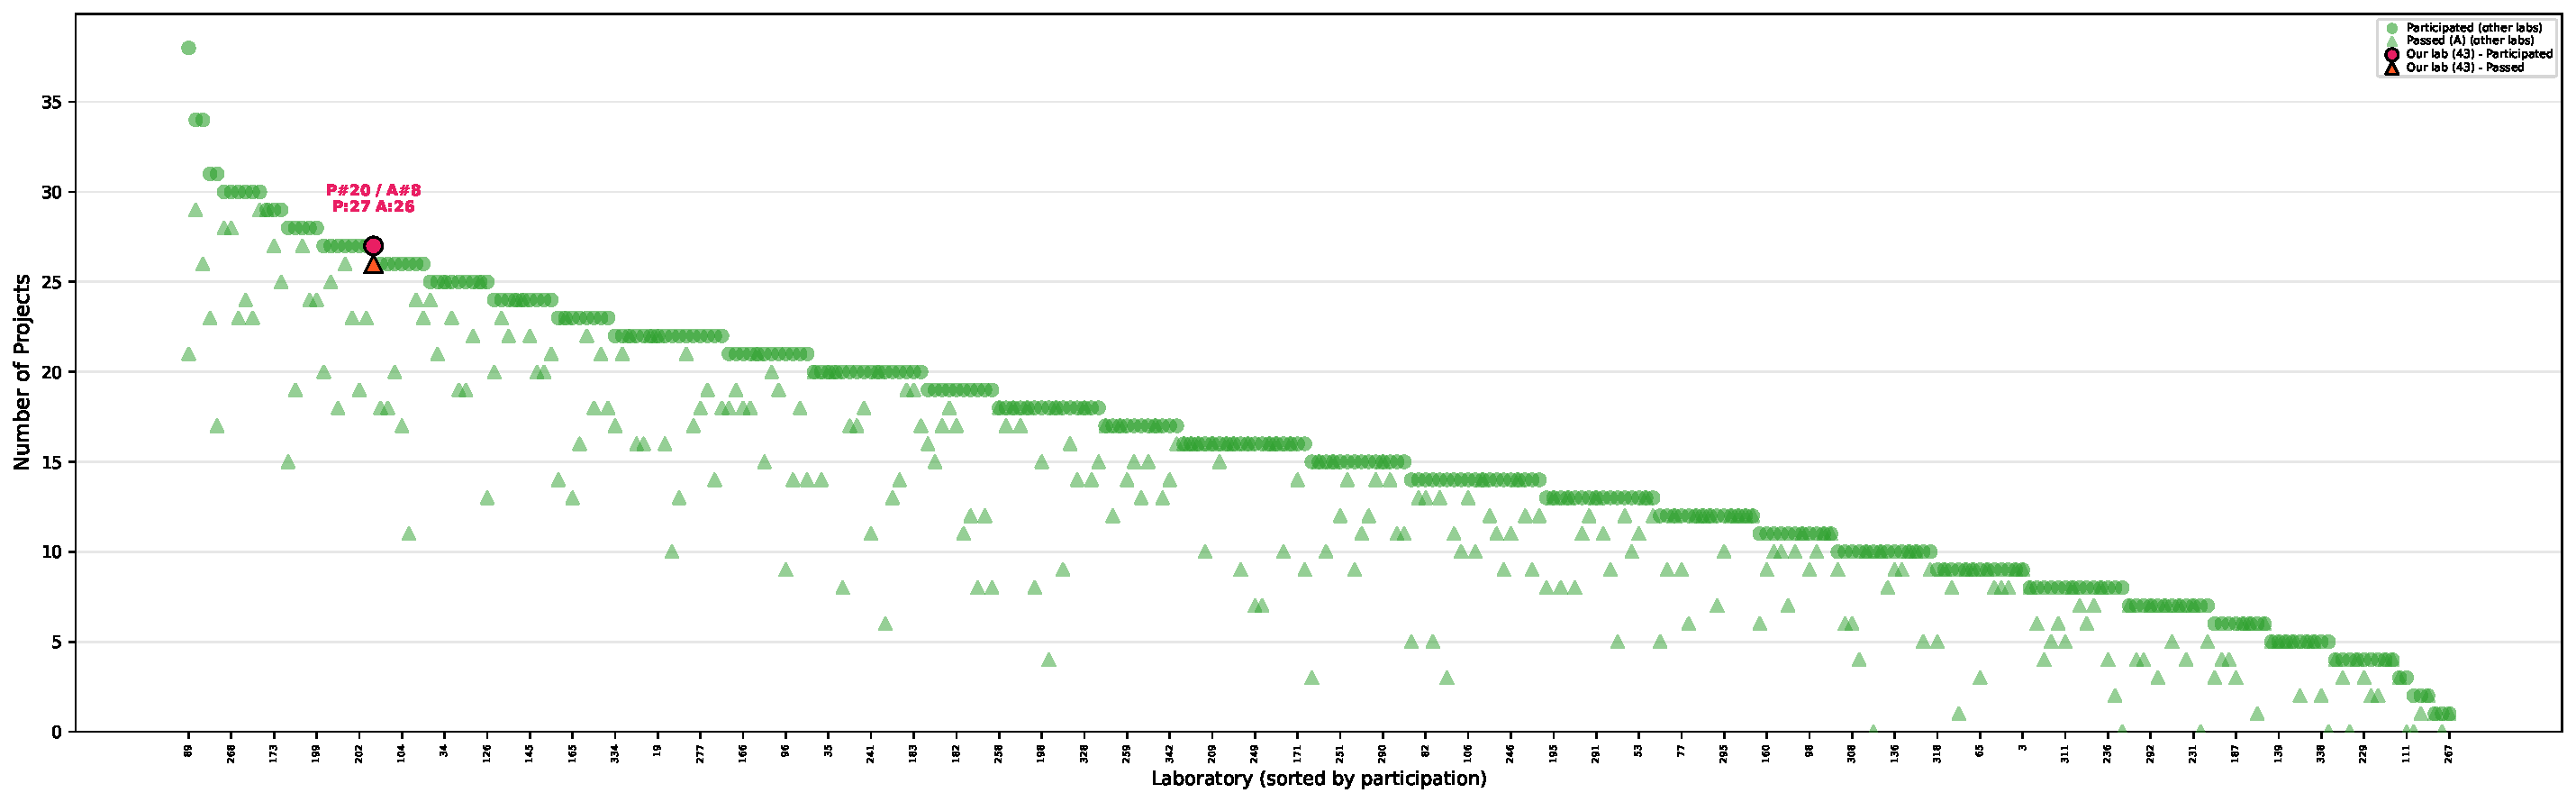
\includegraphics[width=\textwidth,height=4.5cm,keepaspectratio]{../paper/figures/fig_lab_performance_2023.pdf}\\[2pt]{\tiny 2023: P\#20/A\#8}
    \end{column}
  \end{columns}
  \vspace{0.1cm}
  \begin{columns}
    \begin{column}{0.33\textwidth}
      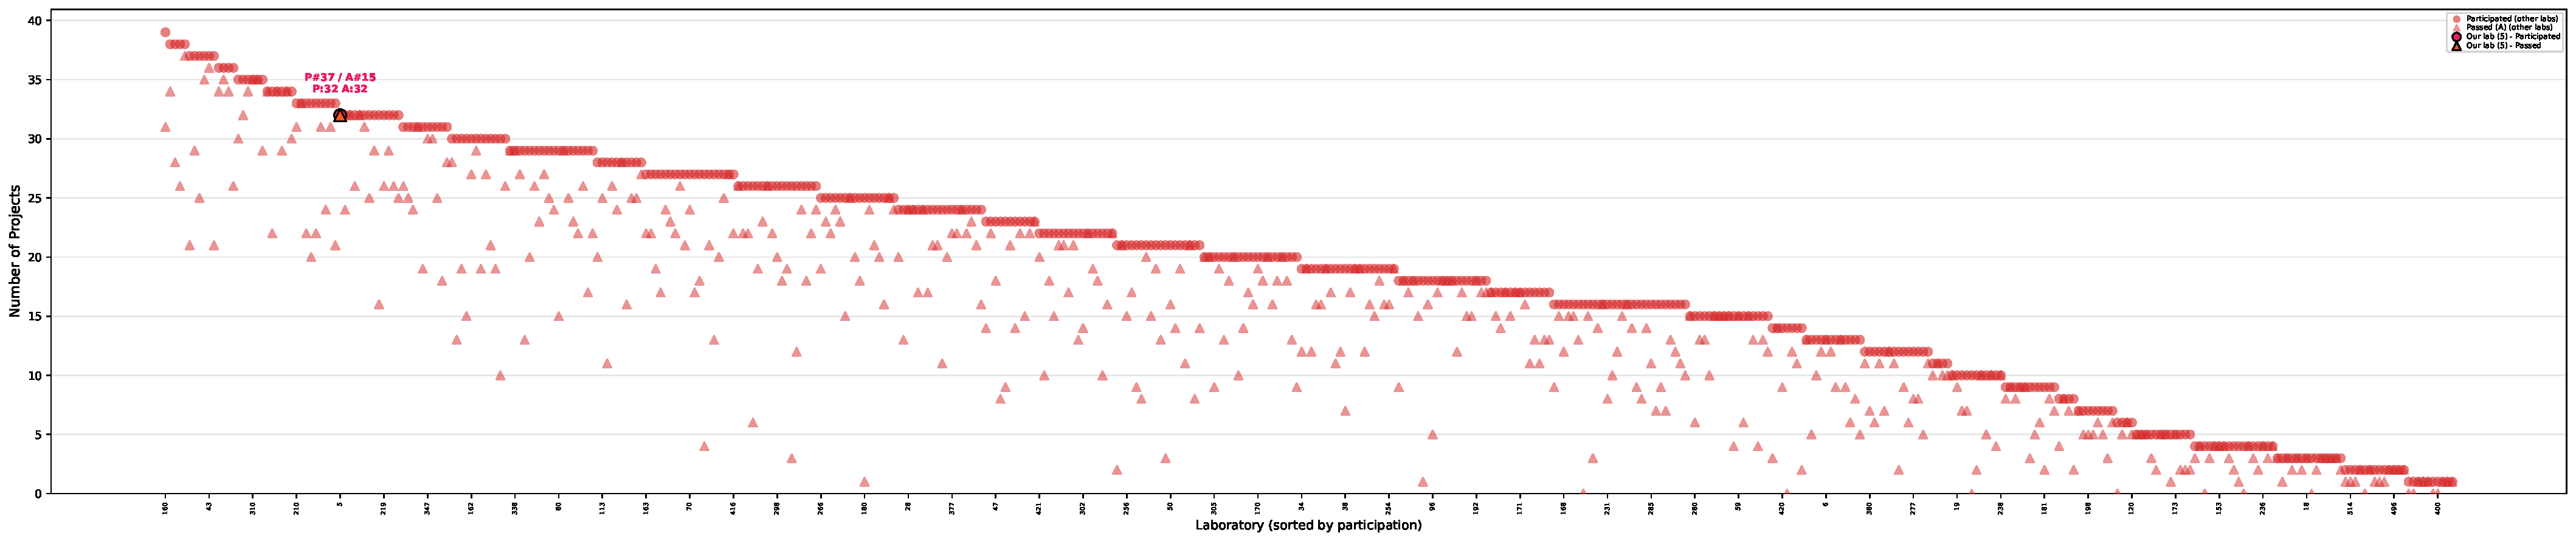
\includegraphics[width=\textwidth,height=4.5cm,keepaspectratio]{../paper/figures/fig_lab_performance_2024.pdf}\\[2pt]{\tiny 2024: P\#36/A\#15}
    \end{column}
    \begin{column}{0.33\textwidth}
      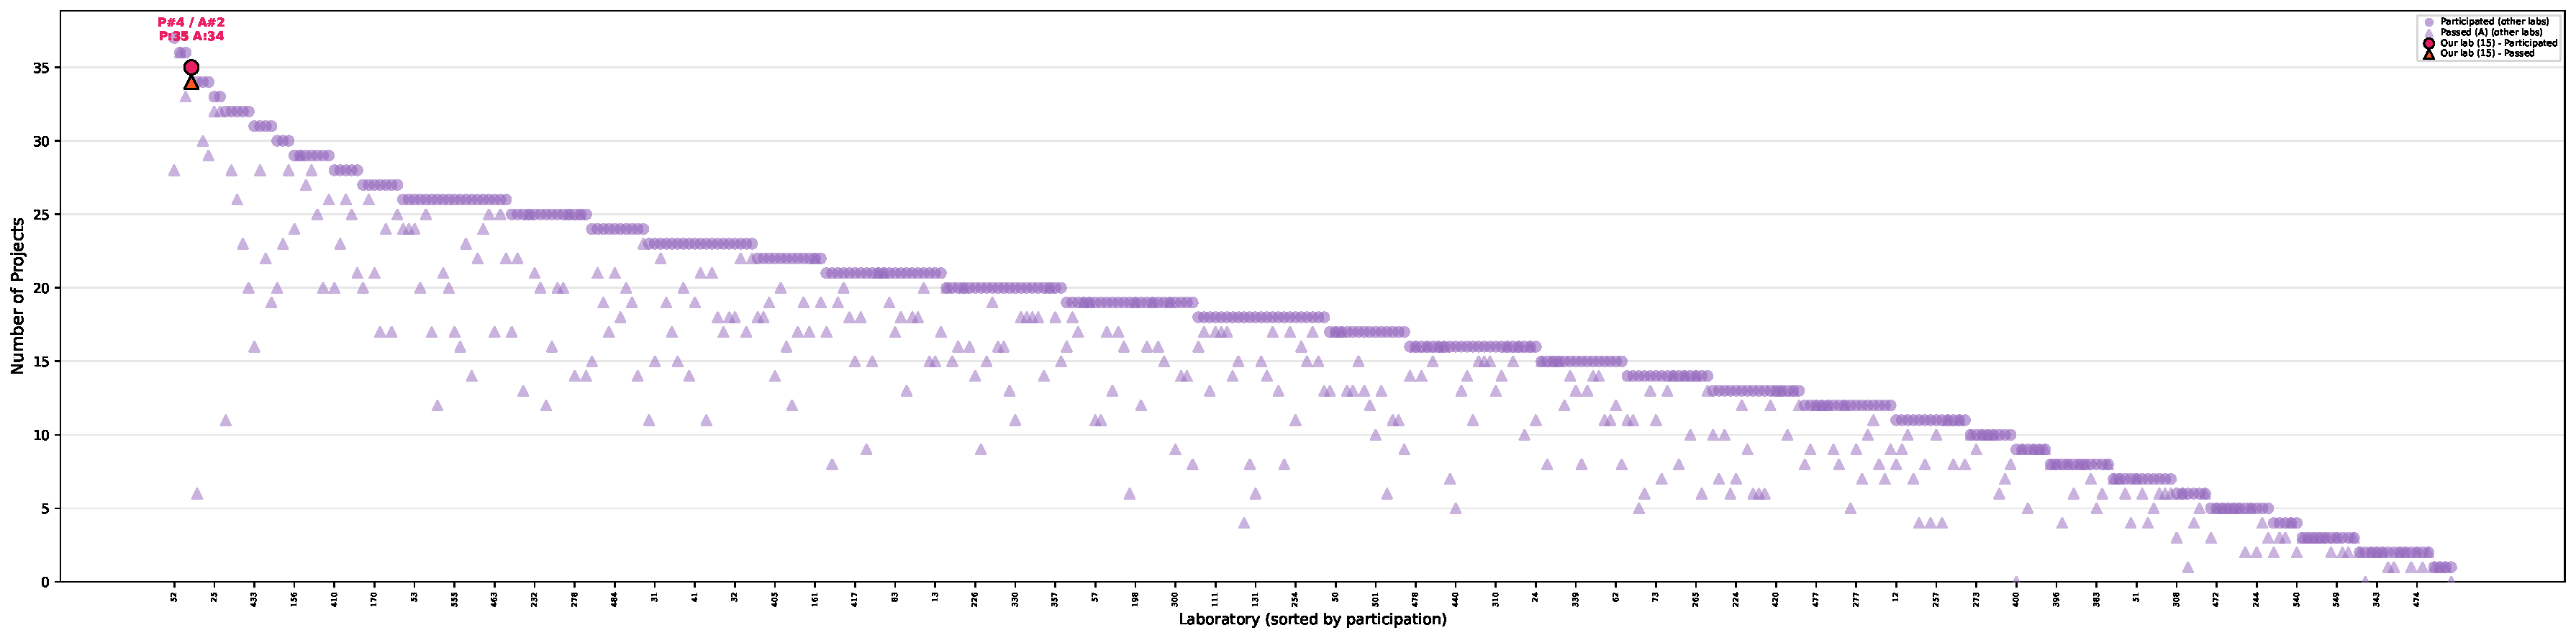
\includegraphics[width=\textwidth,height=4.5cm,keepaspectratio]{../paper/figures/fig_lab_performance_2025.pdf}\\[2pt]{\tiny 2025: P\#4/A\#2}
    \end{column}
    \begin{column}{0.33\textwidth}
      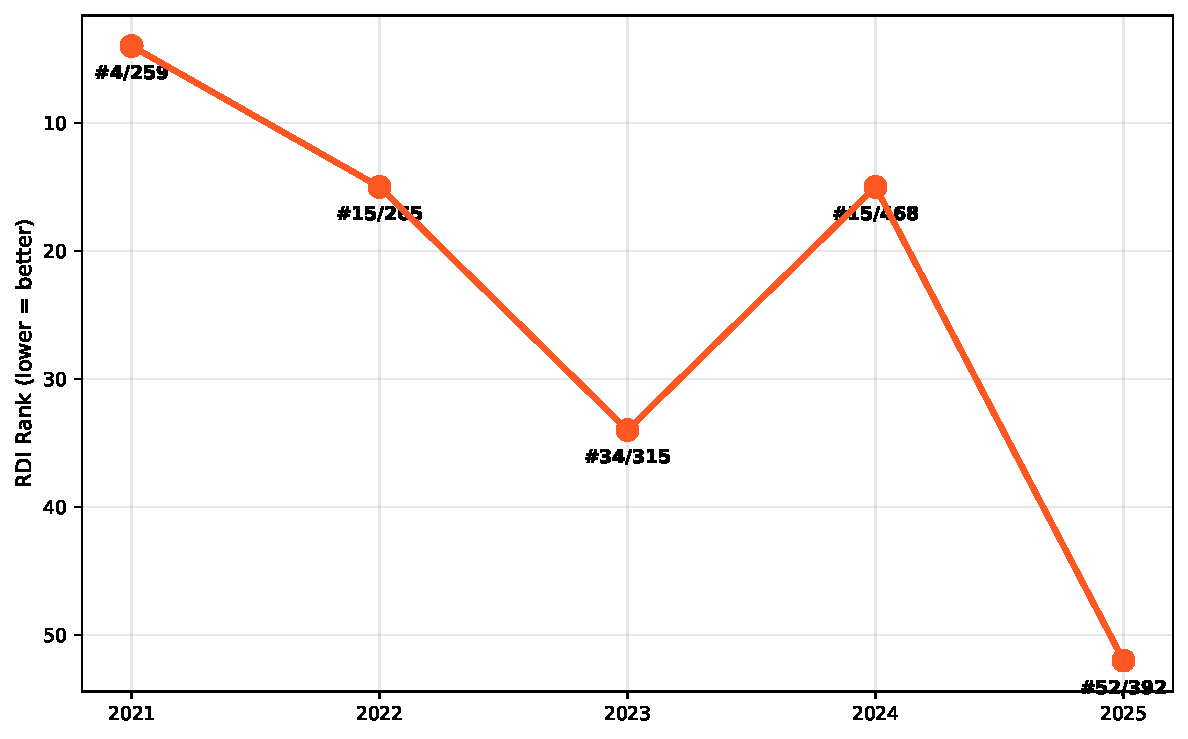
\includegraphics[width=\textwidth,height=4.5cm,keepaspectratio]{../paper/figures/fig_rdi_ranking.pdf}\\[2pt]{\tiny 加权RDI排名 (2021--2025)}
    \end{column}
  \end{columns}
\end{frame}
}

% --- Backup 6: RDI boxplot ---
{
\begin{frame}[plain]{备用：RDI 盒须图}
  \centering
  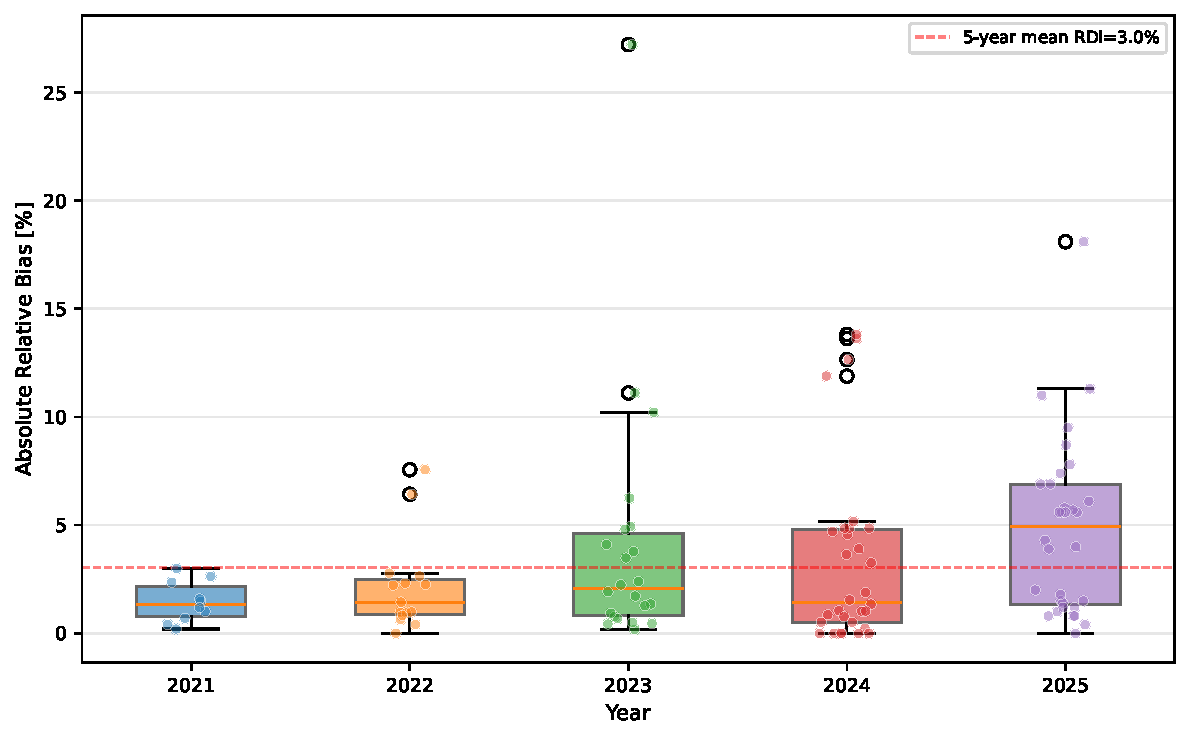
\includegraphics[width=0.55\textwidth,height=7cm,keepaspectratio]{../paper/figures/fig_rdi_boxplot.pdf}\\[4pt]
  {\small 本单位各年度 |相对偏差| 分布，虚线为5年加权均值 RDI (3.05\%)}
\end{frame}
}

\end{document}
